\ifdefined\ismainfile
\else
    \documentclass[11pt]{article}

    \makeatletter
\@ifclassloaded{revtex4-2}{}{\usepackage[margin=1in]{geometry}}
\makeatother
\usepackage{amsmath,amsthm,amsfonts,amssymb,mathrsfs}
\usepackage{graphicx}
\usepackage{cancel}
\usepackage{bm}
\usepackage{tikz}
\usepackage{csquotes}
\usepackage{tikz-3dplot}
\usepackage{physics}
\usepackage{dsfont}
\usepackage{float}
\usepackage{xcolor}
\usepackage{mathtools}
\usepackage{tcolorbox}
\makeatletter
\@ifclassloaded{revtex4-2}{\let\affil\affiliation
}{\usepackage{authblk}}
\makeatother

\tcbuselibrary{breakable}
\usepackage{keytheorems}
\newkeytheorem{definition}[parent=section, tcolorbox-no-titlebar={breakable, colback=blue!10}]
\newkeytheorem{example,lemma,conjecture,claim,theorem,proposition,corollary,fact,assumption,construction}[sibling=definition, tcolorbox-no-titlebar={breakable, colback=blue!10}]
\theoremstyle{definition}
\newtheorem{protocol}{Protocol}[section]

\newkeytheorem{remark}[parent=section, tcolorbox-no-titlebar={breakable}]
\allowdisplaybreaks[4]
\interdisplaylinepenalty=0
\makeatletter
\renewcommand{\log}{\mathop{\operator@font log}\nolimits}
\makeatother
\IfFileExists{bbm.sty}{\usepackage{bbm}}{\providecommand{\mathbbm}{\mathds}}
\usepackage{stmaryrd}
\usepackage{braket}
\makeatletter
\@ifpackageloaded{natbib}{}{\usepackage[numbers,sort&compress]{natbib}}
\makeatother
\usepackage{hyperref}
\usepackage[ruled,noline,longend]{algorithm2e}
\SetAlgoNoLine
\AtBeginDocument{\SetAlgoNoLine}
\SetAlgoLongEnd
\RestyleAlgo{boxruled}
\LinesNumbered
\definecolor{algcommentgray}{gray}{0.35}
\newcommand{\AlgCommentFont}[1]{\textcolor{algcommentgray}{#1}}
\SetCommentSty{AlgCommentFont}
\SetKwComment{tcp}{{\color{algcommentgray}$\blacktriangleright$}\ }{}
\usepackage{tcolorbox}
\tcbuselibrary{breakable}
\renewcommand{\topfraction}{0.9}
\renewcommand{\bottomfraction}{0.8}
\renewcommand{\textfraction}{0.07}
\renewcommand{\floatpagefraction}{0.85}
\setcounter{topnumber}{3}
\setcounter{totalnumber}{5}
\newenvironment{longalgorithm}[2][]{\begin{tcolorbox}[breakable, sharp corners, boxsep=0pt,
      boxrule=\algoheightrule, colframe=black, colback=white,
      left=18pt, right=4pt, top=5pt, bottom=5pt, #1]\refstepcounter{algocf}\noindent\hspace*{-14pt}{\textbf{\algorithmcfname~\thealgocf:} #2}\par
  \addcontentsline{loa}{algocf}{\protect\numberline{\thealgocf}#2}\par\nobreak\vspace{2pt}\nointerlineskip
  \moveleft18pt\vbox{\hrule width \dimexpr\linewidth+22pt\relax height \algoheightrule}\vspace{3pt}\setcounter{AlgoLine}{0}\RestyleAlgo{plain}}{\end{tcolorbox}}
\DontPrintSemicolon
\SetKwInput{KwIn}{Require}
\SetKwInput{KwOut}{Ensure}
\SetKwFor{For}{for}{do}{end for}
\SetKwFor{ForEach}{for each}{do}{end for}
\SetKwFor{While}{while}{do}{end while}
\makeatletter
\newenvironment{breakablealgorithm}{\par\addvspace{\intextsep}\hrule height .8pt\kern2pt
  \renewcommand{\caption}[2][]{\refstepcounter{algocf}\noindent\textbf{\algorithmcfname~\thealgocf:} ##2\par
    \kern2pt\hrule\kern2pt
    \ifx\relax##1\relax
      \addcontentsline{loa}{algocf}{\protect\numberline{\thealgocf}##2}\else
      \addcontentsline{loa}{algocf}{\protect\numberline{\thealgocf}##1}\fi
  }}{\par\kern2pt\hrule\addvspace{\intextsep}}
\makeatother
\usepackage{old-arrows}
\usepackage{color}
\usepackage{array, tabularx}
\usepackage{longtable}
\makeatletter
\@ifclassloaded{revtex4-2}{\appdef\@mkpream@relax{\let\@endpbox\relax}}{}
\makeatother
\usepackage{booktabs}
\newcolumntype{L}[1]{>{\raggedright\arraybackslash}p{#1}}
\newcolumntype{C}[1]{>{\centering\arraybackslash}p{#1}}
\newcolumntype{R}[1]{>{\raggedleft\arraybackslash}p{#1}}
\newcommand{\Circo}[0]{\mathfrak{C}}
\newcommand{\restrict}[2]{#1 \vert_{#2}}
\newcommand{\physq}[0]{\mathcal{M}}


\newcommand{\Xp}[0]{\mathcal{X}}
\newcommand{\Zp}[0]{\mathcal{Z}}

\newcommand{\nS}[1]{\mathbb{N}_{#1}}
\newcommand{\aS}[1]{\mathbb{C}_{#1}}

\newcommand{\nD}[1]{D^N_{#1}}
\newcommand{\aD}[1]{D^C_{#1}}

\newcommand{\control}[3]{C_{#1} {#2}_{#3}}
\usetikzlibrary{3d, shapes, arrows.meta, decorations.pathreplacing, decorations.markings, cd, shapes.geometric, calc}
\IfFileExists{tikzlibrarycalligraphy.code.tex}{\usetikzlibrary{calligraphy}}{}
\pgfkeysifdefined{/pgf/decoration/calligraphic brace/.@cmd}{}{\pgfkeys{/pgf/decoration/calligraphic brace/.style={brace}}}
\tikzstyle{midarrow} = [decoration={markings, mark= at position 0.6 with {\arrow{Stealth}}}, postaction={decorate}]
\renewcommand{\comment}[1]{{\color{red} #1}}

\newcommand{\YR}[1]{{\color{Teal} [Collin: #1]}}

\newcommand{\kc}[1]{{\color{cyan} [Katie: #1]}}

\newcommand{\bb}[1]{{\color{purple}[BB: #1]}}




\newcommand{\vva}[1]{{\color{magenta} [VVA: #1]}}









\newcommand{\al}[1]{{\color{DarkGreen} [Ana: #1]}}

\newcommand{\hp}[1]{{\color{brown} [Harry: #1]}}

\newcommand{\NT}[1]{{\color{orange} [NT: #1]}}

\newcommand{\dom}[1]{\textcolor{blue}{[Dom: #1]}}

\newcommand{\todo}[1]{\textcolor{blue}{[TO-DO: #1]}}

\newcommand{\new}[1]{{\color{DarkMagenta}#1}}
\definecolor{FGreen}{RGB}{58,158,92}
\definecolor{lightred}{RGB}{223, 123, 84}
\definecolor{lightbrown}{RGB}{242,216,199}
\definecolor{invisiblegray}{RGB}{238,238,237}
\definecolor{lightgreen}{RGB}{222, 235, 218}
\definecolor{lightcyan}{RGB}{153, 191, 216}
\definecolor{lightcyan2}{RGB}{208, 224, 235}
\definecolor{cyan2}{RGB}{144,201,226}
\definecolor{lightyellow}{RGB}{252, 238, 183}
\definecolor{OrangeRed}{RGB}{223,123,84}
\definecolor{CyanGreen}{RGB}{81,177,184}
\definecolor{rose}{RGB}{226,45,139}
\definecolor{Ycolor}{RGB}{248,236,104}
\definecolor{Hcolor}{RGB}{255,255,0}
\definecolor{Xcolor}{RGB}{246,143,138}
\definecolor{Zcolor}{RGB}{210,254,206}
\definecolor{Lred}{RGB}{244,163,163}
\definecolor{Lgreen}{RGB}{160,211,179}
\definecolor{Lblue}{RGB}{170,183,240}
\definecolor{tickcolor}{RGB}{181,0,250}
\definecolor{DarkBlue}{RGB}{14,38,80}
\definecolor{greenblue}{RGB}{0,255,127}
\definecolor{darkblue}{RGB}{57,85,134}
\definecolor{electrored}{RGB}{244,96,85}
\definecolor{electrored2}{RGB}{245,107,94}
\definecolor{BBXcheck}{RGB}{210,234,206}
\definecolor{BBZcheck}{RGB}{204,204,250}
\definecolor{softred}{RGB}{245,206,206}
\definecolor{fuchsiapurple}{RGB}{180, 0, 255}
\definecolor{Teal}{RGB}{62,138,141}
\definecolor{gold}{RGB}{233,168,58}
\definecolor{Crimson}{RGB}{220,20,60}
\definecolor{RedOrange}{RGB}{255,69,0}
\definecolor{DarkMagenta}{RGB}{139,0,139}
\definecolor{DarkGreen}{RGB}{0,100,0}
\definecolor{MidnightBlue}{RGB}{25,25,112}



\newcommand{\g}{\mathbf{g}}
\newcommand{\h}{\mathbf{h}}
\renewcommand{\k}{\mathbf{k}}
\newcommand{\f}{\mathbf{f}}
\newcommand{\C}{\mathbf{C}}
\newcommand{\Z}{\mathbb{Z}}
\renewcommand{\S}{\mathcal{S}}
\newcommand{\CC}{\mathcal{C}}
\newcommand{\charge}{k}
\newcommand{\totalcharge}{K}
\newcommand{\B}{\mathbb{B}}
\renewcommand{\O}{\mathcal{O}}
\newcommand{\Ocal}{\mathcal{O}}
\renewcommand{\Vec}{\mathcal{V}ec}
\newcommand{\Rep}{\text{Rep}}
\newcommand{\nnb}{\nonumber}
\newcommand{\lt}{\triangleleft}
\newcommand{\rt}{\triangleright}
\newcommand{\Lcal}{\mathcal{L}}
\newcommand{\Acal}{\mathcal{A}}
\newcommand{\Gcal}{\mathcal{G}}
\newcommand{\XX}{\mathcal{X}}
\newcommand{\YY}{\mathcal{Y}}
\newcommand{\ZZ}{\mathcal{Z}}
\newcommand{\Com}[2]{[ #1, #2 ]}
\newcommand{\ComGrp}[2]{[ #1, #2 ]_{\text{grp}}}
\newcommand{\level}{\operatorname{Lv}}
\newcommand{\code}{\mathcal{C}}


\newcommand{\glosym}[0]{\mathsf{L}}
\newcommand{\im}{\operatorname{im}}
\newcommand{\rk}{\operatorname{rk}}
\newcommand{\supp}[1]{\operatorname{Supp}(#1)}
\newcommand{\Ad}{\operatorname{Ad}}
\newcommand{\Irrep}{\operatorname{Irrep}}
\newcommand{\Wt}{\operatorname{Wt}}
\newcommand{\Lin}{\mathfrak{L}}
\newcommand{\interior}{\operatorname{int}}
\newcommand{\T}[0]{\mathsf{U}}
\newcommand{\orbit}[1]{O^{\mathcal{T}}(#1)}
\newcommand{\sym}[0]{\overline{S}}
\newcommand{\av}[0]{\mathbb{A}_v}
\newcommand{\bp}[0]{\mathbb{B}_f}
\newcommand{\onsite}[1]{\mathsf{T}|_{#1}}
\newcommand{\Log}[1]{\overline{#1}}
\newcommand{\id}[0]{\mathbf{1}}
\newcommand{\bd}[1]{\delta({#1})}
\newcommand{\zp}[0]{\mathbb{Z}_p}
\newcommand{\cX}[0]{\mathcal{X}}
\newcommand{\cZ}[0]{\mathcal{Z}}
\newcommand{\cC}[0]{\mathcal{C}}
\newcommand{\cE}[0]{\mathcal{E}}
\newcommand{\cx}[2]{CX_{#1\rightarrow#2}}
\newcommand{\wcp}[2]{\mathcal{C}P_{#1\rightarrow#2}}
\newcommand{\wcx}[2]{\mathcal{C}X_{#1\rightarrow#2}}
\newcommand{\wcz}[2]{\mathcal{C}Z_{#1\rightarrow#2}}
\newcommand{\wcy}[2]{\mathcal{C}Y_{#1\rightarrow#2}}
\newcommand{\cpw}[2]{C\mathcal{P}_{#1\rightarrow#2}}
\newcommand{\cxw}[2]{C\mathcal{X}_{#1\rightarrow#2}}
\newcommand{\czw}[2]{C\mathcal{Z}_{#1\rightarrow#2}}
\newcommand{\cyw}[2]{C\mathcal{Y}_{#1\rightarrow#2}}
\newcommand{\wct}[2]{\mathcal{C}\mathcal{T}_{#1\rightarrow#2}}
\newcommand{\wctdag}[2]{\mathcal{C}\mathcal{T}^\dagger_{#1\rightarrow#2}}
\newcommand{\cnot}[0]{\CNOT}
\newcommand{\SWAP}[0]{\mathsf{SWAP}}
\newcommand{\CNOT}[0]{\mathsf{CNOT}}
\newcommand{\CSWAP}[0]{\mathsf{CSWAP}}
\newcommand{\CX}[0]{\mathsf{CX}}
\newcommand{\CZ}[0]{\mathsf{CZ}}
\newcommand{\CT}[0]{\mathsf{CU}}
\newcommand{\swap}[0]{\SWAP}
\newcommand{\cswap}[0]{\CSWAP}

\newcommand{\overlap}[1]{\Omega(#1)}
\newcommand{\E}[2]{e_{(#1,#2)}}
\newcommand{\dec}[1]{\tilde{#1}}
\newcommand{\insuppof}[2]{#1|_{#2}}
\newcommand{\plushalf}[1]{{#1+\frac{1}{2}}}
\newcommand{\minushalf}[1]{{#1-\frac{1}{2}}}
\newcommand{\scrG}[0]{{\mathscr{G}}}
\newcommand{\sset}[1]{\Sigma(#1)}

\newcommand{\symOP}{\T}
\newcommand{\symS}{\overline{S}}
\newcommand{\haH}{\mathsf{H}}
\newcommand{\haA}{\mathsf{A}}
\newcommand{\haB}{\mathsf{B}}
\newcommand{\haP}{\mathsf{P}}
\newcommand{\haQ}{\mathsf{Q}}
\newcommand{\haX}{\mathsf{X}}
\newcommand{\Deco}{\mathfrak{D}}

\newcommand{\vertexset}[1]{\Sigma^{-1}(#1)}
\newcommand{\invvertexset}[1]{\Sigma(#1)}
\newcommand{\faceP}{\mathcal{P}} 
\newcommand{\vertexV}{\mathsf{V}}
\newcommand{\edgeE}{\mathsf{E}}
\newcommand{\faceF}{\mathsf{F}}
\newcommand{\graphG}{\mathsf{G}}
\newcommand{\intG}{\mathbb{G}}
\newcommand{\N}{\mathsf{N}}
\newcommand{\eigenE}{\mathbf{E}} 
\newcommand{\gaugedA}{\mathbb{A}}
\newcommand{\gaugedB}{\mathbb{B}}
\newcommand{\gaugedS}{\mathbb{S}}
\newcommand{\Sdec}{\mathfrak{s}}
\providecommand{\vr}{}
\renewcommand{\vr}{v_r}
\newcommand{\gaugedH}{\mathbb{H}}
\newcommand{\gaugingOP}{\mathscr{G}}
\newcommand{\chproj}[2]{\llbracket #1\rrbracket _{#2}}

\newcommand{\gX}{\mathcal{X}}
\newcommand{\gZ}{\mathcal{Z}}
\newcommand{\mX}{\mathcal{X}}
\newcommand{\mZ}{\mathcal{Z}}
\newcommand{\gW}{\mathcal{W}}
\newcommand{\gY}{\mathcal{Y}}
\newcommand{\Agrp}{\mathbf{A}}
\newcommand{\chOmega}{\mathit{\Omega}}
\newcommand{\Linex}{\Lin_{\rm ex}(\mathcal H_{\rm m})}
\newcommand{\Linnt}{\Lin_{\rm nt}^{\rm ex}(\mathcal H_{\rm mat})}


\newcommand{\K}{\mathcal{K}}
\newcommand{\gaugedT}{\mathbb{T}}
\newcommand{\Stab}{\mathcal{G}}
\newcommand{\F}{\mathcal{F}}
\newcommand{\Hp}{\mathcal{H}}
\newcommand{\Poly}{\mathsf{Poly}}
\newcommand{\Fphys}{F_{\text{phys}}}
\newcommand{\Fmeas}{F_{\text{meas}}}
\newcommand{\Fp}{\mathbf{F}_p}
\newcommand{\Zq}{\mathbb{Z}_q}
\newcommand{\Sprod}[2]{\Lambda\left( #1, #2 \right)}
\newcommand{\FT}{F^T}
\newcommand{\nbhd}{\mathsf{N}}

\newcommand{\Cgeom}{C_{\text{geom}}}
\newcommand{\CLDPC}{C_{\text{LDPC}}}
\newcommand{\Cstep}{C_{\text{step}}}
\newcommand{\Cretract}{C_{\text{retract}}}
\newcommand{\Ctotal}{C_{\text{total}}}
\newcommand{\Cgauge}{C_{\text{gauge}}}

\newcommand{\nonabel}[1]{S^\mathrm{N}_{#1}}
\newcommand{\abel}[1]{S^\mathrm{A}_{#1}}
\newcommand{\gnonabel}[1]{\mathbb{S}^\mathrm{N}_{#1}}
\newcommand{\gabel}[1]{\mathbb{S}^\mathrm{A}_{#1}}
\newcommand{\onset}[2]{{#1}_{\sset{#2}}}
\newcommand{\ccomm}[2]{[#1,#2]_{\mathrm{grp}}}
\newcommand{\tu}[0]{t_{\mathrm{u}}}
\newcommand{\tg}[0]{t_{\mathrm{g}}}
\newcommand{\tf}[0]{t_\mathrm{f}}
\newcommand{\Ig}[0]{\mathrm{I}_{\mathrm{g}}}
\newcommand{\Ifn}[0]{\mathrm{I}_\mathrm{f}}
\newcommand{\Ib}[0]{\mathrm{I}_0}
\newcommand{\cA}[0]{\mathcal{A}}
\newcommand{\cQ}[0]{\mathcal{Q}}
\newcommand{\cK}[0]{\mathcal{K}}
\newcommand{\grpcom}[2]{\ComGrp{#1}{#2}}
\newcommand{\de}[0]{d_\mathcal{E}}



\definecolor{Teal}{RGB}{0,128,128}
\definecolor{Crimson}{RGB}{220,20,60}
\definecolor{RedOrange}{RGB}{255,69,0}
\definecolor{DarkMagenta}{RGB}{139,0,139}
\definecolor{DarkGreen}{RGB}{0,100,0}
\definecolor{MidnightBlue}{RGB}{25,25,112}


\hypersetup{
    colorlinks=true,
    linkcolor=MidnightBlue,
    citecolor=MidnightBlue,
    urlcolor=MidnightBlue,}

\usepackage{amsfonts,latexsym,amsthm,amssymb,amsmath,amscd,euscript,tikz,mathtools}
\usepackage{framed}
\usepackage[normalem]{ulem}
\makeatletter
\@ifclassloaded{revtex4-2}{}{\usepackage[margin=1in]{geometry}}
\makeatother
\usepackage{color}




\usepackage{enumitem}
\usepackage{environ}
\usepackage{dcolumn}

\usetikzlibrary{positioning, shadows, arrows, backgrounds, fit}
\usetikzlibrary{decorations.pathmorphing}

\definecolor{Teal}{RGB}{0,128,128}

\hypersetup{
    colorlinks=true,
    linkcolor=MidnightBlue,
    citecolor=MidnightBlue,
    urlcolor=MidnightBlue,
}

\definecolor{GrayOut}{gray}{0.8}
\NewEnviron{GrayedOut}{\begingroup\color{GrayOut}\BODY\endgroup
}

\newcommand{\diam}{\operatorname{diam}}
\newcommand{\dist}{\operatorname{dist}}

\newcommand{\cH}{\mathcal{H}}
\newcommand{\cT}{\mathcal{T}}
\newcommand{\cN}{\mathcal{N}}
\newcommand{\cB}{\mathcal{B}}
\newcommand{\bbP}{\mathbb{P}}
\newcommand{\haT}{\mathsf{T}}
\newcommand{\haD}{\mathsf{D}}
\newcommand{\cF}{\mathcal{F}}

\newcommand{\CZero}{C_0(\Gcal_0)}
\newcommand{\COne}{C_1(\Gcal_1)}
\newcommand{\deltaOne}{\delta_1}
\newcommand{\jall}{\mathbf{1}}
\newcommand{\tof}[0]{\ket{\mathsf{Tof}}}
\newcommand{\Pp}[1]{\mathrm{P}^+_{\Log{#1}}}
\newcommand{\Ppk}[1]{\mathrm{P}^+_{\Log{#1}^{\otimes k}}}
\newcommand{\Pm}[1]{\mathrm{P}^-_{\Log{#1}}}

\newcommand{\fa}[0]{F_\mathrm{A}}
\newcommand{\fn}[0]{F_\mathrm{N}}

\newcommand{\CHANGE}[1]{{\color{DarkMagenta}#1}}

\newcommand{\syndromeSet}{\sigma}
\newtheorem{axiom}{Axiom}[section]
\newtheorem{question}{Question}[section]


\newcommand{\green}[1]{\textcolor{Teal}{#1}}
\newcommand{\blue}[1]{\textcolor{blue}{#1}}
\newcommand{\red}[1]{\textcolor{red}{#1}}

\makeatletter
\let\UncappedLeft\left
\let\UncappedRight\right
\def\left{\@ifnextchar({\CappedLeftParen}{\UncappedLeft}}
\def\CappedLeftParen(#1\right{\@ifnextchar){\CappedRightParen{#1}}{\UncappedLeft(#1\UncappedRight}}
\def\CappedRightParen#1){\mathopen{}\bigg(#1\bigg)\mathclose{}}
\makeatother

\definecolor{vred}{rgb}{0.85,0,0}
\definecolor{epur}{cmyk}{0.45,0.86,0,0}
\definecolor{poraBase}{cmyk}{0,0.42,1,0}
\colorlet{pora}{poraBase!90!black}
\definecolor{setgray}{RGB}{225,225,225}
\newcommand{\vC}[1]{{\color{vred}#1}}
\newcommand{\eC}[1]{{\color{epur}#1}}
\newcommand{\pC}[1]{{\color{pora}#1}}
\newcommand{\sq}[9]{\left(\begin{smallmatrix}
\vC{#1} & \eC{#2} & \vC{#3}\\[1pt]
\eC{#4} & #5 & \eC{#6}\\[1pt]
\vC{#7} & \eC{#8} & \vC{#9}
\end{smallmatrix}\right)}
\newcommand{\mm}[4]{\begin{smallmatrix}#1 & #2\\ #3 & #4\end{smallmatrix}}
\newcommand{\sqe}[5]{\sq{\cdot}{#1}{\cdot}{#2}{#3}{#4}{\cdot}{#5}{\cdot}}
\newcommand{\Sg}{\mathsf{S}}
\newcommand{\CZbar}{\overline{CZ}}

\setcounter{tocdepth}{1}

    
    \begin{document}
    \title{Examples}
    \date{\today}
    \bibliographystyle{abbrv}

    \maketitle
\fi


In this section we present a range of examples that demonstrate the flexibility of the general Clifford gauging measurement protocol. These examples include local topological codes as well as more general QLDPC codes that are not local in any fixed spatial dimension. We focus our discussion on finding the deformed gauged codes that occur during the gauging measurement protocol in each example. The logical action of the gauging measurement protocol in each case is simply to measure the relevant transversal Clifford gate on the initial stabilizer code. We discuss applications of such logical measurements in the following section, below. 

\subsection{Gauging XS on the color code}
We start with Clifford gauging on the color code as a pedagogical example, before moving to higher-rate examples. First, as the color code is self-dual, it possesses a transversal $XS$ gate. If we gauge this symmetry, we can obtain $\ket{\CZbar}$ states on the color code. 

We begin by partitioning the sites of the honeycomb lattice into vertex sets. There are many choices of such a partition, with three convenient ones being (i) one site per vertex set, (ii) one unit cell (two sites) per vertex set, and (iii) disjoint hexagons forming vertex sets. For this example, we will consider all three choices to give a sense for how the resulting models differ. We note that a similar protocol to $(i)$ was considered in~\cite{Tantivasadakarn23}. 

The precise form of the $XS$ symmetry on the honeycomb lattice is \begin{equation}
    \T = \prod_{A} W \prod_B \tilde{W}, \quad W = T^\dagger X T = e^{-i\pi/4}XS, \quad \tilde{W} = TXT^\dagger = e^{+i\pi/4}XS^\dagger
\end{equation} As the honeycomb lattice is bipartite, it can be separated into two sublattices $A, B$. Going forward, we will denote $A$ sites with black circles and $B$ sites with white circles.

We use the following commutation relations when performing the gauging procedure: 
\begin{equation}
    \begin{aligned}
    CW_{c \rightarrow t} X_c [CW_{c \rightarrow t}]^\dagger &= X_c \otimes W_t \\
    C\tilde{W}_{c \rightarrow t} X_c [C\tilde{W}_{c \rightarrow t}]^\dagger &= X_c \otimes \tilde{W}_t \\
    CW_{c \rightarrow t} X_t [CW_{c \rightarrow t}]^\dagger &= X_t S_c^\dagger \CZ_{c \to t} \\
    C\tilde{W}_{c \rightarrow t} X_t [C\tilde{W}_{c \rightarrow t}]^\dagger &= X_t S_c \CZ_{c \to t} \\
    \end{aligned}
\end{equation}
\begin{equation}
\begin{aligned}
    CW_{c \rightarrow t} Z_t [CW_{c \rightarrow t}]^\dagger =
    C\tilde{W}_{c \rightarrow t} Z_t [C\tilde{W}_{c \rightarrow t}]^\dagger = Z_c \otimes Z_t
\end{aligned}
\end{equation}


\subsubsection{Qubit Per Vertex Set}
As our first example, we take vertex sets to be single sites of the honeycomb lattice. We introduce a new ancilla qubit for every vertex set, initialized in the $\ket{+}$ state, and we entangle it with its vertex set by applying a $CW$ or $C\tilde{W}$ gate depending on the sublattice. The ancilla acts as the control, and the code qubit as the target.

The new stabilizers after this step are as follows: 
\begin{equation}
    \raisebox{-35pt}{
    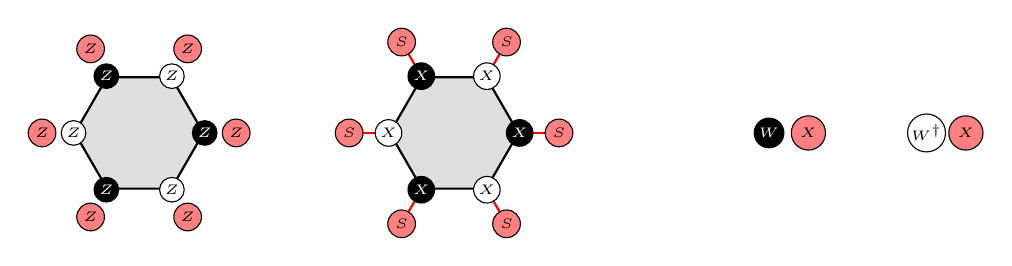
\begin{tikzpicture}

        \node[name=g, regular polygon, regular polygon sides = 6, draw, inner sep = 0.5cm, fill=gray, fill opacity=0.25, thick] at (-4, 0) {};
        
        \foreach \anchor/\placement/\n/\fill/\text in
        {corner 1/below/1/white/black, corner 2/below/2/black/white, corner 3/right/3/white/black, corner 4/above/4/black/white, corner 5/above/5/white/black, corner 6/left/6/black/white}
        {
        \filldraw[shift=(g.\anchor), fill=red!50!white] (\n*60:0.4) circle (5pt);
        \node[inner sep = 1pt] at ($(g.\anchor) + (\n*60:0.4)$) {\tiny{$Z$}};
        \node[draw, circle, fill=\fill, inner sep = 1pt, text=\text] at (g.\anchor) {\tiny{$Z$}};
        }

        \node[name=g, regular polygon, regular polygon sides = 6, draw, inner sep = 0.5cm, fill=gray, fill opacity=0.25, thick] at (0, 0) {};
        
        \foreach \anchor/\placement/\n/\fill/\text in
        {corner 1/below/1/white/black, corner 2/below/2/black/white, corner 3/right/3/white/black, corner 4/above/4/black/white, corner 5/above/5/white/black, corner 6/left/6/black/white}
        {
        \draw[-, red, thick] ($(g.\anchor) + (\n*60:0.5)$) to (g.\anchor);
        \filldraw[shift=(g.\anchor), fill=red!50!white] (\n*60:0.5) circle (5pt);
        \node[draw, circle, fill=\fill, inner sep = 1pt, text=\text] at (g.\anchor) {\tiny{$X$}};
        }

        \foreach \n/\anchor in
        {1/corner 1,3/corner 3,5/corner 5}
        {
        \node[inner sep = 1pt] at ($(g.\anchor) + (\n*60:0.5)$) {\tiny{$S$}};
        }
        \foreach \n/\anchor in
        {2/corner 2,4/corner 4,6/corner 6}
        {
        \node[inner sep = 1pt] at ($(g.\anchor) + (\n*60:0.5)$) {\tiny{$S$}};
        }
        
        \node[draw, circle, fill=black, inner sep = 1pt, text=white] at (4, 0) {\tiny{$W$}};
        \node[draw, circle, fill=red!50!white, inner sep = 2pt] at (4.5, 0) {\tiny{$X$}};

        \node[draw, circle, fill=white, inner sep = 0.5pt, text=black] at (6, 0) {\tiny{$W^\dagger$}};
        \node[draw, circle, fill=red!50!white, inner sep = 2pt] at (6.5, 0) {\tiny{$X$}};
        
    \end{tikzpicture}
    }\label{eq:honeycomb_X_term_with_ancilla_vertices}
\end{equation}
Here we have displaced the red circles to avoid overlap for visual clarity; the red nodes also sit on vertices of the honeycomb lattice. A $\CZ$ gate is denoted by a red line between both degrees of freedom acted on by the gate.

We now introduce edges between the vertex set ancillas using the following rule: there must be a path connecting two ancillas if there exists a stabilizer with support on both the vertex sets associated with the ancillas. Since every vertex set is a single site, one way to satisfy this rule is to simply place the ancillas on the sites of another honeycomb lattice, sitting on top of the original one. The purple node and the red node correspond to the ancilla qubits on the edges and the vertices of the gauging graph, respectively.
We then add a new qubit on each edge of this new lattice (called the gauging graph). The new qubits are initialized in the $\ket{0}$ state. We entangle the new ancillas and the original vertex set ancillas using a cluster state entangler. The new stabilizers are as follows:
\begin{equation}
\raisebox{-30pt}{
    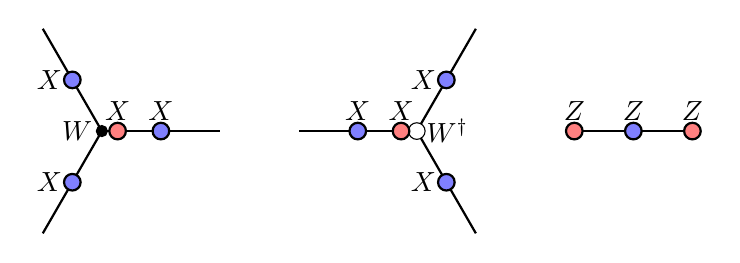
\begin{tikzpicture}
        \filldraw[] (0,0) circle (2pt) node[left] {$W$};
        \draw[-, thick] (0, 0) -- (1.5, 0);
        \draw[-, thick] (0, 0) -- (120:1.5);
        \draw[-, thick] (0, 0) -- (240:1.5);

        \filldraw[fill=blue!50!white, thick] (0:0.75) circle (3pt) node[above] {$X$};
        \filldraw[fill=blue!50!white, thick] (120:0.75) circle (3pt) node[left] {$X$};
        \filldraw[fill=blue!50!white, thick] (240:0.75) circle (3pt) node[left] {$X$};
        
        \filldraw[fill=red!50!white, thick] (0.2,0) circle (3pt) node[above] {$X$};

        
        \draw[-, thick] (4, 0) -- (2.5, 0);
        \draw[-, thick] (4, 0) -- ($(4, 0) + (60:1.5)$);
        \draw[-, thick] (4, 0) -- ($(4, 0) + (300:1.5)$);
        \filldraw[fill=white] (4,0) circle (3pt) node[right] {$W^\dagger$};

        \filldraw[fill=blue!50!white, thick] ($(4, 0) + (180:0.75)$) circle (3pt) node[above] {$X$};
        \filldraw[fill=blue!50!white, thick] ($(4, 0) + (60:0.75)$) circle (3pt) node[left] {$X$};
        \filldraw[fill=blue!50!white, thick] ($(4, 0) + (300:0.75)$) circle (3pt) node[left] {$X$};
        
        \filldraw[fill=red!50!white, thick] (3.8, 0) circle (3pt) node[above] {$X$};

        
        \draw[-, thick] (0+6, 0) -- (1.5+6, 0);
        \filldraw[fill=red!50!white, thick] (0+6,0) circle (3pt) node[above] {$Z$};
        \filldraw[fill=red!50!white, thick] (1.5+6, 0) circle (3pt) node[above] {$Z$};
        \filldraw[fill=blue!50!white, thick] (0.75+6, 0) circle (3pt) node[above] {$Z$};

    \end{tikzpicture}
    }
\end{equation} Note that the hexagonal stabilizers originating from the color code itself are unchanged by this step.

Finally, we project the vertex set ancillas onto the $\ket{+}$ state (in a real protocol, we would measure in the $X$ basis and then apply feedback to correct undesired $-1$ outcomes). The surviving stabilizers are those that commute with $X$ on the ancilla. Some are straightforward to determine--- the vertex stabilizers clearly commute with $X$, as they have only $X$ support on the vertex ancilla. Additionally, the product of the vertex-edge-vertex ancilla stabilizers $Z_{v} Z_{e} Z_{v'}$ around any hexagon will have no support on the vertex ancilla, and so trivially commutes.  
\begin{equation}
    \raisebox{-30pt}{
    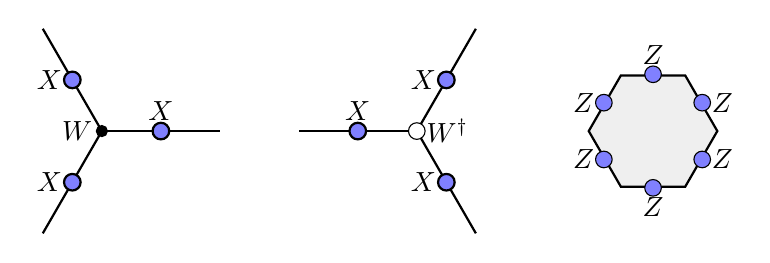
\begin{tikzpicture}
        \filldraw[] (0,0) circle (2pt) node[left] {$W$};
        \draw[-, thick] (0, 0) -- (1.5, 0);
        \draw[-, thick] (0, 0) -- (120:1.5);
        \draw[-, thick] (0, 0) -- (240:1.5);

        \filldraw[fill=blue!50!white, thick] (0:0.75) circle (3pt) node[above] {$X$};
        \filldraw[fill=blue!50!white, thick] (120:0.75) circle (3pt) node[left] {$X$};
        \filldraw[fill=blue!50!white, thick] (240:0.75) circle (3pt) node[left] {$X$};

        
        \draw[-, thick] (4, 0) -- (2.5, 0);
        \draw[-, thick] (4, 0) -- ($(4, 0) + (60:1.5)$);
        \draw[-, thick] (4, 0) -- ($(4, 0) + (300:1.5)$);
        \filldraw[fill=white] (4,0) circle (3pt) node[right] {$W^\dagger$};

        \filldraw[fill=blue!50!white, thick] ($(4, 0) + (180:0.75)$) circle (3pt) node[above] {$X$};
        \filldraw[fill=blue!50!white, thick] ($(4, 0) + (60:0.75)$) circle (3pt) node[left] {$X$};
        \filldraw[fill=blue!50!white, thick] ($(4, 0) + (300:0.75)$) circle (3pt) node[left] {$X$};


        \node[name = h, regular polygon, regular polygon sides = 6, draw, inner sep = 0.5cm, fill=gray!50!white, fill opacity=0.25, thick] at (7, 0) {};
        \foreach \anchor/\placement in
        {side 1/above, side 2/left, side 3/left, side 4/below, side 5/right, side 6/right}
        {
        \filldraw[shift=(h.\anchor), fill=blue!50!white] (0,0) circle (3pt) node[\placement] {$Z$};
        }
    \end{tikzpicture}
    }
\end{equation} These are the $A_v$ and $B_p$ terms, to use the notation of the previous sections.

Now we consider the original hexagon stabilizers of the color code, which have been deformed by the gauging procedure so far. The $Z$ hexagon does not commute with the measurement due to the $Z$ support it picked up on the vertex qubits; we can get rid of this support by multiplying with the three-body cluster state stabilizer $Z_v Z_e Z_{v'}$.
\begin{equation}
    \raisebox{-35pt}{
    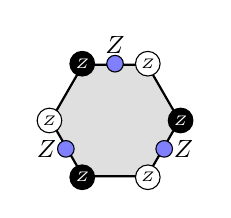
\begin{tikzpicture}

        \node[name=g, regular polygon, regular polygon sides = 6, draw, inner sep = 0.5cm, fill=gray, fill opacity=0.25, thick] at (-4, 0) {};
        
        \foreach \anchor/\placement/\n/\fill/\text in
        {corner 1/below/1/white/black, corner 2/below/2/black/white, corner 3/right/3/white/black, corner 4/above/4/black/white, corner 5/above/5/white/black, corner 6/left/6/black/white}
        {
        \node[draw, circle, fill=\fill, inner sep = 1pt, text=\text] at (g.\anchor) {\tiny{$Z$}};
        }

        \foreach \anchor/\placement in {side 1/above, side 3/left, side 5/right}
        \filldraw[shift=(g.\anchor), fill=blue!50!white] (0,0) circle (3pt) node[\placement] {\small{$Z$}};
        
    \end{tikzpicture}
    }
\end{equation} The $X$ hexagon is a little trickier--- we will again use the three-body cluster state stabilizer. We will use the following identity:
\begin{equation}
\begin{aligned}
    \CZ_{a \rightarrow b} &= \ket{0}\bra{0}_a \otimes \mathbb{I}_b + \ket{1}\bra{1}_a \otimes Z_b \\
    &= \frac{1 + Z_a}{2} \otimes \mathbb{I}_b + \frac{1- Z_a}{2} \otimes Z_b \\
    &\sim \frac{1 + Z_{e(a, a')} Z_{a'}}{2} \otimes \mathbb{I}_b + \frac{1 - Z_{e(a, a')} Z_{a'}}{2} \otimes Z_b \\
    &= \mathbb{I}_{e(a, a')} \mathbb{I}_{a'} \otimes \frac{1 + Z_b}{2} + Z_{e(a, a')} Z_{a'} \otimes \frac{1 - Z_b}{2} \\
    &= \CZ_{b \rightarrow e(a, a')} \CZ_{b \rightarrow a'}
\end{aligned}
\label{eq:CZ-deformation}
\end{equation} 
We have used the three-body cluster state stabilizer $Z_a Z_{e(a, a')} Z_{a'}$ in the third line. This allows us to shift the support of a control gate away from a given vertex, at the cost of introducing more control gates elsewhere. Additionally, we require the following identity:
\begin{equation}
    \begin{aligned}
        S_a S_{a'}^\dagger &= (\dyad{0}_a + i \dyad{1}_a)(\dyad{0}_{a'} - i \dyad{1}_{a'}) \\
        &= \left(\frac{1+Z_a}{2} + i \frac{1-Z_a}{2} \right) \left(\frac{1+Z_{a'}}{2} - i \frac{1-Z_{a'}}{2} \right) \\
        &\sim \left ( \frac{1+Z_{e(a, a')}Z_{a'}}{2} + i \frac{1-Z_{e(a,a')}Z_{a'}}{2} \right ) \left (\frac{1+Z_{a'}}{2} - i \frac{1-Z_{a'}}{2} \right ) \\
        &= \frac{1 + Z_{e(a, a')}}{2} +  \frac{1- Z_{e(a, a')}}{2} (i Z_{a'}) \\
        &= S_{e(a, a')} \CZ_{e(a,a') \rightarrow a'}
    \end{aligned}
    \label{eq:S-deformation}
\end{equation}
Using Eq.~\ref{eq:S-deformation}, the $X$ hexagon can be modified in the following way:
\begin{equation}
    \raisebox{-35pt}{
    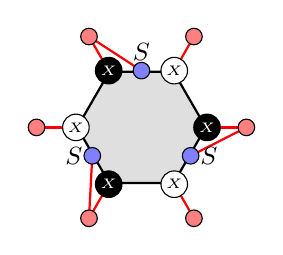
\begin{tikzpicture}
        
        \node[name=g, regular polygon, regular polygon sides = 6, draw, inner sep = 0.5cm, fill=gray, fill opacity=0.25, thick] at (0, 0) {};

        \foreach \anchor/\target/\n in
        {corner 2/side 1/2, corner 4/side 3/4, corner 6/side 5/6}
        {
        \draw[-, red, thick] ($(g.\anchor) + (\n*60:0.5)$) to (g.\target);
        }
        
        \foreach \anchor/\placement/\n/\fill/\text in
        {corner 1/below/1/white/black, corner 2/below/2/black/white, corner 3/right/3/white/black, corner 4/above/4/black/white, corner 5/above/5/white/black, corner 6/left/6/black/white}
        {
        \draw[-, red, thick] ($(g.\anchor) + (\n*60:0.5)$) to (g.\anchor);
        \filldraw[shift=(g.\anchor), fill=red!50!white] (\n*60:0.5) circle (3pt);
        \node[draw, circle, fill=\fill, inner sep = 1pt, text=\text] at (g.\anchor) {\tiny{$X$}};
        }

        \foreach \anchor/\placement in {side 1/above, side 3/left, side 5/right}
        \filldraw[shift=(g.\anchor), fill=blue!50!white] (0,0) circle (3pt) node[\placement] {\small{$S$}};
        
    \end{tikzpicture}
    }
\end{equation}
Here, the red lines joining two degrees of freedom indicate a $CZ$ gate.

Now all of the $S$ support has been moved away from the vertex ancilla onto the edge ancilla, but we have added some new $CZ$ gates.
Using Eq.~\ref{eq:CZ-deformation}, we can push all support on the vertex qubits to a single, root vertex, labeled ``a''. For each vertex ancilla $b \neq a$ touched by a CZ, we find a path $p(a, b)$ between $a$ and $b$. The first identity tells us we can trade a $CZ$ on $b$ for a $CZ$ on $a$ and all the edges along the path $p(a, b)$. To illustrate, let $a$ be the top left vertex ancilla, and $b$ the leftmost ancilla. Then Eq.~\ref{eq:CZ-deformation} gives: 
\begin{equation}
    \raisebox{-45pt}{
    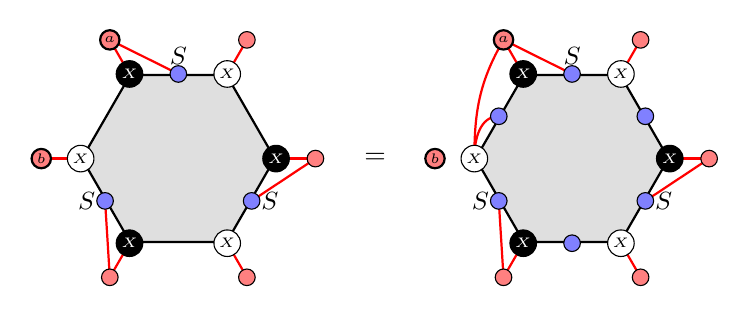
\begin{tikzpicture}[scale=1]
        
        \node[name=g, regular polygon, regular polygon sides = 6, draw, inner sep = 0.75cm, fill=gray, fill opacity=0.25, thick] at (0, 0) {};

       \foreach \anchor/\target/\n in
        {corner 2/side 1/2, corner 4/side 3/4, corner 6/side 5/6}
        {
        \draw[-, red, thick] ($(g.\anchor) + (\n*60:0.5)$) to (g.\target);
        }
        
        \foreach \anchor/\placement/\n/\fill/\text in
        {corner 1/below/1/white/black, corner 2/below/2/black/white, corner 3/right/3/white/black, corner 4/above/4/black/white, corner 5/above/5/white/black, corner 6/left/6/black/white}
        {
        \draw[-, red, thick] ($(g.\anchor) + (\n*60:0.5)$) to (g.\anchor);
        \filldraw[shift=(g.\anchor), fill=red!50!white] (\n*60:0.5) circle (3pt);
        \node[draw, circle, fill=\fill, inner sep = 1pt, text=\text] at (g.\anchor) {\tiny{$X$}};
        }

        \filldraw[shift=(g.corner 2), fill=white!50!red, thick] (2*60:0.5) circle (3.5pt) node[name=v] {\tiny {$a$}};

        \filldraw[shift=(g.corner 3), fill=white!50!red, thick] (3*60:0.5) circle (3.5pt) node[name=v] {\tiny {$b$}};

        \foreach \anchor/\placement in {side 1/above, side 3/left, side 5/right}
        \filldraw[shift=(g.\anchor), fill=blue!50!white] (0,0) circle (3pt) node[\placement] {\small{$S$}};


        \node at (2.5, 0) {$=$};


        \node[name=g, regular polygon, regular polygon sides = 6, draw, inner sep = 0.75cm, fill=gray, fill opacity=0.25, thick] at (5, 0) {};

        \foreach \anchor/\target/\n in
        {corner 2/side 1/2, corner 4/side 3/4, corner 6/side 5/6}
        {
        \draw[-, red, thick] ($(g.\anchor) + (\n*60:0.5)$) to (g.\target);
        }

        \foreach \anchor/\placement/\n/\fill/\text in
        {corner 1/below/1/white/black, corner 2/below/2/black/white, corner 4/above/4/black/white, corner 5/above/5/white/black, corner 6/left/6/black/white}
        {
        \draw[-, red, thick] ($(g.\anchor) + (\n*60:0.5)$) to (g.\anchor);
        }

        \draw[-, red, thick] ($(g.corner 2) + (2*60:0.5)$) to[in=90, out = -120] (g.corner 3);
        \draw[-, red, thick] ($(g.corner 3)$) to[in=180, out=90] (g.side 2);
        
        \foreach \anchor/\placement/\n/\fill/\text in
        {corner 1/below/1/white/black, corner 2/below/2/black/white, corner 3/right/3/white/black, corner 4/above/4/black/white, corner 5/above/5/white/black, corner 6/left/6/black/white}
        {
        \filldraw[shift=(g.\anchor), fill=red!50!white] (\n*60:0.5) circle (3pt);
        \node[draw, circle, fill=\fill, inner sep = 1pt, text=\text] at (g.\anchor) {\tiny{$X$}};
        }

        \filldraw[shift=(g.corner 2), fill=white!50!red, thick] (2*60:0.5) circle (3.5pt) node[name=v] {\tiny {$a$}};

        \filldraw[shift=(g.corner 3), fill=white!50!red, thick] (3*60:0.5) circle (3.5pt) node[name=v] {\tiny {$b$}};

        \foreach \anchor/\placement in {side 1/above, side 3/left, side 5/right}
        \filldraw[shift=(g.\anchor), fill=blue!50!white] (0,0) circle (3pt) node[\placement] {\small{$S$}};

        \foreach \anchor/\placement in {side 2/above, side 4/left, side 6/right}
        \filldraw[shift=(g.\anchor), fill=blue!50!white] (0,0) circle (3pt) node[\placement] {};
        
    \end{tikzpicture}
    }
\end{equation}
We have removed $Z$ support on vertex ancilla $b$ from the stabilizer. We can repeat this process for all the other vertex ancillas (excluding the root, $a$). We obtain the following deformed stabilizer:
\begin{equation}
    \raisebox{-35pt}{
    \begin{tikzpicture}

        \node[name=g, regular polygon, regular polygon sides = 6, draw, inner sep = 0.75cm, fill=gray, fill opacity=0.25, thick] at (0, 0) { };

        \filldraw[shift=(g.corner 2), fill=white!50!red, thick] (-0.5, 0.5) circle (3.5pt) node[name=v] {\tiny {$a$} };

        \foreach \anchor/\placement/\n/\fill/\text/\name in
        {corner 1/below/1/white/black/A, corner 2/below/2/black/white/B, corner 3/right/3/white/black/C, corner 4/above/4/black/white/D, corner 5/above/5/white/black/E, corner 6/left/6/black/white/F}
        {
        \node[draw, circle, fill=\fill, inner sep = 1pt, text=\text, name=\name] at (g.\anchor) {\tiny{$X$}};
        }

        \foreach \anchor/\placement/\name in
        {side 2/left/b, side 4/below/d, side 6/right/f}
        {
        \filldraw[shift=(g.\anchor), fill=blue!50!white, fill opacity = 1, thick] (0,0) circle (4pt);
        \node[name=\name] at (g.\anchor) { }; 
        }

        \foreach \anchor/\placement/\name in
        {side 1/above/a, side 3/left/c, side 5/right/e}
        {
        \filldraw[shift=(g.\anchor), fill=blue!50!white, fill opacity = 1, thick] (0,0) circle (4pt);
        \node[name=\name] at (g.\anchor) {\tiny{$S$}}; 
        }
        
        
        \draw[-, thick, red] (a) to[in=-100, out=-90] (A);
        \draw[-, thick, red] (a) to[in=180, out=-90] (F);
        \draw[-, thick, red] (a) to[in=120, out=-90] (E);

        \draw[-, thick, red] (f) to[in=180, out=-130] (F);
        \draw[-, thick, red] (f) to[in=120, out=-130] (E);

        \draw[-, thick, red] (e) to[in=120, out=170] (E);

        \draw[-, thick, red] (c) to[in=50, out=10] (D);
        
        \draw[-, thick, red] (b) to[in=50, out=-30] (D);
        \draw[-, thick, red] (b) to[in=0, out=-70] (C);

        \draw[-, red, thick] (v) to[in=130, out=10] (A);
        \draw[-, red, thick] (v) to[in=120, out=-30] (B);
        \draw[-, red, thick] (v) to[in=100, out=-110] (C);
        \draw[-, red, thick] (v) to[in=180, out=-160] (D);
        \draw[-, red, thick] (v) to[in=140, out=-90] (E);
        \draw[-, red, thick] (v) to[in=60, out=50] (F);
        \draw[-, red, thick] (v) to[in=90, out=5] (a);
        \draw[-, red, thick] (v) to[in=170, out=220] (c);
        \draw[-, red, thick] (v) to[in=150, out=-70] (e);

        \draw[-, red, thick] (a) to[in=200, out=-90] (f);
        \draw[-, red, thick] (a) to[in=10, out=-90] (c);

        \draw[-, red, thick] (c) to[in=90, out=10] (d);
        \draw[-, red, thick] (c) to[in=150, out=10] (e);
        \draw[-, red, thick] (f) to[in=10, out=-130] (c);
        
        \draw[-, red, thick] (f) to[in=120, out=-130] (e);

        \node at (2.5, 0) {$=$};


        \node[name=g, regular polygon, regular polygon sides = 6, draw, inner sep = 0.75cm, fill=gray, fill opacity=0.25, thick] at (5, 0) { };
        
        \foreach \anchor/\placement/\n/\fill/\text/\name in
        {corner 1/below/1/white/black/A, corner 2/below/2/black/white/B, corner 3/right/3/white/black/C, corner 4/above/4/black/white/D, corner 5/above/5/white/black/E, corner 6/left/6/black/white/F}
        {
        \node[draw, circle, fill=\fill, inner sep = 1pt, text=\text, name=\name] at (g.\anchor) {\tiny{$X$}};
        }

        \foreach \anchor/\placement/\name in
        {side 2/left/b, side 4/below/d, side 6/right/f}
        {
        \filldraw[shift=(g.\anchor), fill=blue!50!white, fill opacity = 1, thick] (0,0) circle (4pt);
        \node[name=\name] at (g.\anchor) { }; 
        }

        \foreach \anchor/\placement/\name in
        {side 1/above/a, side 3/left/c, side 5/right/e}
        {
        \filldraw[shift=(g.\anchor), fill=blue!50!white, fill opacity = 1, thick] (0,0) circle (4pt);
        \node[name=\name] at (g.\anchor) {\tiny{$S$}}; 
        }
        
        \draw[-, thick, red] (a) to[in=-100, out=-90] (A);
        \draw[-, thick, red] (a) to[in=180, out=-90] (F);
        \draw[-, thick, red] (a) to[in=120, out=-90] (E);

        \draw[-, thick, red] (f) to[in=180, out=-130] (F);
        \draw[-, thick, red] (f) to[in=120, out=-130] (E);

        \draw[-, thick, red] (e) to[in=120, out=170] (E);

        \draw[-, thick, red] (c) to[in=50, out=10] (D);
        
        \draw[-, thick, red] (b) to[in=50, out=-30] (D);
        \draw[-, thick, red] (b) to[in=0, out=-70] (C);

        \draw[-, red, thick] (a) to[in=200, out=-90] (f);
        \draw[-, red, thick] (a) to[in=10, out=-90] (c);

        \draw[-, red, thick] (c) to[in=90, out=10] (d);
        \draw[-, red, thick] (c) to[in=150, out=10] (e);
        \draw[-, red, thick] (f) to[in=10, out=-130] (c);
        
        \draw[-, red, thick] (f) to[in=120, out=-130] (e);
        

        \node at (7, 0) {$\times$};
        \node at (7.5, 0) {$C_a$};
        \draw [decorate, decoration = {calligraphic brace}, thick] (8, -1.25) -- (8, 1.25);
        \draw [decorate, decoration = {calligraphic brace, mirror}, thick] (11.5, -1.25) -- (11.5, 1.25);


        \node[name=g, regular polygon, regular polygon sides = 6, draw, inner sep = 0.75cm, fill=gray, fill opacity=0.25, thick] at (9.75, 0) { };

        \foreach \anchor/\placement/\n/\fill/\text/\name in
        {corner 1/below/1/white/black/A, corner 2/below/2/black/white/B, corner 3/right/3/white/black/C, corner 4/above/4/black/white/D, corner 5/above/5/white/black/E, corner 6/left/6/black/white/F}
        {
        \node[draw, circle, fill=\fill, inner sep = 1pt, text=\text, name=\name] at (g.\anchor) {\tiny{$Z$}};
        }

        \foreach \anchor/\placement/\name in
        {side 1/above/a, side 3/left/c, side 5/right/e}
        {
        \filldraw[shift=(g.\anchor), fill=blue!50!white, fill opacity = 1, thick] (0,0) circle (4pt); 
        \node[name=\name] at (g.\anchor) {\tiny{$Z$}};
        }
    \end{tikzpicture}
    }
\end{equation} 
The controlled-stabilizer is trivial on the codespace, and so we can ignore it (with the caveat that the resulting stabilizers will only strictly commute \emph{in the codespace}). Thus, we have removed all support on the vertex qubits that does not commute with the $X$ measurement. The final stabilizers are:
\begin{equation}
    \raisebox{-30pt}{
    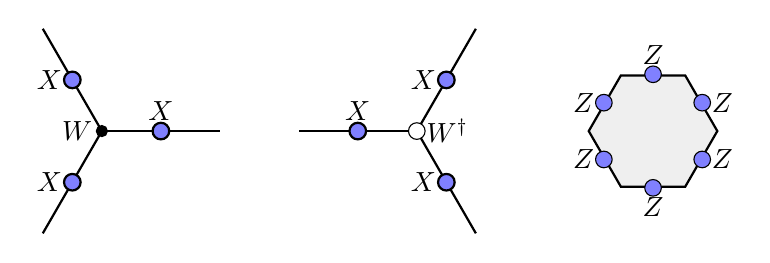
\begin{tikzpicture}
        \filldraw[] (0,0) circle (2pt) node[left] {$W$};
        \draw[-, thick] (0, 0) -- (1.5, 0);
        \draw[-, thick] (0, 0) -- (120:1.5);
        \draw[-, thick] (0, 0) -- (240:1.5);

        \filldraw[fill=blue!50!white, thick] (0:0.75) circle (3pt) node[above] {$X$};
        \filldraw[fill=blue!50!white, thick] (120:0.75) circle (3pt) node[left] {$X$};
        \filldraw[fill=blue!50!white, thick] (240:0.75) circle (3pt) node[left] {$X$};

        
        \draw[-, thick] (4, 0) -- (2.5, 0);
        \draw[-, thick] (4, 0) -- ($(4, 0) + (60:1.5)$);
        \draw[-, thick] (4, 0) -- ($(4, 0) + (300:1.5)$);
        \filldraw[fill=white] (4,0) circle (3pt) node[right] {$W^\dagger$};

        \filldraw[fill=blue!50!white, thick] ($(4, 0) + (180:0.75)$) circle (3pt) node[above] {$X$};
        \filldraw[fill=blue!50!white, thick] ($(4, 0) + (60:0.75)$) circle (3pt) node[left] {$X$};
        \filldraw[fill=blue!50!white, thick] ($(4, 0) + (300:0.75)$) circle (3pt) node[left] {$X$};


        \node[name = h, regular polygon, regular polygon sides = 6, draw, inner sep = 0.5cm, fill=gray!50!white, fill opacity=0.25, thick] at (7, 0) {};
        \foreach \anchor/\placement in
        {side 1/above, side 2/left, side 3/left, side 4/below, side 5/right, side 6/right}
        {
        \filldraw[shift=(h.\anchor), fill=blue!50!white] (0,0) circle (3pt) node[\placement] {$Z$};
        }
    \end{tikzpicture}
    }
\end{equation}
\begin{equation}
    \raisebox{-30pt}{
    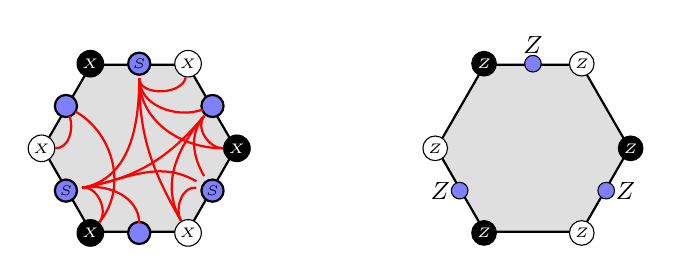
\begin{tikzpicture}
        \node[name=g, regular polygon, regular polygon sides = 6, draw, inner sep = 0.75cm, fill=gray, fill opacity=0.25, thick] at (0, 0) { };
        
        \foreach \anchor/\placement/\n/\fill/\text/\name in
        {corner 1/below/1/white/black/A, corner 2/below/2/black/white/B, corner 3/right/3/white/black/C, corner 4/above/4/black/white/D, corner 5/above/5/white/black/E, corner 6/left/6/black/white/F}
        {
        \node[draw, circle, fill=\fill, inner sep = 1pt, text=\text, name=\name] at (g.\anchor) {\tiny{$X$}};
        }

        \foreach \anchor/\placement/\name in
        {side 2/left/b, side 4/below/d, side 6/right/f}
        {
        \filldraw[shift=(g.\anchor), fill=blue!50!white, fill opacity = 1, thick] (0,0) circle (4pt);
        \node[name=\name] at (g.\anchor) { }; 
        }

        \foreach \anchor/\placement/\name in
        {side 1/above/a, side 3/left/c, side 5/right/e}
        {
        \filldraw[shift=(g.\anchor), fill=blue!50!white, fill opacity = 1, thick] (0,0) circle (4pt);
        \node[name=\name] at (g.\anchor) {\tiny{$S$}}; 
        }
        
        \draw[-, thick, red] (a) to[in=-100, out=-90] (A);
        \draw[-, thick, red] (a) to[in=180, out=-90] (F);
        \draw[-, thick, red] (a) to[in=120, out=-90] (E);

        \draw[-, thick, red] (f) to[in=180, out=-130] (F);
        \draw[-, thick, red] (f) to[in=120, out=-130] (E);

        \draw[-, thick, red] (e) to[in=120, out=170] (E);

        \draw[-, thick, red] (c) to[in=50, out=10] (D);
        
        \draw[-, thick, red] (b) to[in=50, out=-30] (D);
        \draw[-, thick, red] (b) to[in=0, out=-70] (C);

        \draw[-, red, thick] (a) to[in=200, out=-90] (f);
        \draw[-, red, thick] (a) to[in=10, out=-90] (c);

        \draw[-, red, thick] (c) to[in=90, out=10] (d);
        \draw[-, red, thick] (c) to[in=150, out=10] (e);
        \draw[-, red, thick] (f) to[in=10, out=-130] (c);
        
        \draw[-, red, thick] (f) to[in=120, out=-130] (e);


        \node[name=g, regular polygon, regular polygon sides = 6, draw, inner sep = 0.75cm, fill=gray, fill opacity=0.25, thick] at (5, 0) {};
        
        \foreach \anchor/\placement/\n/\fill/\text in
        {corner 1/below/1/white/black, corner 2/below/2/black/white, corner 3/right/3/white/black, corner 4/above/4/black/white, corner 5/above/5/white/black, corner 6/left/6/black/white}
        {
        \node[draw, circle, fill=\fill, inner sep = 1pt, text=\text] at (g.\anchor) {\tiny{$Z$}};
        }

        \foreach \anchor/\placement in {side 1/above, side 3/left, side 5/right}
        \filldraw[shift=(g.\anchor), fill=blue!50!white] (0,0) circle (3pt) node[\placement] {\small{$Z$}};
        
    \end{tikzpicture}
    }
\end{equation}
We note that the deformed $X$ hexagon has a large number of $CZ$ gates, and so would be rather impractical to measure in an actual device. Different choices of vertex set lead to different decorations on the original code stabilizers, which may be more or less tractable; thus the choice of vertex set is an important choice that should be taken into consideration when designing a Clifford measurement scheme for practical use.

\subsubsection{Unit Cell per Vertex Set}
The procedure to generate the stabilizers is the same as the previous example, but now we partition the transversal $XS$ symmetry by unit cells of the honeycomb lattice, rather than by individual sites. A vertex set  consists of two neighboring $A, B$ sites--- we choose sites connected by a flat, horizontal edge.

After the symmetry enrichment, the stabilizers are given by:
\begin{equation}
    \raisebox{-45pt}{
    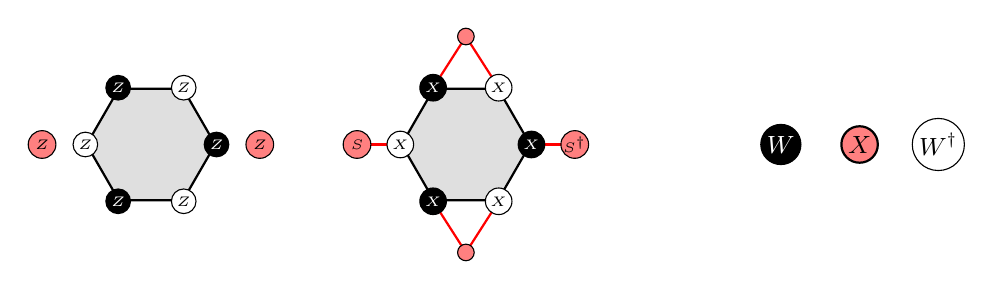
\begin{tikzpicture}

        \node[name=g, regular polygon, regular polygon sides = 6, draw, inner sep = 0.5cm, fill=gray, fill opacity=0.25, thick] at (-4, 0) {};

        \filldraw[shift=(g.corner 3), fill=red!50!white] (180:0.55) circle (5pt);
        \node[inner sep = 1pt] at ($(g.corner 3) + (180:0.55)$) {\tiny{$Z$}};

        \filldraw[shift=(g.corner 6), fill=red!50!white] (0:0.55) circle (5pt);
        \node[inner sep = 1pt] at ($(g.corner 6) + (0:0.55)$) {\tiny{$Z$}};
        
        \foreach \anchor/\placement/\n/\fill/\text in
        {corner 1/below/1/white/black, corner 2/below/2/black/white, corner 3/right/3/white/black, corner 4/above/4/black/white, corner 5/above/5/white/black, corner 6/left/6/black/white}
        {
        \node[draw, circle, fill=\fill, inner sep = 1pt, text=\text] at (g.\anchor) {\tiny{$Z$}};
        }


        \node[name=g, regular polygon, regular polygon sides = 6, draw, inner sep = 0.5cm, fill=gray, fill opacity=0.25, thick] at (0, 0) {};

        \draw[-, red, thick] ($(g.corner 3) + (180:0.55)$) to (g.corner 3);
        \filldraw[shift=(g.corner 3), fill=red!50!white] (180:0.55) circle (5pt);
        \node[inner sep = 1pt] at ($(g.corner 3) + (180:0.55)$) {\tiny{$S$}};

        \draw[-, red, thick] ($(g.corner 6) + (0:0.55)$) to (g.corner 6);
        \filldraw[shift=(g.corner 6), fill=red!50!white] (0:0.55) circle (5pt);
        \node[inner sep = 1pt] at ($(g.corner 6) + (0:0.55)$) {\tiny{$S^\dagger$}};

        \draw[-, red, thick] (g.corner 1) to ($(g.side 1) + (0, 0.65)$);
        \draw[-, red, thick] (g.corner 2) to ($(g.side 1) + (0, 0.65)$);
        \filldraw[shift=(g.side 1), fill=red!50!white] (0, 0.65) circle (3pt);

        \draw[-, red, thick] (g.corner 4) to ($(g.side 4) + (0, -0.65)$);
        \draw[-, red, thick] (g.corner 5) to ($(g.side 4) + (0, -0.65)$);
        \filldraw[shift=(g.side 4), fill=red!50!white] (0, -0.65) circle (3pt);
        
        \foreach \anchor/\placement/\n/\fill/\text in
        {corner 1/below/1/white/black, corner 2/below/2/black/white, corner 3/right/3/white/black, corner 4/above/4/black/white, corner 5/above/5/white/black, corner 6/left/6/black/white}
        {
        \node[draw, circle, fill=\fill, inner sep = 1pt, text=\text] at (g.\anchor) {\tiny{$X$}};
        }


        \node[shape=circle, fill=red!50!white, draw, thick, inner sep=1pt] at (5, 0) {\small{$X$}};
        \node[shape=circle, fill=black, text=white, draw, inner sep=1pt] at (4, 0) {\small{$W$}};
        \node[shape=circle, fill=white, text=black, draw, inner sep=1pt] at (6, 0) {\small{$W^\dagger$}};
        
    \end{tikzpicture}
    }
\end{equation}
Again, we introduce edge ancilla and entangle with the vertex ancilla in a cluster state. Here, the convenient choice is a square lattice defined by our choice of unit cells. The resultant stabilizers are
\begin{equation}
    \raisebox{-35pt}{
    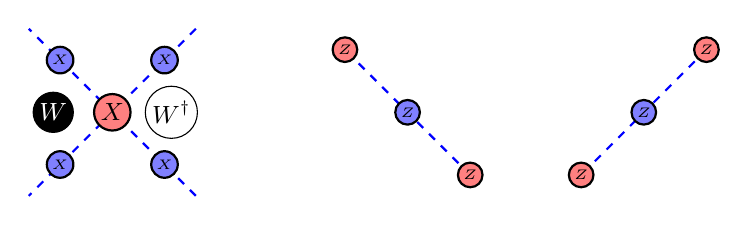
\begin{tikzpicture}[scale=0.75]


        \draw[-, dashed, thick, blue] ($(5,0) + (-45:2)$) -- ($(5, 0) + (135:2)$);
        \draw[-, dashed, thick, blue] ($(5,0) + (45:2)$) -- ($(5, 0) + (225:2)$);

        \node[shape=circle, fill=blue!50!white, draw, thick, inner sep=1pt] at ($(5,0) + (45:1.25)$) {\tiny{$X$}};
        \node[shape=circle, fill=blue!50!white, draw, thick, inner sep=1pt] at ($(5,0) + (-45:1.25)$) {\tiny{$X$}};
        \node[shape=circle, fill=blue!50!white, draw, thick, inner sep=1pt] at ($(5,0) + (135:1.25)$) {\tiny{$X$}};
        \node[shape=circle, fill=blue!50!white, draw, thick, inner sep=1pt] at ($(5,0) + (225:1.25)$) {\tiny{$X$}};
        
        \node[shape=circle, fill=red!50!white, draw, thick, inner sep=1pt] at (5, 0) {\small{$X$}};
        \node[shape=circle, fill=black, text=white, draw, inner sep=1pt] at (4, 0) {\small{$W$}};
        \node[shape=circle, fill=white, text=black, draw, inner sep=1pt] at (6, 0) {\small{$W^\dagger$}};


        \draw[-, dashed, thick, blue] ($(10,0) + (-45:1.5)$) -- ($(10, 0) + (135:1.5)$);
        \node[shape=circle, fill=blue!50!white, draw, thick, inner sep=1pt] at (10, 0) {\tiny{$Z$}};
        
        \node[shape=circle, fill=red!50!white, draw, thick, inner sep=1pt] at ($(10, 0) + (-45:1.5)$) {\tiny{$Z$}};
        \node[shape=circle, fill=red!50!white, draw, thick, inner sep=1pt] at ($(10, 0) + (135:1.5)$) {\tiny{$Z$}};


        \draw[-, dashed, thick, blue] ($(14,0) + (45:1.5)$) -- ($(14, 0) + (-135:1.5)$);
        \node[shape=circle, fill=blue!50!white, draw, thick, inner sep=1pt] at (14, 0) {\tiny{$Z$}};
        
        \node[shape=circle, fill=red!50!white, draw, thick, inner sep=1pt] at ($(14, 0) + (45:1.5)$) {\tiny{$Z$}};
        \node[shape=circle, fill=red!50!white, draw, thick, inner sep=1pt] at ($(14, 0) + (-135:1.5)$) {\tiny{$Z$}};
        
    \end{tikzpicture}
    }
\end{equation}

Again, we need to project the vertices onto the $X$ basis, and so need to get rid of any support on the vertices that does not commute with this measurement. We use the same identities as the previous example. The $Z$ hexagon, $A_v$, and $B_p$ terms are straightforward:

\begin{equation}
    \raisebox{-45pt}{
    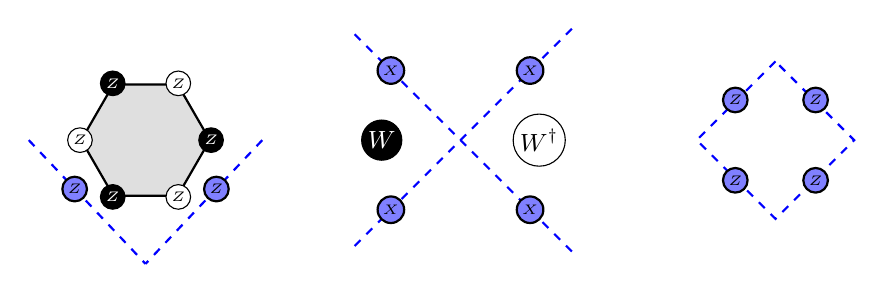
\begin{tikzpicture}

        \node[name=g, regular polygon, regular polygon sides = 6, draw, inner sep = 0.5cm, fill=gray, fill opacity=0.25, thick] at (-4, 0) {};

        \draw[-, dashed, blue, thick] ($(g.corner 3) + (180:0.65)$) -- ($(g.side 4) + (0, -0.85)$);
        \draw[-, dashed, blue, thick] ($(g.corner 6) + (0:0.65)$) -- ($(g.side 4) + (0, -0.85)$);
        \node[shape=circle, fill=blue!50!white, draw, thick, inner sep=1pt] at ($(g.side 4) + (-0.9, 0.1)$) {\tiny{$Z$}};
        \node[shape=circle, fill=blue!50!white, draw, thick, inner sep=1pt] at ($(g.side 4) + (0.9, 0.1)$) {\tiny{$Z$}};
        
        
        \foreach \anchor/\placement/\n/\fill/\text in
        {corner 1/below/1/white/black, corner 2/below/2/black/white, corner 3/right/3/white/black, corner 4/above/4/black/white, corner 5/above/5/white/black, corner 6/left/6/black/white}
        {
        \node[draw, circle, fill=\fill, inner sep = 1pt, text=\text] at (g.\anchor) {\tiny{$Z$}};
        }


        \draw[-, dashed, thick, blue] ($(0,0) + (-45:2)$) -- ($(0, 0) + (135:2)$);
        \draw[-, dashed, thick, blue] ($(0,0) + (45:2)$) -- ($(0, 0) + (225:2)$);

        \node[shape=circle, fill=blue!50!white, draw, thick, inner sep=1pt] at ($(0,0) + (45:1.25)$) {\tiny{$X$}};
        \node[shape=circle, fill=blue!50!white, draw, thick, inner sep=1pt] at ($(0,0) + (-45:1.25)$) {\tiny{$X$}};
        \node[shape=circle, fill=blue!50!white, draw, thick, inner sep=1pt] at ($(0,0) + (135:1.25)$) {\tiny{$X$}};
        \node[shape=circle, fill=blue!50!white, draw, thick, inner sep=1pt] at ($(0,0) + (225:1.25)$) {\tiny{$X$}};
        
        \node[shape=circle, fill=black, text=white, draw, inner sep=1pt] at (-1, 0) {\small{$W$}};
        \node[shape=circle, fill=white, text=black, draw, inner sep=1pt] at (1, 0) {\small{$W^\dagger$}};
        

        \node[name= g, regular polygon, regular polygon sides = 4, inner sep = 0.5cm, rotate=45, draw, blue, thick, dashed] at (4, 0) {};

        \foreach \anchor in 
        {side 1, side 2, side 3, side 4}
        {
        \node[shape=circle, fill=blue!50!white, draw, thick, inner sep=1pt] at (g.\anchor) {\tiny{$Z$}};
        }
        
    \end{tikzpicture}
    }
\end{equation}

The $X$ hexagon is modified as follows (again using Eqs.~\ref{eq:CZ-deformation} and \ref{eq:S-deformation}, with the topmost vertex as the root):
\begin{equation}
    \raisebox{-45pt}{
    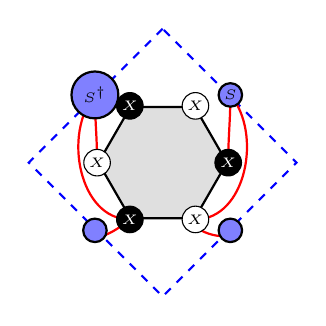
\begin{tikzpicture}

        \node[name=g, regular polygon, regular polygon sides = 6, draw, inner sep = 0.5cm, fill=gray, fill opacity=0.25, thick] at (-4, 0) {};

        \node[name=s, regular polygon, regular polygon sides = 4, rotate= 45, inner sep = 0.85cm, draw, blue, dashed, thick] at (-4, 0) {};

        \draw[-, red, thick] (s.side 1) to[in=90, out=-90] (g.corner 3);
        \draw[-, red, thick] (s.side 1) to[in=180, out=230] (g.corner 4);

        \draw[-, red, thick] (s.side 4) to[in=0, out=-50] (g.corner 5);
        \draw[-, red, thick] (s.side 4) to[in=90, out=-90] (g.corner 6);

        \draw[-, red, thick] (s.side 2) to[in=220, out=-90] (g.corner 4);

        \draw[-, red, thick] (s.side 3) to[in=220, out=-90] (g.corner 5);
        
        \foreach \anchor/\placement/\n/\fill/\text in
        {corner 1/below/1/white/black, corner 2/below/2/black/white, corner 3/right/3/white/black, corner 4/above/4/black/white, corner 5/above/5/white/black, corner 6/left/6/black/white}
        {
        \node[draw, circle, fill=\fill, inner sep = 1pt, text=\text] at (g.\anchor) {\tiny{$X$}};
        }

        
        \node[shape=circle, fill=blue!50!white, draw, thick, inner sep=2.5pt] at (s.side 1) {\tiny{$S^\dagger$}};
        \node[shape=circle, fill=blue!50!white, draw, thick, inner sep=1pt] at (s.side 4) {\tiny{$S$}};
        \node[shape=circle, fill=blue!50!white, draw, thick, inner sep=3pt] at (s.side 2) {};
        \node[shape=circle, fill=blue!50!white, draw, thick, inner sep=3pt] at (s.side 3) {};

    \end{tikzpicture}
    }
\end{equation}


\subsubsection{Hexagon per Vertex Set}

For the last part of this example, we assign a three-coloring to the honeycomb lattice. Each hexagonal face of the lattice is assigned red, blue, or green, and no hexagon of the same color may share a site. Hexagons of a single color (say, green) thus form a partition of the lattice, and a convenient choice of vertex set. 

We introduce a new ancilla qubit for every vertex set, initialized in the $\ket{+}$ state, and we entangle it with its vertex set by applying $CW$/$C\tilde{W}$ gates with the ancilla as the control. The new stabilizers of the model are as follows: 
\begin{equation}
    \raisebox{-35pt}{
    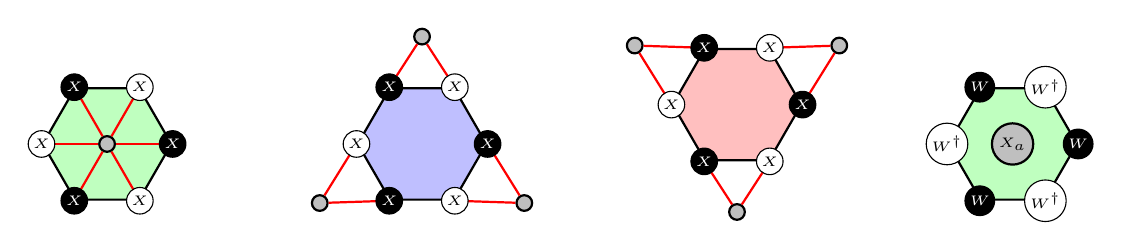
\begin{tikzpicture}

        \node[name=g, regular polygon, regular polygon sides = 6, draw, inner sep = 0.5cm, fill=green, fill opacity=0.25, thick] at (0, 0) {};
        \node[shape=circle, fill=gray!50!white, draw, thick, inner sep=2pt, name=ga] at (g.center) { };
        
        \foreach \anchor/\placement/\n/\fill/\text/\op in
        {corner 1/below/1/white/black, corner 2/below/2/black/white, corner 3/right/3/white/black, corner 4/above/4/black/white, corner 5/above/5/white/black, corner 6/left/6/black/white}
        {
        \draw[-, red, thick] (ga) to (g.\anchor);
        \node[draw, circle, fill=\fill, inner sep = 1pt, text=\text] at (g.\anchor) {\tiny{$X$}};
        }

        
        \node[name= b, regular polygon, regular polygon sides = 6, draw, inner sep = 0.5cm, fill=blue, fill opacity=0.25, thick] at (4, 0) {};
        
        \node at (b.center) [shape=circle, fill=gray!50!white, draw, thick, inner sep=2pt, name=ba,  above=1.25cm] { };
        \node [shape=circle, fill=gray!50!white, draw, thick, inner sep=2pt, name=bb] at ($ (1.299, -0.75) + (b.center) $) { };
        \node [shape=circle, fill=gray!50!white, draw, thick, inner sep=2pt, name=bc] at ($ (-1.299, -0.75) + (b.center) $) { };

        \draw[-, red, thick] (ba) to (b.corner 1);
        \draw[-, red, thick] (ba) to (b.corner 2);

        \draw[-, red, thick] (bb) to (b.corner 6);
        \draw[-, red, thick] (bb) to (b.corner 5);

        \draw[-, red, thick] (bc) to (b.corner 4);
        \draw[-, red, thick] (bc) to (b.corner 3);

       \foreach \anchor/\placement/\n/\fill/\text/\op in
        {corner 1/below/1/white/black, corner 2/below/2/black/white, corner 3/right/3/white/black, corner 4/above/4/black/white, corner 5/above/5/white/black, corner 6/left/6/black/white}
        {
        \node[draw, circle, fill=\fill, inner sep = 1pt, text=\text] at (b.\anchor) {\tiny{$X$}};
        }
        


        \node[name = r, regular polygon, regular polygon sides = 6, draw, inner sep = 0.5cm, fill=red, fill opacity=0.25, thick] at (8, 0.5) {};
        \node at (r.center) [shape=circle, fill=gray!50!white, draw, thick, inner sep=2pt, name=ra,  below=1.25cm] { };
        \node [shape=circle, fill=gray!50!white, draw, thick, inner sep=2pt, name=rb] at ($ (-1.299, 0.75) + (r.center) $) { };
        \node [shape=circle, fill=gray!50!white, draw, thick, inner sep=2pt, name=rc] at ($ (1.299, 0.75) + (r.center) $) { };

        \draw[-, red, thick] (ra) to (r.corner 5);
        \draw[-, red, thick] (ra) to (r.corner 4);

        \draw[-, red, thick] (rb) to (r.corner 3);
        \draw[-, red, thick] (rb) to (r.corner 2);

        \draw[-, red, thick] (rc) to (r.corner 6);
        \draw[-, red, thick] (rc) to (r.corner 1);
        
        \foreach \anchor/\placement/\n/\fill/\text/\op in
        {corner 1/below/1/white/black, corner 2/below/2/black/white, corner 3/right/3/white/black, corner 4/above/4/black/white, corner 5/above/5/white/black, corner 6/left/6/black/white}
        {
        \node[draw, circle, fill=\fill, inner sep = 1pt, text=\text] at (r.\anchor) {\tiny{$X$}};
        }


        \node[name = g2, regular polygon, regular polygon sides = 6, draw, inner sep = 0.5cm, fill=green, fill opacity=0.25, thick] at (11.5, 0) {};
        \node[shape=circle, fill=gray!50!white, draw, thick, inner sep=1.5pt, name=g2a] at (g2.center) {\tiny{$X_a$ }};
        
        \foreach \anchor/\placement/\n/\fill/\text/\op in
        {corner 1/below/1/white/black/$W^\dagger$, corner 2/below/2/black/white/$W$, corner 3/right/3/white/black/$W^\dagger$, corner 4/above/4/black/white/$W$, corner 5/above/5/white/black/$W^\dagger$, corner 6/left/6/black/white/$W$}
        {
        \node[draw, circle, fill=\fill, inner sep = 1pt, text=\text] at (g2.\anchor) {\tiny{\op}};
        }
        
    \end{tikzpicture}
    }
\end{equation}
Here, the vertex ancillas are pictured in grey.

We now introduce edge ancillas, which in this case are placed on all green edges (the edges forming the triangular sublattice defined by the vertex set ancillas). The new edge ancillas are entangled with the vertex ancillas using the CSS cluster entangler.
\begin{equation}
    \raisebox{-45pt}{
    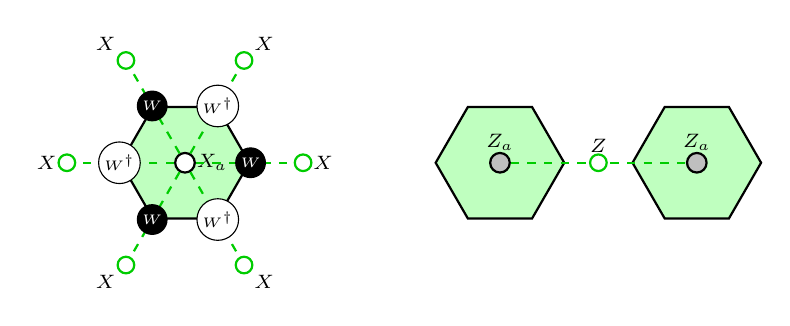
\begin{tikzpicture}
        \node[name = g2, regular polygon, regular polygon sides = 6, draw, inner sep = 0.5cm, fill=green, fill opacity=0.25, thick] at (0, 0) {};
        \node[shape=circle, fill=white, draw, thick, inner sep=2.5pt, name=g2a] at (g2.center) { };
        \node[right, outer sep=1pt] at (g2.center) {\scriptsize\texttt{$X_a$}};

        \foreach \n/\placement in {0/right, 1/above right, 2/above left, 3/left, 4/below left, 5/below right}
        {
        \draw[dashed, thick, green!80!black] (g2a) to (\n*60:1.5);
        \filldraw[shift=(g2.center), fill=white, draw = green!80!black, thick] (\n*60:1.5) circle (3pt) node[\placement] {\scriptsize\texttt{$X$}};
        }
        
        \foreach \anchor/\placement/\n/\fill/\text/\op in
        {corner 1/below/1/white/black/$W^\dagger$, corner 2/below/2/black/white/$W$, corner 3/right/3/white/black/$W^\dagger$, corner 4/above/4/black/white/$W$, corner 5/above/5/white/black/$W^\dagger$, corner 6/left/6/black/white/$W$}
        {
        \node[draw, circle, fill=\fill, inner sep = 1pt, text=\text] at (g2.\anchor) {\tiny{\op}};
        }


        \node[name = g0, regular polygon, regular polygon sides = 6, draw, inner sep = 0.5cm, fill=green, fill opacity=0.25, thick] at (4, 0) {};
        \node[shape=circle, fill=gray!50!white, draw, thick, inner sep=2.5pt, name=g0a] at (g0.center) { };
        \node[above, outer sep=1pt] at (g0.center) {\scriptsize\texttt{$Z_a$}};

        \node[name = g1, regular polygon, regular polygon sides = 6, draw, inner sep = 0.5cm, fill=green, fill opacity=0.25, thick] at (8.5-2, 0) {};
        \node[shape=circle, fill=gray!50!white, draw, thick, inner sep=2.5pt, name=g1a] at (g1.center) { };
        \node[above, outer sep=1pt] at (g1.center) {\scriptsize\texttt{$Z_a$}};

        \draw[dashed, thick, green!80!black] (g0a) to (g1a);
        \filldraw[shift=(g0a.center), fill=white, draw = green!80!black, thick] (0:1.25) circle (3pt) node[above] {\scriptsize\texttt{$Z$}};

        
    \end{tikzpicture}
    }
\end{equation}

We can again pull a controlled-stabilizer out of the deformed stabilizers we currently have:
\begin{equation}
    \raisebox{-75pt}{
    \begin{tikzpicture}
        \node[name=g, regular polygon, regular polygon sides = 6, draw, inner sep = 0.5cm, fill=green, fill opacity=0.25, thick] at (0, 0) {};
        \node[shape=circle, fill=gray!50!white, draw, thick, inner sep=1.5pt, name=ga] at (g.center) { \tiny{$Z_a$}};
        
        \foreach \anchor/\placement/\n/\fill/\text/\op in
        {corner 1/below/1/white/black, corner 2/below/2/black/white, corner 3/right/3/white/black, corner 4/above/4/black/white, corner 5/above/5/white/black, corner 6/left/6/black/white}
        {
        \draw[-, red, thick] (ga) to (g.\anchor);
        \node[draw, circle, fill=\fill, inner sep = 1pt, text=\text] at (g.\anchor) {\tiny{$X$}};
        }

        \node at (2, 0) {$=$};

        \node[name=g2, regular polygon, regular polygon sides = 6, draw, inner sep = 0.5cm, fill=green, fill opacity=0.25, thick] at (4, 0) {};
        \node[shape=circle, fill=gray!50!white, draw, thick, inner sep=1.5pt, name=g2a] at (g2.center) { \tiny{$a$}};
        
        \foreach \anchor/\placement/\n/\fill/\text/\op in
        {corner 1/below/1/white/black, corner 2/below/2/black/white, corner 3/right/3/white/black, corner 4/above/4/black/white, corner 5/above/5/white/black, corner 6/left/6/black/white}
        {
        \node[draw, circle, fill=\fill, inner sep = 1pt, text=\text] at (g2.\anchor) {\tiny{$X$}};
        }
        
        \node at (5.75, 0) {$\times$};
        \node at (6.5, 0) {$C_a$};

        \draw [decorate, decoration = {calligraphic brace}, thick] (7, -1.25) -- (7, 1.25);
        \draw [decorate, decoration = {calligraphic brace, mirror}, thick] (10, -1.25) -- (10, 1.25);


        \node[name=g3, regular polygon, regular polygon sides = 6, draw, inner sep = 0.5cm, fill=green, fill opacity=0.25, thick] at (8.5, 0) {};
        \node[shape=circle, fill=gray!50!white, draw, thick, inner sep=2.5pt, name=g3a] at (g3.center) { \tiny{$a$}};
        \foreach \anchor/\placement/\n/\fill/\text/\op in
        {corner 1/below/1/white/black, corner 2/below/2/black/white, corner 3/right/3/white/black, corner 4/above/4/black/white, corner 5/above/5/white/black, corner 6/left/6/black/white}
        {
        \node[draw, circle, fill=\fill, inner sep = 1pt, text=\text] at (g3.\anchor) {\tiny{$Z$}};
        }


        \node at (2, -3) {$=$};

        \node[name=g2, regular polygon, regular polygon sides = 6, draw, inner sep = 0.5cm, fill=green, fill opacity=0.25, thick] at (4, -3) {};
        \node[shape=circle, fill=gray!50!white, draw, thick, inner sep=2.5pt, name=g2a] at (g2.center) { \tiny{$a$}};
        
        \foreach \anchor/\placement/\n/\fill/\text/\op in
        {corner 1/below/1/white/black, corner 2/below/2/black/white, corner 3/right/3/white/black, corner 4/above/4/black/white, corner 5/above/5/white/black, corner 6/left/6/black/white}
        {
        \node[draw, circle, fill=\fill, inner sep = 1pt, text=\text] at (g2.\anchor) {\tiny{$X$}};
        }

        \node at (9, -3) {(in the color code ground state manifold)};
        
    \end{tikzpicture}
    }
\end{equation}

\begin{equation}
    \raisebox{-90pt}{
    \begin{tikzpicture}
        
        \node[name= b, regular polygon, regular polygon sides = 6, draw, inner sep = 0.5cm, fill=blue, fill opacity=0.25, thick] at (0, 0) {};
        \draw[-, green!80!black, very thick] (b.corner 2) -- (b.corner 3);
        \draw[-, green!80!black, very thick] (b.corner 4) -- (b.corner 5);
        \draw[-, green!80!black, very thick] (b.corner 6) -- (b.corner 1);

        \filldraw[fill=white, draw = green!80!black, thick] (b.side 2) circle (3pt);
        \filldraw[fill=white, draw = green!80!black, thick] (b.side 4) circle (3pt);
        \filldraw[fill=white, draw = green!80!black, thick] (b.side 6) circle (3pt);
        
        \node at (b.center) [shape=circle, fill=white!50!gray, draw, thick, inner sep=1.5pt, name=ba,  above=1.25cm] {\tiny{$Z_a$}};
        \node [shape=circle, fill=white!50!gray, draw, thick, inner sep=1.5pt, name=bb] at ($ (1.299, -0.75) + (b.center) $) {\tiny{$Z_b$}};
        \node [shape=circle, fill=white!50!gray, draw, thick, inner sep=1.5pt, name=bc] at ($ (-1.299, -0.75) + (b.center) $) {\tiny{$Z_c$}};

        \draw[-, red, thick] (ba) to (b.corner 1);
        \draw[-, red, thick] (ba) to (b.corner 2);

        \draw[-, red, thick] (bb) to (b.corner 6);
        \draw[-, red, thick] (bb) to (b.corner 5);

        \draw[-, red, thick] (bc) to (b.corner 4);
        \draw[-, red, thick] (bc) to (b.corner 3);

        \foreach \anchor/\placement/\n/\fill/\text/\op in
        {corner 1/below/1/white/black, corner 2/below/2/black/white, corner 3/right/3/white/black, corner 4/above/4/black/white, corner 5/above/5/white/black, corner 6/left/6/black/white}
        {
        \node[draw, circle, fill=\fill, inner sep = 1pt, text=\text] at (b.\anchor) {\tiny{$X$}};
        }
        

        \node at (2.25, 0) {$=$};

        
        \node[name= b2, regular polygon, regular polygon sides = 6, draw, inner sep = 0.5cm, fill=blue, fill opacity=0.25, thick] at (4.75, 0) {};

        \node at (b2.center) [shape=circle, fill=white!50!gray, draw, thick, inner sep=1.5pt, name=b2a,  above=1.25cm] {\tiny{$Z_a$}};
        \node [shape=circle, fill=white!50!gray, draw, thick, inner sep=1.5pt, name=b2b] at ($ (1.299, -0.75) + (b2.center) $) {\tiny{$Z_b$}};
        \node [shape=circle, fill=white!50!gray, draw, thick, inner sep=1.5pt, name=b2c] at ($ (-1.299, -0.75) + (b2.center) $) {\tiny{$Z_c$}};

        \draw[-, red, thick] (b2a) to (b2.corner 1);
        \draw[-, red, thick] (b2a) to (b2.corner 2);
        \draw[-, red, thick] (b2a) to[out=180, in=180] (b2.corner 3);
        \draw[-, red, thick] (b2a) to[out=180, in=180] (b2.corner 4);
        \draw[-, red, thick] (b2a) to[out=0, in=0] (b2.corner 5);
        \draw[-, red, thick] (b2a) to[out=0, in=0] (b2.corner 6);

        \draw[-, red, thick] (b2.side 6) to[out=180, in=200] (b2.corner 6);
        \draw[-, red, thick] (b2.side 6) to[out=180, in=120] (b2.corner 5);

        \draw[-, red, thick] (b2.side 2) to[out=0, in=0] (b2.corner 3);
        \draw[-, red, thick] (b2.side 2) to[out=0, in=60] (b2.corner 4);
        
        
        \draw[-, green!80!black, very thick] (b2.corner 2) -- (b2.corner 3);
        \draw[-, green!80!black, very thick] (b2.corner 4) -- (b2.corner 5);
        \draw[-, green!80!black, very thick] (b2.corner 6) -- (b2.corner 1);

        \filldraw[fill=white, draw = green!80!black, thick] (b2.side 2) circle (3pt);
        \filldraw[fill=white, draw = green!80!black, thick] (b2.side 4) circle (3pt);
        \filldraw[fill=white, draw = green!80!black, thick] (b2.side 6) circle (3pt);

        \foreach \anchor/\placement/\n/\fill/\text/\op in
        {corner 1/below/1/white/black, corner 2/below/2/black/white, corner 3/right/3/white/black, corner 4/above/4/black/white, corner 5/above/5/white/black, corner 6/left/6/black/white}
        {
        \node[draw, circle, fill=\fill, inner sep = 1pt, text=\text] at (b2.\anchor) {\tiny{$X$}};
        }


        \node at (0, -3) {$=$};

        
        \node[name= b3, regular polygon, regular polygon sides = 6, draw, inner sep = 0.5cm, fill=blue, fill opacity=0.25, thick] at (3.75-2, -3) {};

        \draw[-, red, thick] (b3.side 6) to[out=180, in=200] (b3.corner 6);
        \draw[-, red, thick] (b3.side 6) to[out=180, in=120] (b3.corner 5);

        \draw[-, red, thick] (b3.side 2) to[out=0, in=0] (b3.corner 3);
        \draw[-, red, thick] (b3.side 2) to[out=0, in=60] (b3.corner 4);
        
        \draw[-, green!80!black, very thick] (b3.corner 2) -- (b3.corner 3);
        \draw[-, green!80!black, very thick] (b3.corner 4) -- (b3.corner 5);
        \draw[-, green!80!black, very thick] (b3.corner 6) -- (b3.corner 1);

        \filldraw[fill=white, draw = green!80!black, thick] (b3.side 2) circle (3pt) node {\tiny{$\beta$}};
        \filldraw[fill=white, draw = green!80!black, thick] (b3.side 4) circle (3pt) node {\tiny{$\alpha$}};
        \filldraw[fill=white, draw = green!80!black, thick] (b3.side 6) circle (3pt) node {\tiny{$\gamma$}};

        \foreach \anchor/\placement/\n/\fill/\text/\op in
        {corner 1/below/1/white/black, corner 2/below/2/black/white, corner 3/right/3/white/black, corner 4/above/4/black/white, corner 5/above/5/white/black, corner 6/left/6/black/white}
        {
        \node[draw, circle, fill=\fill, inner sep = 1pt, text=\text] at (b3.\anchor) {\tiny{$X$}};
        }

        \node at (b3.center) [shape=circle, fill=white!50!gray, draw, thick, inner sep=1.5pt, name=b3a,  above=1.25cm] {\tiny{$a$}};
        \node [shape=circle, fill=white!50!gray, draw, thick, inner sep=1.5pt, name=b3b] at ($ (1.299, -0.75) + (b3.center) $) {\tiny{$b$}};
        \node [shape=circle, fill=white!50!gray, draw, thick, inner sep=1.5pt, name=b3c] at ($ (-1.299, -0.75) + (b3.center) $) {\tiny{$c$}};


        \node at (5.25-2, -3) {$\times$};
        \node at (5.75-2, -3) {$C_a$};

        \draw [decorate, decoration = {calligraphic brace}, thick] (6.25-2, -1.25-3) -- (6.25-2, 1.25-3);
        \draw [decorate, decoration = {calligraphic brace, mirror}, thick] (7.75, -1.25-3) -- (7.75, 1.25-3);



        \node[name= b4, regular polygon, regular polygon sides = 6, draw, inner sep = 0.5cm, fill=blue, fill opacity=0.25, thick] at (6, -3) { };

        \foreach \anchor/\placement/\n/\fill/\text/\op in
        {corner 1/below/1/white/black, corner 2/below/2/black/white, corner 3/right/3/white/black, corner 4/above/4/black/white, corner 5/above/5/white/black, corner 6/left/6/black/white}
        {
        \node[draw, circle, fill=\fill, inner sep = 1pt, text=\text] at (b4.\anchor) {\tiny{$Z$}};
        }

        \node at (b4.center) [shape=circle, fill=white!50!gray, draw, thick, inner sep=1.5pt, name=b4a,  above=1.25cm] {\tiny{$a$}};
        \node [shape=circle, fill=white!50!gray, draw, thick, inner sep=1.5pt, name=b4b] at ($ (1.299, -0.75) + (b4.center) $) {\tiny{$b$}};
        \node [shape=circle, fill=white!50!gray, draw, thick, inner sep=1.5pt, name=b4c] at ($ (-1.299, -0.75) + (b4.center) $) {\tiny{$c$}};


        \node at (8.75, -3) {$=$};

        \node[name= b5, regular polygon, regular polygon sides = 6, draw, inner sep = 0.5cm, fill=blue, fill opacity=0.25, thick] at (10.75, -3) {};

        \draw[-, red, thick] (b5.side 6) to[out=180, in=200] (b5.corner 6);
        \draw[-, red, thick] (b5.side 6) to[out=180, in=120] (b5.corner 5);

        \draw[-, red, thick] (b5.side 2) to[out=0, in=0] (b5.corner 3);
        \draw[-, red, thick] (b5.side 2) to[out=0, in=60] (b5.corner 4);
        
        \draw[-, green!80!black, very thick] (b5.corner 2) -- (b5.corner 3);
        \draw[-, green!80!black, very thick] (b5.corner 4) -- (b5.corner 5);
        \draw[-, green!80!black, very thick] (b5.corner 6) -- (b5.corner 1);

        \filldraw[fill=white, draw = green!80!black, thick] (b5.side 2) circle (3pt) node {\tiny{$\beta$}};
        \filldraw[fill=white, draw = green!80!black, thick] (b5.side 4) circle (3pt) node {\tiny{$\alpha$}};
        \filldraw[fill=white, draw = green!80!black, thick] (b5.side 6) circle (3pt) node {\tiny{$\gamma$}};

        \foreach \anchor/\placement/\n/\fill/\text/\op in
        {corner 1/below/1/white/black, corner 2/below/2/black/white, corner 3/right/3/white/black, corner 4/above/4/black/white, corner 5/above/5/white/black, corner 6/left/6/black/white}
        {
        \node[draw, circle, fill=\fill, inner sep = 1pt, text=\text] at (b5.\anchor) {\tiny{$X$}};
        }

        \node at (b5.center) [shape=circle, fill=white!50!gray, draw, thick, inner sep=1.5pt, name=b5a,  above=1.25cm] {\tiny{$a$}};
        \node [shape=circle, fill=white!50!gray, draw, thick, inner sep=1.5pt, name=b5b] at ($ (1.299, -0.75) + (b5.center) $) {\tiny{$b$}};
        \node [shape=circle, fill=white!50!gray, draw, thick, inner sep=1.5pt, name=b5c] at ($ (-1.299, -0.75) + (b5.center) $) {\tiny{$c$}};
        
        
    \end{tikzpicture}
    }
\end{equation}
where $\alpha,\beta,\gamma$ are the gauge ancillas on  edges of three types of orientation respectively, and the red line is the $\CZ$ gate.
Note that the last equality again follows from the fact we are acting within the ground state manifold. There is a similar identity for the red hexagons we omit for brevity. 

After projecting the vertex ancilla in the $X$ basis, the final stabilizers take the following form: 
\begin{equation}
    \raisebox{-50pt}{
    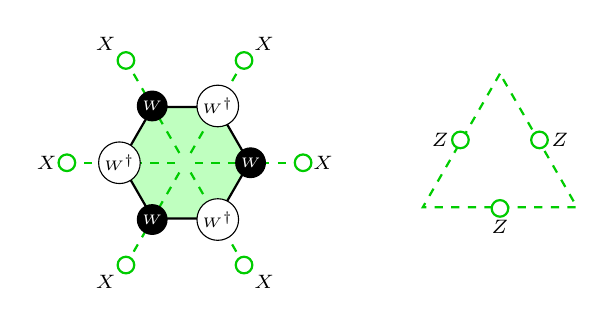
\begin{tikzpicture}
        \node[name = g2, regular polygon, regular polygon sides = 6, draw, inner sep = 0.5cm, fill=green, fill opacity=0.25, thick] at (0, 0) {};
        \node[name=g2a] at (g2.center) { };

        \foreach \n/\placement in {0/right, 1/above right, 2/above left, 3/left, 4/below left, 5/below right}
        {
        \draw[dashed, thick, green!80!black] (g2a) to (\n*60:1.5);
        \filldraw[shift=(g2.center), fill=white, draw = green!80!black, thick] (\n*60:1.5) circle (3pt) node[\placement] {\scriptsize\texttt{$X$}};
        }
        
        \foreach \anchor/\placement/\n/\fill/\text/\op in
        {corner 1/below/1/white/black/$W^\dagger$, corner 2/below/2/black/white/$W$, corner 3/right/3/white/black/$W^\dagger$, corner 4/above/4/black/white/$W$, corner 5/above/5/white/black/$W^\dagger$, corner 6/left/6/black/white/$W$}
        {
        \node[draw, circle, fill=\fill, inner sep = 1pt, text=\text] at (g2.\anchor) {\tiny{\op}};
        }



        \node[name=v, regular polygon, regular polygon sides = 3, draw =green!80!black, dashed, thick, inner sep = 0.4cm] at (4, 0) { };
        
        \filldraw[shift=(v.center), fill=white, draw = green!80!black, thick] (v.side 1) circle (3pt) node[left, inner sep = 4pt] {\scriptsize\texttt{$Z$}};
        \filldraw[shift=(v.center), fill=white, draw = green!80!black, thick] (v.side 2) circle (3pt) node[below, inner sep = 4pt] {\scriptsize\texttt{$Z$}};
        \filldraw[shift=(v.center), fill=white, draw = green!80!black, thick] (v.side 3) circle (3pt) node[right, inner sep = 4pt] {\scriptsize\texttt{$Z$}};
        
        
    \end{tikzpicture}
    }
\end{equation}
\begin{equation}
    \raisebox{-30pt}{
    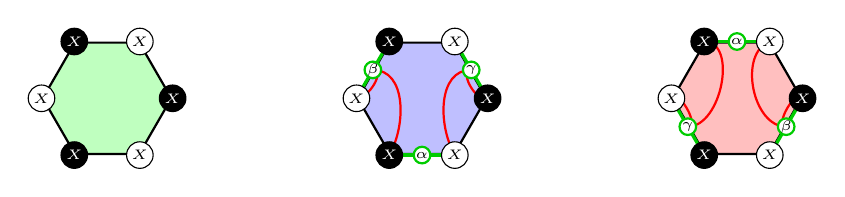
\begin{tikzpicture}
    
        \node[name= g, regular polygon, regular polygon sides = 6, draw, inner sep = 0.5cm, fill=green, fill opacity=0.25, thick] at (0, 0) { };

        \foreach \anchor/\placement/\n/\fill/\text/\op in
        {corner 1/below/1/white/black, corner 2/below/2/black/white, corner 3/right/3/white/black, corner 4/above/4/black/white, corner 5/above/5/white/black, corner 6/left/6/black/white}
        {
        \node[draw, circle, fill=\fill, inner sep = 1pt, text=\text] at (g.\anchor) {\tiny{$X$}};
        }


        \node[name= b5, regular polygon, regular polygon sides = 6, draw, inner sep = 0.5cm, fill=blue, fill opacity=0.25, thick] at (4, 0) {};

        \draw[-, red, thick] (b5.side 6) to[out=180, in=200] (b5.corner 6);
        \draw[-, red, thick] (b5.side 6) to[out=180, in=120] (b5.corner 5);

        \draw[-, red, thick] (b5.side 2) to[out=0, in=0] (b5.corner 3);
        \draw[-, red, thick] (b5.side 2) to[out=0, in=60] (b5.corner 4);
        
        \draw[-, green!80!black, very thick] (b5.corner 2) -- (b5.corner 3);
        \draw[-, green!80!black, very thick] (b5.corner 4) -- (b5.corner 5);
        \draw[-, green!80!black, very thick] (b5.corner 6) -- (b5.corner 1);

        \filldraw[fill=white, draw = green!80!black, thick] (b5.side 2) circle (3pt) node {\tiny{$\beta$}};
        \filldraw[fill=white, draw = green!80!black, thick] (b5.side 4) circle (3pt) node {\tiny{$\alpha$}};
        \filldraw[fill=white, draw = green!80!black, thick] (b5.side 6) circle (3pt) node {\tiny{$\gamma$}};

        \foreach \anchor/\placement/\n/\fill/\text/\op in
        {corner 1/below/1/white/black, corner 2/below/2/black/white, corner 3/right/3/white/black, corner 4/above/4/black/white, corner 5/above/5/white/black, corner 6/left/6/black/white}
        {
        \node[draw, circle, fill=\fill, inner sep = 1pt, text=\text] at (b5.\anchor) {\tiny{$X$}};
        }


        \node[name= r, regular polygon, regular polygon sides = 6, draw, inner sep = 0.5cm, fill=red, fill opacity=0.25, thick] at (8, 0) {};

        \draw[-, red, thick] (r.side 5) to[out=180, in=200] (r.corner 1);
        \draw[-, red, thick] (r.side 5) to[out=180, in=120] (r.corner 6);

        \draw[-, red, thick] (r.side 3) to[out=0, in=0] (r.corner 2);
        \draw[-, red, thick] (r.side 3) to[out=0, in=60] (r.corner 3);
        
        \draw[-, green!80!black, very thick] (r.corner 1) -- (r.corner 2);
        \draw[-, green!80!black, very thick] (r.corner 3) -- (r.corner 4);
        \draw[-, green!80!black, very thick] (r.corner 5) -- (r.corner 6);

        \filldraw[fill=white, draw = green!80!black, thick] (r.side 1) circle (3pt) node {\tiny{$\alpha$}};
        \filldraw[fill=white, draw = green!80!black, thick] (r.side 3) circle (3pt) node {\tiny{$\gamma$}};
        \filldraw[fill=white, draw = green!80!black, thick] (r.side 5) circle (3pt) node {\tiny{$\beta$}};

        \foreach \anchor/\placement/\n/\fill/\text/\op in
        {corner 1/below/1/white/black, corner 2/below/2/black/white, corner 3/right/3/white/black, corner 4/above/4/black/white, corner 5/above/5/white/black, corner 6/left/6/black/white}
        {
        \node[draw, circle, fill=\fill, inner sep = 1pt, text=\text] at (r.\anchor) {\tiny{$X$}};
        }
        
    \end{tikzpicture}
    }
\end{equation}
We have omitted the $Z$ hexagon stabilizers, which remain unchanged throughout the gauging procedure. 


\subsection{Gauging bivariate bicycle codes}
We now turn to some higher rate examples. In particular, we focus on the $[[144, 12, 12]]$ (Gross) code \cite{Bravyi2024faulttolerant}, which has received much attention recently, as it trades a modest amount of non-local connectivity for a large boost in encoding rate.

\subsubsection{Construction of self-dual bivariate bicycle codes}

In this example, we gauge a transversal symmetry on a \textit{self-dual bivariate bicycle} code with $k$ logical qubits. The transversal gate that we gauge is
\begin{equation}
    \T = \bar{W} = \prod_{A} W \prod_B \tilde{W}, \quad W = XS, \quad \tilde{W} = XS^\dagger
\end{equation} where, as with the color code, $A, B$ denote sublattices of a bipartite graph. 

Several papers have already considered self-dual versions of the bivariate bicycle code \cite{LiangChen2025Bivariate, Xu2025batched}.  We work with a different construction which is a generalization of the octagonal/square color code \cite{Bombin2006TopologicalQuantumDistillation}. The procedure we use to construct a self-dual code is generic and maps any initial CSS code to a new self-dual CSS code \cite{Criger2016NoiseThresholds422ToricCode, Bravyi2010MajoranaFermionCodes}; the action of $\bar{XS}$ on the new self-dual code is equivalent to the transversal $\CNOT$ between the original codeblocks (we work through the $\CNOT$ example below). 

Let the starting CSS code $C$ be an $[[n,k,d]]$ code with $X$ stabilizers $S_{X,1}, \cdots, S_{X, m_x}$ and $Z$ stabilizers $S_{Z,1}, \cdots, S_{Z, m_z}$.  Denote by $C_H$ the same code except with all stabilizers mapped to $S_{w,m_i} \rightarrow H^{\otimes n} S_{w,m_i} H^{\otimes n}$.  We also consider a subcode $C_{422}$ which is the self-dual $[[4,2,2]]$ code with stabilizers $X_1 X_2 X_3 X_4$ and $Z_1 Z_2 Z_3 Z_4$.  The logical operators of $C_{422}$ are $X_{L,1} = X_1 X_2$, $Z_{L,1} = Z_1 Z_3$, $X_{L,2} = X_1 X_3$, and $Z_{L,2} = Z_1 Z_2$.  

We form the self-dual code by pairing corresponding qubits on codeblocks $C$ and $C_H$, then encoding this pair of qubits into $C_{422}$, such that the first logical of $C_{422}$ corresponds to qubits of $C$, while the second logical corresponds to qubits of $C_H$. In other words, the new set of stabilizers contains
\begin{equation}
    \left \{ X_{j,1}X_{j,2}X_{j,3}X_{j,4}, ~~ Z_{j,1}Z_{j,2}Z_{j,3}Z_{j,4}\right \}_{j\in [n]}
\end{equation}
\begin{equation}
\begin{aligned}
    &\left \{\prod_{j\in \mathrm{supp}(S_{X,i})} X_{L,1,j} \right \}_i
    \quad \left \{\prod_{j\in \mathrm{supp}(S_{Z,i})} Z_{L,1,j}\right \}_i  \\
   &\left \{\prod_{j\in \mathrm{supp}(S_{X,i})} Z_{L,2,j}\right \}_i
   \quad \left \{\prod_{j\in \mathrm{supp}(S_{Z,i})} X_{L,2,j}\right \}_i 
\end{aligned}
\end{equation}
where $X_{L,1,j}$ corresponds to the first logical of the $[[4,2,2]]$ code that took the place of qubit $j$ in the original code (similarly for Z).  $X_{j,1}$ ($Z_{j,1}$) corresponds to the X (Z) operator on the first qubit in the $[[4,2,2]]$ code at location $j$.

We can quickly see that all of these stabilizers commute. The first and second group commute because the X and Z operators of the original code commute and this is preserved for the concatenated code since the two rows reference the same logical on the subcode (similarly for the third and fourth row).  The first and third group commute because they address different logicals in the subcode (same for second and fourth row).  The last row commutes with everything because the stabilizers of the subcode commute with logicals of the subcode.  The code is clearly self-dual because the first group is the Hadamard of the third (same for second and fourth) and the $[[4,2,2]]$ code is self-dual on its own.  

The code realized by this mapping takes an initial $[[n,k,d]]$ CSS code to a self-dual $[[4n, 2k, 2d]]$ CSS code.  The distance is doubled because each qubit in the support of an original logical is replaced by two qubits in the $[[4,2,2]]$ code.

If this construction is applied to the toric code, one generates the octagonal/square color code.  To realize a higher rate quantum LDPC code we choose to apply this general construction to the $[[144,12,12]]$ code of \cite{Bravyi2024faulttolerant} realizing a self-dual $[[576, 24, 24]]$ code. The stabilizers of the code are shown in Fig.~\ref{fig:bivariate_self_dual}: the code is CSS with two kinds of weight-12 checks, and one kind of weight-4 check. 

\begin{figure}[htbp]
    \centering
    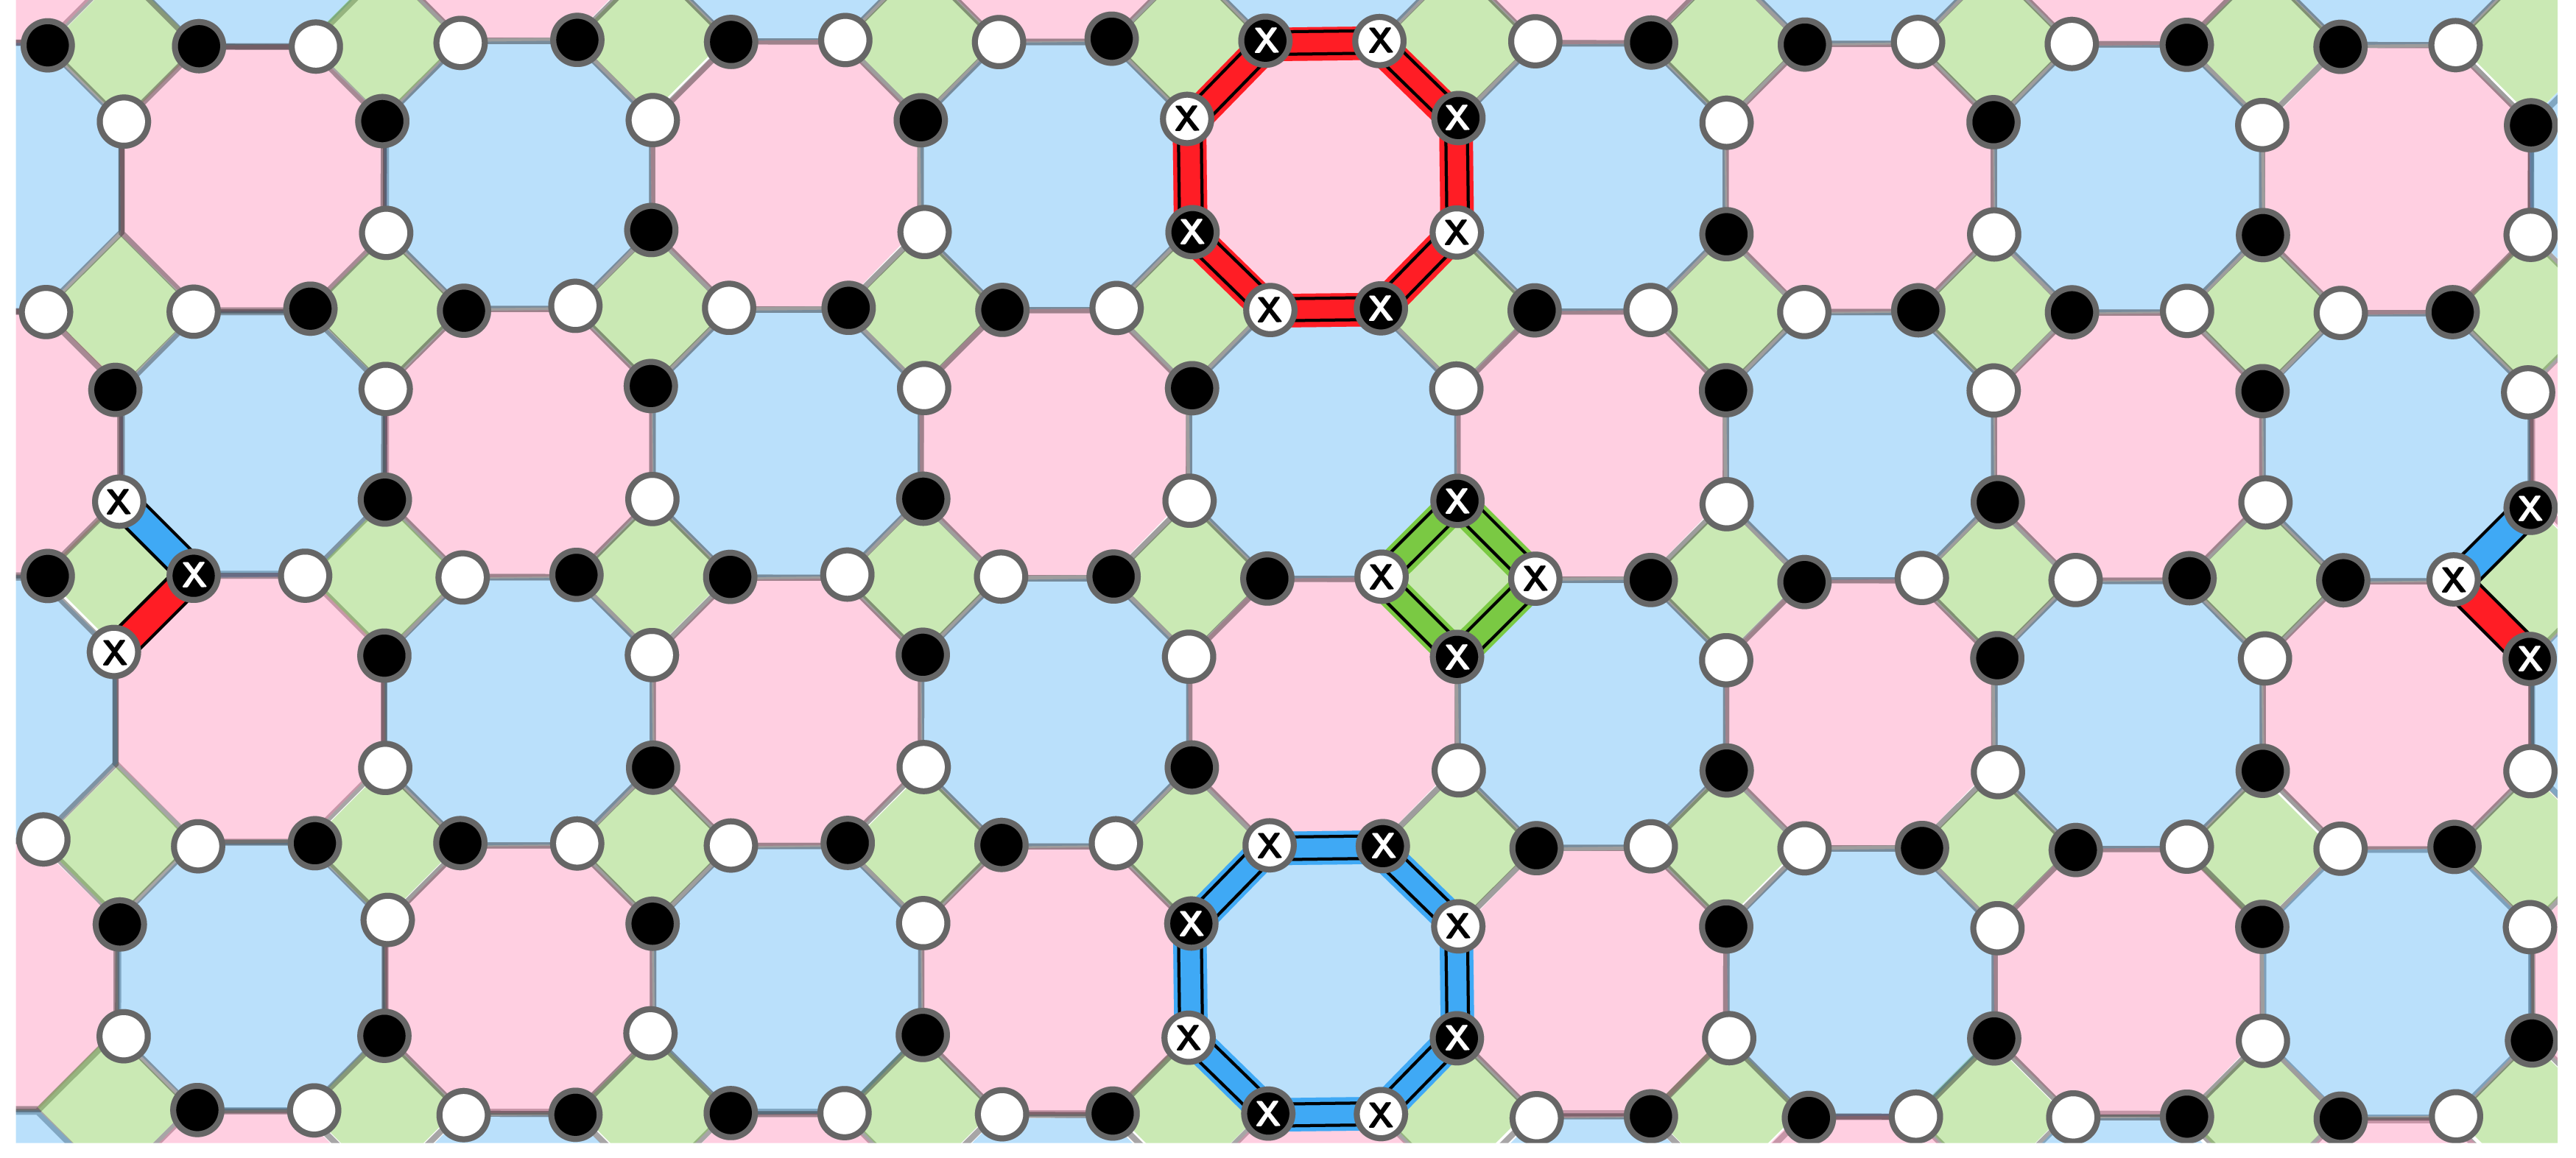
\includegraphics[width=0.7\linewidth]{figs/self-dual-bb.png}
    \caption{\textbf{Self-dual bivariate bicycle code}:  Lattice of the self-dual bivariate bicycle code, with the $A$ sublattice denoted by black circles, and the $B$ sublattice by white circles.  The red and blue highlights show the support of the stabilizers.  All stabilizers are present as both X and Z type. }
    \label{fig:bivariate_self_dual}
\end{figure}

Next we characterize the logical action of the transversal gate $\bar{W}$. The $X$ logicals of the self-dual code have a representative which is computed from the original $X$ logical $\bar{X}_L = \prod_{j\in \mathrm{supp}(\bar{X}_L)} X_j$ as $\bar{X}_{L,1} = \prod_{j\in \mathrm{supp}(\bar{X}_L)} X_{L,1,j}$ and $\bar{X}_{L,2} = \prod_{j\in \mathrm{supp}(\bar{Z}_L)} X_{L,2,j}$.  The same type of relation holds for the logical $Z$ operators.  As a consequence, the transversal $W$ has the following action:
\begin{align}
    \prod_{j=1}^n \CZ_{(L,1,j), (L,2,j)},
\quad \text{equivalent to}\quad
    \prod_{l=1}^k \CZ_{(\bar{1},l),(\bar{2},l)},
\end{align}
a product of logical $\CZ$ gates of the self-dual code. This set of logical $\CZ$ gates can be directly mapped back onto $C$ and $C_H$, as logicals $(\bar{1}, \cdot)$ correspond to logicals of $C$, and logicals $(\bar{2}, \cdot)$ correspond to $C_H$. As $C_H$ is related to $C$ by a Hadamard, the action is also equivalent to $\CNOT$ between two copies of $C$. 


\subsubsection{Gauging \texorpdfstring{$XS$}{XS} on a self-dual BB code} 
Below, we separate the $X$($Z$) stabilizers based on the color of the face on which they are supported:
\begin{equation}
    \green{S^{(g)}_{i, X(Z)}} \in \green{\mathcal{S}^{(g)}_{X(Z)}}, \quad \red{S^{(r)}_{i, X(Z)}} \in \red{\mathcal{S}^{(r)}_{X(Z)}}, \quad \blue{S^{(b)}_{i,X(Z)}}\in \blue{\mathcal{S}^{(b)}_{X(Z)}}
\end{equation}


Starting from the original code we apply the circuit-based gauging procedure.  As a first step we identify the vertex sets of the gauged code. Similar to the color code example above, we partition the qubits by green faces: i.e. the support of a $\green{S^{(g)}_{i, X}}$ stabilizer forms our vertex set. To begin the circuit-based gauging procedure we add a vertex ancilla $v$, initialized in the state $|+\rangle$, to each vertex set. We will denote this set of vertex ancillas by $V$. Since these vertex ancillas are in the state $|+\rangle$ they are stabilized by the single-qubit $X$ operator.  Hence the stabilizers at this point are those of the original code along with $\mathcal{S}_Q = \{X_i \mid i \in V\}$.   

Next we apply $CW$ (and $C\tilde{W}$) gates from each vertex ancilla $v \in V$ to the code qubits belonging to the corresponding vertex set.  Making use of the following relations
\begin{align}
    CW_{a\rightarrow b}\,X_b\,CW_{a\rightarrow b}^\dagger &= C(i Z)_{a\rightarrow b}\, X_b, \\
    C\tilde{W}_{a\rightarrow b}\,X_b\,C\tilde{W}_{a\rightarrow b}^\dagger &= C(-i Z)_{a\rightarrow b}\, X_b
\end{align}
we determine the stabilizers after the application of these gates.  The $Z$ stabilizers of the original code, $\green{\mathcal{S}^{(g)}_Z}, \red{\mathcal{S}^{(r)}_Z}, \blue{\mathcal{S}^{(b)}_Z}$, are unaffected by this circuit transformation.  A new set of stabilizers corresponding to each stabilizer in $\green{\mathcal{S}^{(g)}_X}$ is given by \begin{equation}
    \left \{\prod_{j \in \mathrm{supp}(\green{S^{(g)}_{X,i}})} X_j \, \CZ_{\vertexset{\green{S^{(g)}_{X,i}}}\rightarrow j} \mathrel{\bigg|} i \in V \right \}
\end{equation} where $\vertexset{\green{S^{(g)}_{X,i}}}$ returns the vertex ancilla qubit for a given green stabilizer.  We also add the stabilizers 
\begin{equation}
    \green{A_V'} = \left \{X_i \prod_{j \in \mathrm{supp}(\green{S^{(g)}_{X,i}}) \cap A} W_{j}  \prod_{k \in \mathrm{supp}(\green{S^{(g)}_{X,i}}) \cap B} \tilde{W}_{k} \mathrel{\bigg|} i \in V \right \}
\end{equation}
Here, $A$ is the sublattice where the transversal gate acts as $W$, while $B$ is the sublattice where it acts as $\tilde{W}$. Lastly we need to compute the updated $X$ stabilizers for the octagonal (red, blue) stabilizers.  These are described by 
\begin{equation}
    \left \{ \prod_{j \in \mathrm{supp}(\red{S^{(r)}_{X,i}})} X_j \CZ_{\Sigma^{-1}(j)\rightarrow j} \right \}, \quad \left \{ \prod_{j \in \mathrm{supp}(\blue{S^{(b)}_{X,i}})} X_j \CZ_{\Sigma^{-1}(j)\rightarrow j} \right \}
\end{equation}
In other words, we dress the $X$ stabilizers with $\CZ$ gates supported on each qubit and its corresponding vertex ancilla.  

Next we add gauge qubits into the system on the outgoing edges from the vertex sets.  The choice of edges here is up to the convention and ours is shown in Fig.~\ref{fig:gauged_bivariate_self_dual}; we have set the gauging graph to be the square sublattice naturally formed by the green faces with additional long range edges set by the connectivity of the octagonal stabilizers. Let the set of gauge qubits be $G$ and $\partial$ the mapping from gauge qubits to the neighboring vertex ancillas in $V$. The gauge qubits are initialized in the state $|0\rangle$. We entangle all of the gauge qubits with the neighboring vertex ancillas using the CSS cluster entangler. In addition to adding the cluster state edge stabilizers given by 
\begin{equation}
    \left \{Z_i \prod_{j\in \delta(i)} Z_{j}\mid i \in G \right \},
\end{equation}
the $\green{A_V'}$ are modified to the form 
\begin{equation}
    \green{A_V''} = \left \{X_i \prod_{\ell \mid i \in \delta(\ell)} X_{\ell} \prod_{j \in \mathrm{supp}(\green{S^{(g)}_{X,i}}) \cap A} W_{j}  \prod_{k \in \mathrm{supp}(\green{S^{(g)}_{X,i}}) \cap B} \tilde{W}_{k} \mathrel{\bigg|} i \in V \right \}
\end{equation}
The other stabilizers are untouched by the cluster state entangler. The stabilizers at this point are shown in Fig.~\ref{fig:gauged_bivariate_self_dual}a, with the omission of the $S_Z$ stabilizers which have not changed.   

The last step of constructing the gauged code is to measure all of the vertex ancillas in the $X$ basis.  We aim to find new stabilizers which commute with this measurement operation (perhaps up to other stabilizers). The initial $Z$ stabilizers of the code trivially commute with this measurement, as they were untouched by the gauging circuit. The $A_V''$ simply have their $X$ support on the vertex ancilla removed: 
\begin{equation}
    \green{A_V''} \to \green{\av} = \left \{ \prod_{\ell \mid i \in \delta(\ell)} X_{\ell} \prod_{j \in \mathrm{supp}(\green{S^{(g)}_{X,i}}) \cap A} W_{j}  \prod_{k \in \mathrm{supp}(\green{S^{(g)}_{X,i}}) \cap B} \tilde{W}_{k} \mathrel{\bigg|} i \in V \right \}
\end{equation}
Additionally we have loop stabilizers formed from products of the edge stabilizers around every cycle of the gauging graph: 
\begin{equation}
    \bp = \prod_{i \mid \partial(i) = 0} Z_i
\end{equation}
To determine the final form of the other stabilizers, we will again take advantage of Eq.~\ref{eq:CZ-deformation}. We can pull a controlled-$\green{S^{(g)}_{Z, i}}$ stabilizer out of each $\green{S^{(g)}_{X, i}}$: 
\begin{equation}
\begin{aligned}
    \left \{\prod_{j \in \mathrm{supp}(\green{S^{(g)}_{X,i}})} X_j \, \CZ_{\vertexset{\green{S^{(g)}_{X,i}}}\rightarrow j} \mathrel{\bigg|} i \in V \right \} &\rightarrow \left \{\prod_{j \in \mathrm{supp}(\green{S^{(g)}_{X,i}})} X_j \, \mathsf{C}_i\green{S^{(g)}_{Z, i}}\mathrel{\bigg|} i \in V \right \}\\
    &\xrightarrow{\green{S^{(g)}_{Z, i}} = +1} \left \{\prod_{j \in \mathrm{supp}(\green{S^{(g)}_{X,i}})} X_j \mathrel{\bigg|} i \in V \right \}
\end{aligned}
\end{equation}
Similarly, we can pull a controlled-$\red{S^{(r)}_{Z, i}} (\blue{S^{(b)}_{Z, i}})$ out of the deformed $\red{S^{(r)}_{X, i}} (\blue{S^{(b)}_{X, i}})$. However, since these stabilizers are supported between multiple vertex sets, when we pull out the controlled-stabilizers, we will leave behind some $\CZ$ gates between the original qubits and the edge ancilla. 

The final set of gauged stabilizers are pictured in Fig.~\ref{fig:gauged_bivariate_self_dual}b). 




\begin{figure}[htbp]
    \centering
    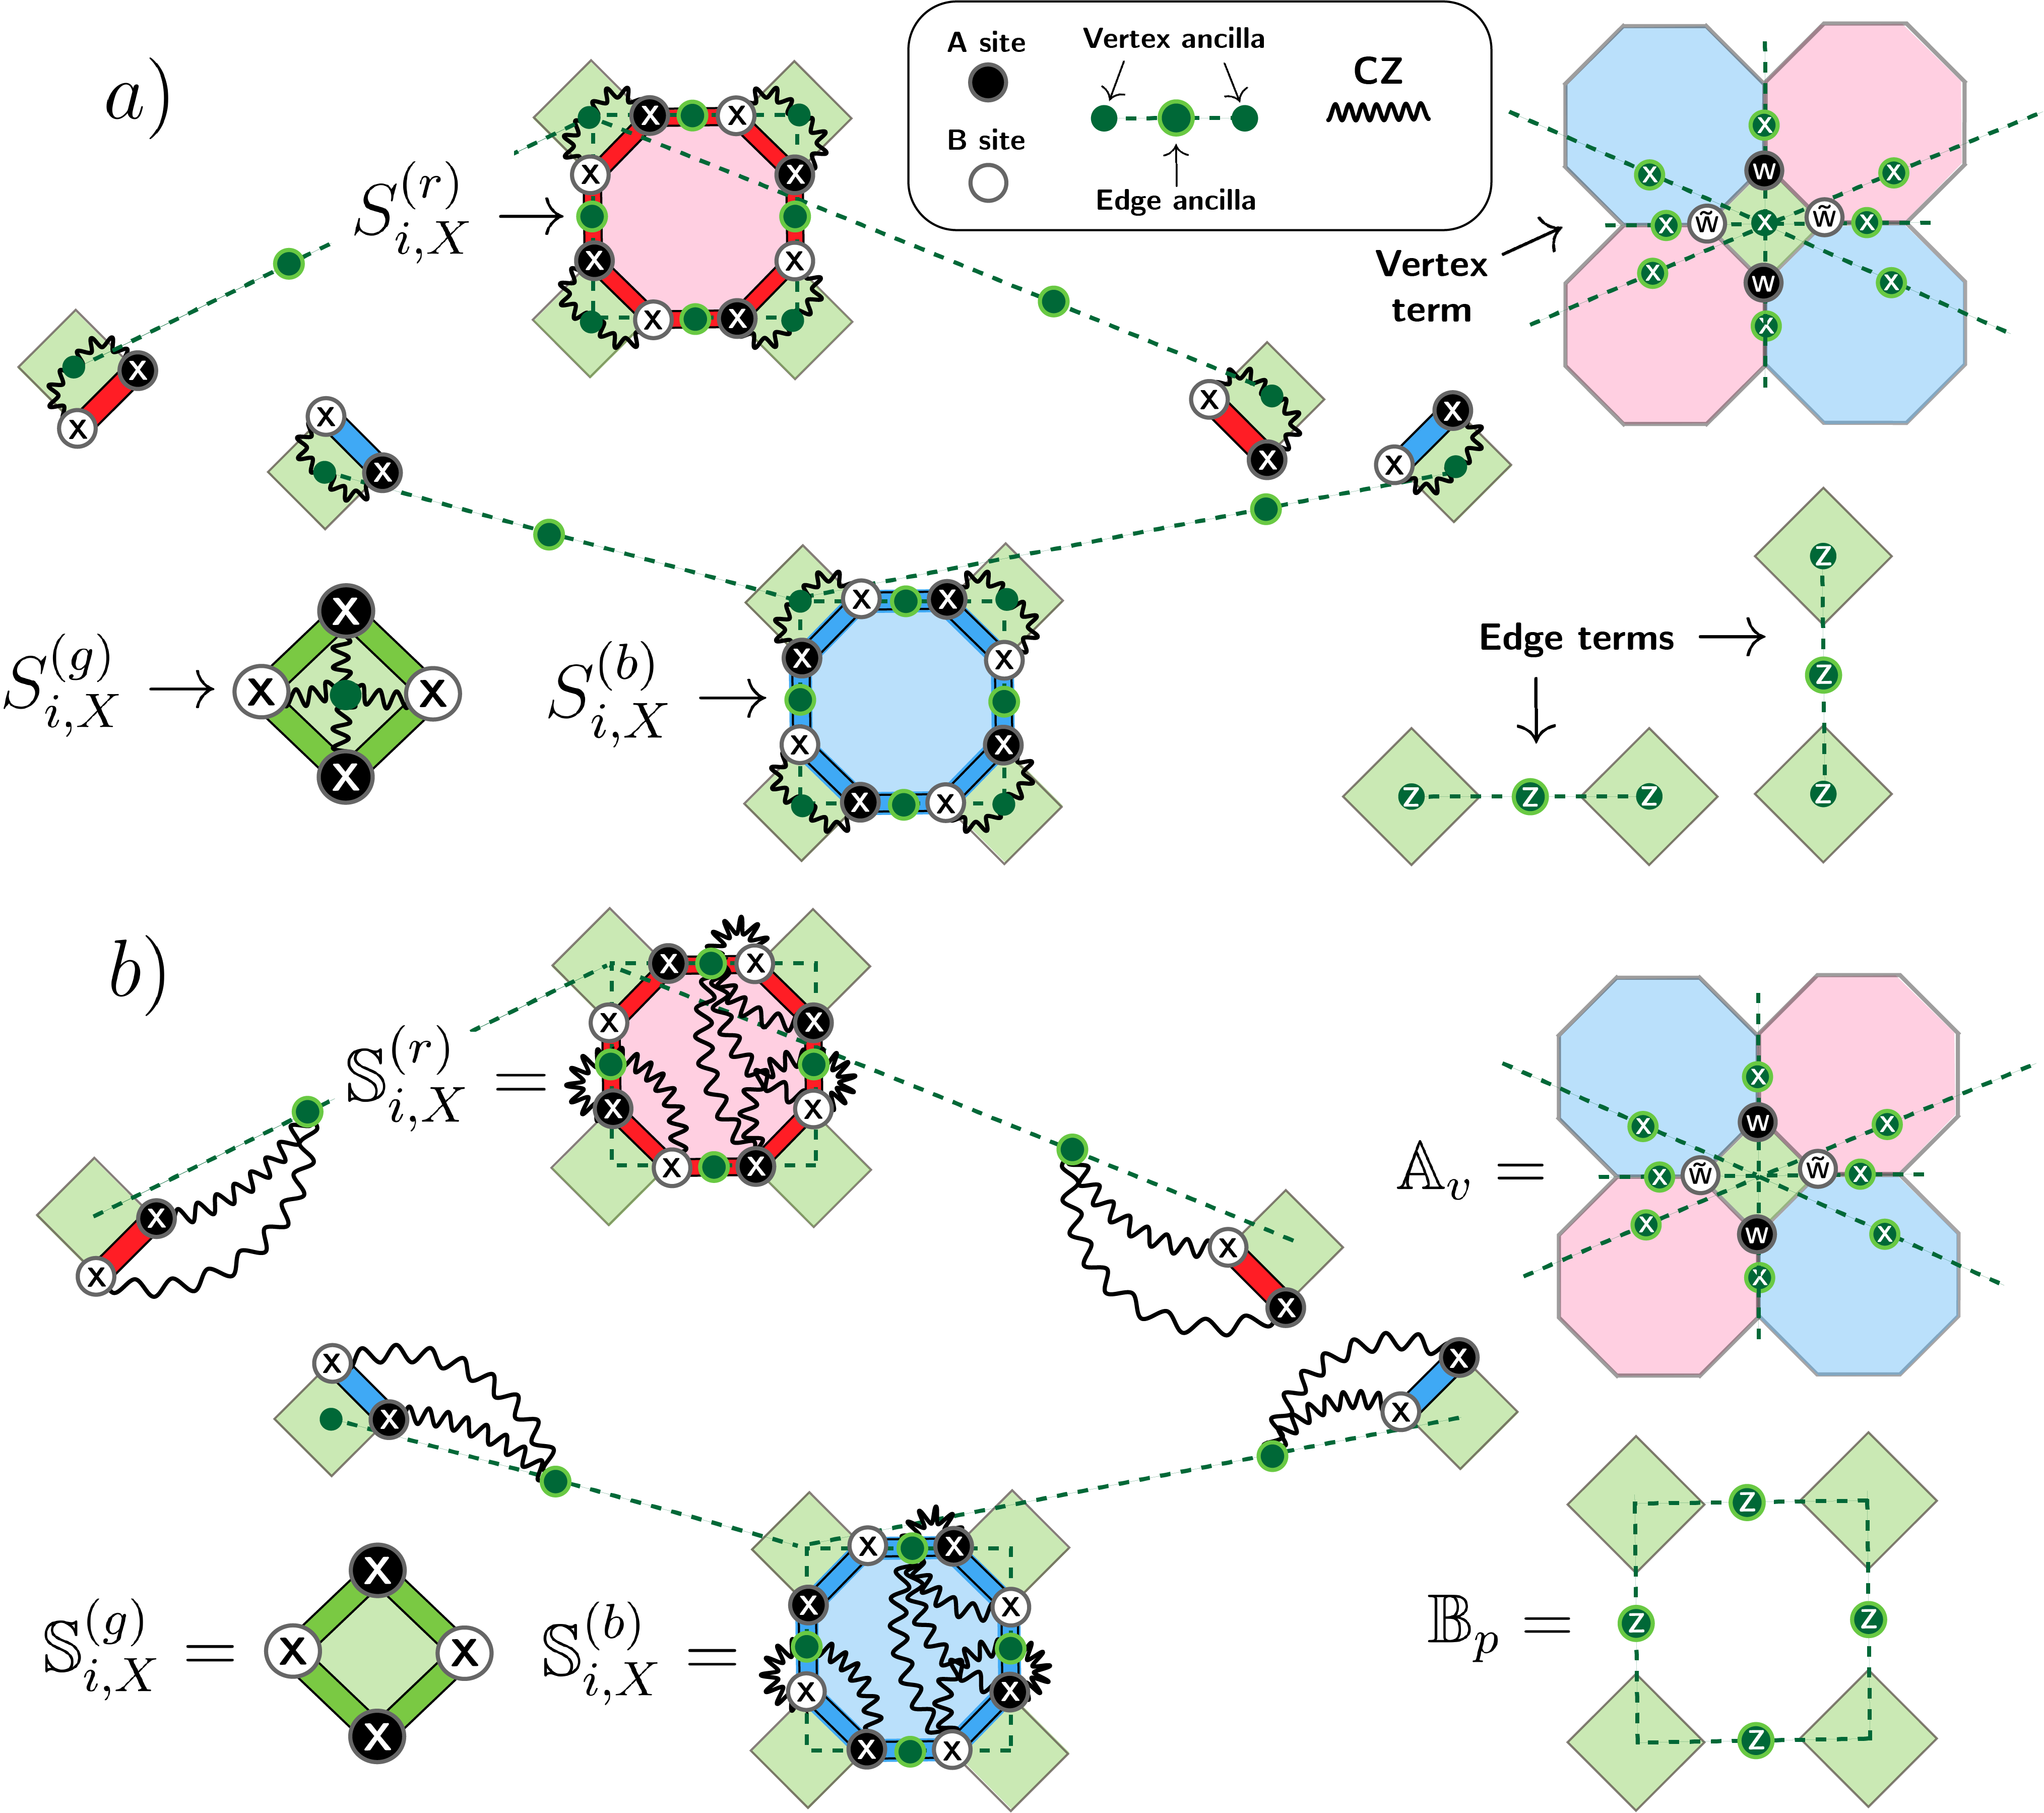
\includegraphics[width=0.9\linewidth]{figs/bb-xs-stabilizers.png}
    \caption{\textbf{Gauged self-dual bivariate bicycle code}:  We show selected stabilizers at different stages of the gauging procedure. Physical qubits are placed at the vertices of the underlying 4.8.8 tiling. (a) Intermediate step where we have added vertex ancillas, performed the entangling gates between vertex ancillas and neighboring qubits, added new edges and gauge qubits, and performed the cluster state entangler. (b) Final gauged code. Squigly lines represent $\CZ$ gates that result from dressing.  }
    \label{fig:gauged_bivariate_self_dual}
\end{figure}

As an aside, we note that gauging the $XS$ symmetry of the color code yields a topological code with the same properties as the quantum double of $D_4$. This is a consequence of the fact $D_4 = \mathbb{Z}_2 \times \mathbb{Z}_2 \rtimes \mathbb{Z}_2$ .\footnote{Usually, we write $D_4 = \mathbb{Z}_4 \rtimes \mathbb{Z}_2$, but it can equivalently be expressed as $\mathbb{Z}_2 \times \mathbb{Z}_2 \rtimes \mathbb{Z}_2$, as both $\mathbb{Z}_4$ and $\mathbb{Z}_2 \times \mathbb{Z}_2$ are normal subgroups.} In essence, when we gauge, we implement this semi-direct product \cite{Tantivasadakarn_2023}. The color code is equivalent to two copies of the $\mathbb{Z}_2$ quantum double, more commonly known as the toric code--- gauging a layer-swap $\mathbb{Z}_2$ symmetry on this model leads to a $D_4$ anyon model. 

Recent work~\cite{LiangChen2025Bivariate} has shown that placing the stabilizers of the $\llbracket 144, 12, 12\rrbracket$ code on an infinite square lattice yields a code equivalent to 8 copies of the toric code. As we used two copies of the input BB code, we should expect the self-dual code considered here to be equivalent to 16 copies of the toric code. Thus, we can conjecture that the $XS$-gauged model has topological order described by $\mathbb{Z}_2^{16} \rtimes \mathbb{Z}_2$.

\subsubsection{Gauging \texorpdfstring{$\CNOT$}{CNOT} on bivariate bicycle codes}
Here we gauge the transversal $\CNOT$ between a pair of bivariate bicycle codes\footnote{We note that this example was also discussed in Ref.~\cite{christos2026nonabelianquantumlowdensityparity}.}. The bivariate bicycle code is a CSS code and hence admits a transversal $\CNOT$ gate.  By gauging the transversal $\CNOT$ symmetry we are measuring the operator $\CNOT^{\otimes n}$; this does not allow us to individually resolve the value of the $\CNOT$ measurement for each logical qubit--- this is not an addressable measurement.

We pick vertex sets consisting of pairs of corresponding qubits in the two codeblocks; the gauging operation is shown step-by-step in Fig.~\ref{fig:bb_cnot_gauging}, with Fig.~\ref{fig:bb_cnot_gauging}e) depicting the stabilizers of the gauged code.

\begin{figure}[htbp]
    \centering
    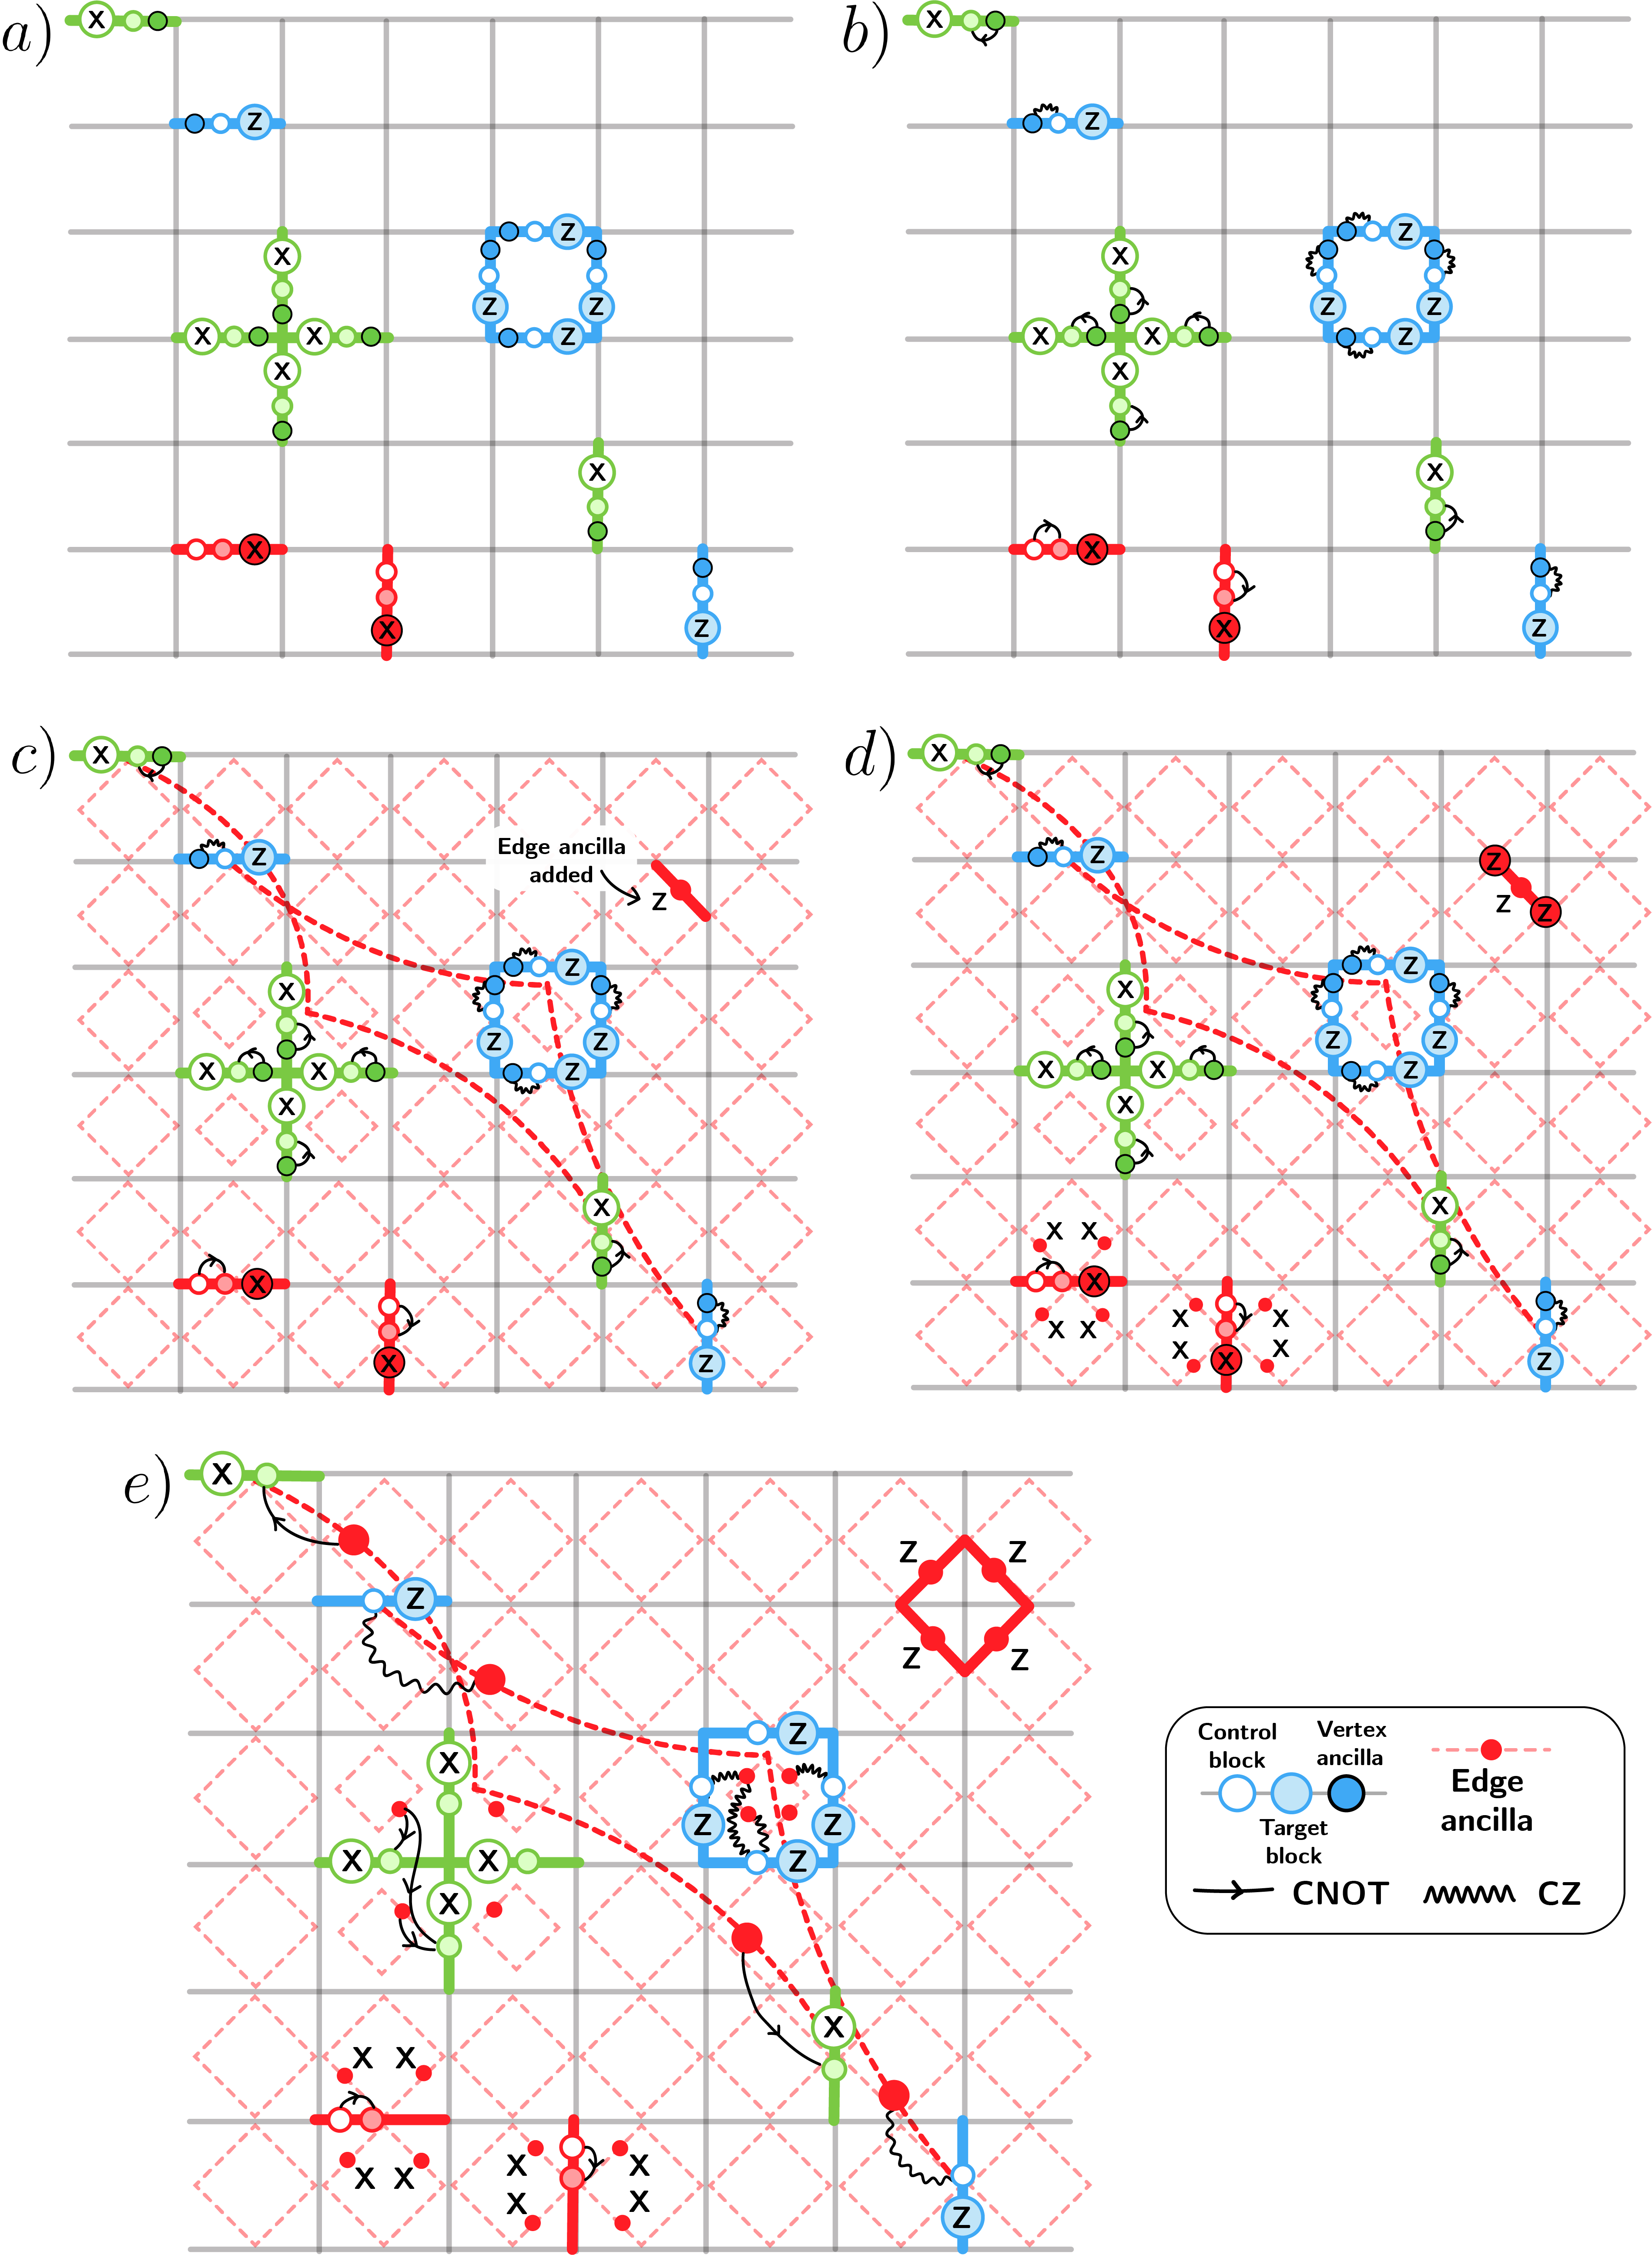
\includegraphics[width=0.75\linewidth]{figs/examples/bb-cnot-example.png}
    \caption{\textbf{Gauging $\CNOT$ between bivariate bicycle codes: } We show all the steps for gauging a $\CNOT$ between two bivariate bicycle codes.  In this example a gauging vertex is associated to each pair of qubits in the support of a $\CNOT$. (a) We show control-block $X$ stabilizers (green), target-block $Z$ stabilizers (blue), and vertex ancilla (red). (b) Stabilizers after performing the $CCNOT$ operation between vertex ancillas and the qubits in both codeblocks. (c) The gauging graph is pictured in red dashed lines (only some of the long-range connections are pictured and the lattice is slightly deformed around the support of the stabilizers purely for visual clarity), edge ancillas initialized in $\ket{0}$. (d) Stabilizers after the cluster state entangler. (e) Final stabilizers after projecting vertex ancilla onto $\ket{+}$.}
    \label{fig:bb_cnot_gauging}
\end{figure}


\subsection{Gauging qudit symmetries}
Here, to exemplify the general gauging procedure, we consider examples of  non-$\mathbb{Z}_2$ Clifford symmetries on qubit and qudit codes. 

\subsubsection{Gauging \texorpdfstring{$HS$}{HS} on color codes and BB codes}
The color code, being self-dual, possesses a transversal facet gate $HS$. This is an order 3 permutation that takes $X \to Y \to Z$. As with the $XS$ gate, the physical representation of the logical facet gate $F = HS$ has different action on the $A$ and $B$ sublattices: $\T = \prod_{A} F \prod_B \tilde{F}$, where $\tilde{F} = HS^\dagger$. The facet gate is a $\mathbb{Z}_3$ symmetry: $(HS)^3 = (HS^\dagger)^3 = \id$. Thus, we use \emph{qutrit} ancillas to perform the gauging. We write qutrit operators as $\mathcal{X}, \mathcal{Z}$: $\mathcal{Z}\mathcal{X} = e^{2\pi i /3} \mathcal{XZ}$. As we are gauging a $\mathbb{Z}_3$ symmetry on top of a code with associated group $\mathbb{Z}_2 \times \mathbb{Z}_2$ (being related to two copies of the $\mathbb{Z}_2$ toric code), we should expect the resulting model to be described by $(\mathbb{Z}_2 \times \mathbb{Z}_2) \rtimes \mathbb{Z}_3 \cong A_4$.

We make the same choice of vertex set as the prior example: each green hexagon. The control gate we use for the gauging is a mixed qutrit-qubit gate, with the qutrit acting as the control and the qubit as the target:
\begin{equation}
    \mathcal{C}_i F_j = \sum_{a = 0}^2 \dyad{a}_i \otimes F^a_j
\end{equation}

After gauging, we find the following checks:
\begin{equation}
    \raisebox{-50pt}{
    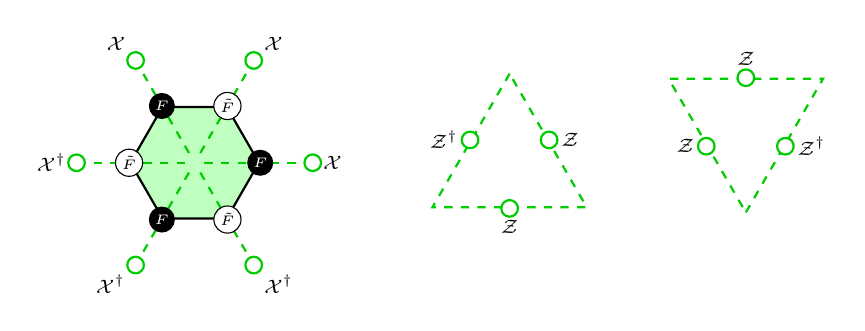
\begin{tikzpicture}
        \node[name = g2, regular polygon, regular polygon sides = 6, draw, inner sep = 0.5cm, fill=green, fill opacity=0.25, thick] at (0, 0) {};
        \node[name=g2a] at (g2.center) { };

        \foreach \n/\placement in {0/right, 1/above right, 2/above left}
        {
        \draw[dashed, thick, green!80!black] (g2a) to (\n*60:1.5);
        \filldraw[shift=(g2.center), fill=white, draw = green!80!black, thick] (\n*60:1.5) circle (3pt) node[\placement] {\scriptsize\texttt{$\mathcal{X}$}};
        }

        \foreach \n/\placement in {3/left, 4/below left, 5/below right}
        {
        \draw[dashed, thick, green!80!black] (g2a) to (\n*60:1.5);
        \filldraw[shift=(g2.center), fill=white, draw = green!80!black, thick] (\n*60:1.5) circle (3pt) node[\placement] {\scriptsize\texttt{$\mathcal{X}^\dagger$}};
        }
        
        \foreach \anchor/\placement/\n/\fill/\text/\op in
        {corner 1/below/1/white/black/$\tilde{F}$, corner 2/below/2/black/white/$F$, corner 3/right/3/white/black/$\tilde{F}$, corner 4/above/4/black/white/$F$, corner 5/above/5/white/black/$\tilde{F}$, corner 6/left/6/black/white/$F$}
        {
        \node[draw, circle, fill=\fill, inner sep = 1pt, text=\text] at (g2.\anchor) {\tiny{\op}};
        }



        \node[name=v, regular polygon, regular polygon sides = 3, draw =green!80!black, dashed, thick, inner sep = 0.4cm] at (4, 0) { };
        
        \filldraw[shift=(v.center), fill=white, draw = green!80!black, thick] (v.side 1) circle (3pt) node[left, inner sep = 4pt] {\scriptsize\texttt{$\mathcal{Z}^\dagger$}};
        \filldraw[shift=(v.center), fill=white, draw = green!80!black, thick] (v.side 2) circle (3pt) node[below, inner sep = 4pt] {\scriptsize\texttt{$\mathcal{Z}$}};
        \filldraw[shift=(v.center), fill=white, draw = green!80!black, thick] (v.side 3) circle (3pt) node[right, inner sep = 4pt] {\scriptsize\texttt{$\mathcal{Z}$}};


        \node[name=v, regular polygon, regular polygon sides = 3, draw =green!80!black, dashed, thick, inner sep = 0.4cm, rotate=180] at (7, 0.5) { };
        
        \filldraw[shift=(v.center), fill=white, draw = green!80!black, thick] (v.side 1) circle (3pt) node[right, inner sep = 4pt] {\scriptsize\texttt{$\mathcal{Z}^\dagger$}};
        \filldraw[shift=(v.center), fill=white, draw = green!80!black, thick] (v.side 2) circle (3pt) node[above, inner sep = 4pt] {\scriptsize\texttt{$\mathcal{Z}$}};
        \filldraw[shift=(v.center), fill=white, draw = green!80!black, thick] (v.side 3) circle (3pt) node[left, inner sep = 4pt] {\scriptsize\texttt{$\mathcal{Z}$}};
        
        
    \end{tikzpicture}
    }
\end{equation}
\begin{equation}
    \raisebox{-30pt}{
    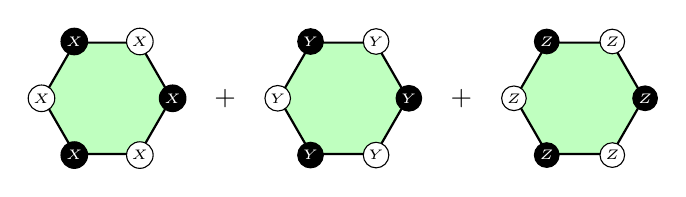
\begin{tikzpicture}
        \node[name= g, regular polygon, regular polygon sides = 6, draw, inner sep = 0.5cm, fill=green, fill opacity=0.25, thick] at (0, 0) { };

        \foreach \anchor/\placement/\n/\fill/\text/\op in
        {corner 1/below/1/white/black, corner 2/below/2/black/white, corner 3/right/3/white/black, corner 4/above/4/black/white, corner 5/above/5/white/black, corner 6/left/6/black/white}
        {
        \node[draw, circle, fill=\fill, inner sep = 1pt, text=\text] at (g.\anchor) {\tiny{$X$}};
        }

        \node at (1.5, 0) {$+$};

        \node[name= g, regular polygon, regular polygon sides = 6, draw, inner sep = 0.5cm, fill=green, fill opacity=0.25, thick] at (3, 0) { };

        \foreach \anchor/\placement/\n/\fill/\text/\op in
        {corner 1/below/1/white/black, corner 2/below/2/black/white, corner 3/right/3/white/black, corner 4/above/4/black/white, corner 5/above/5/white/black, corner 6/left/6/black/white}
        {
        \node[draw, circle, fill=\fill, inner sep = 1pt, text=\text] at (g.\anchor) {\tiny{$Y$}};
        }

        \node at (4.5, 0) {$+$};

        \node[name= g, regular polygon, regular polygon sides = 6, draw, inner sep = 0.5cm, fill=green, fill opacity=0.25, thick] at (6, 0) { };

        \foreach \anchor/\placement/\n/\fill/\text/\op in
        {corner 1/below/1/white/black, corner 2/below/2/black/white, corner 3/right/3/white/black, corner 4/above/4/black/white, corner 5/above/5/white/black, corner 6/left/6/black/white}
        {
        \node[draw, circle, fill=\fill, inner sep = 1pt, text=\text] at (g.\anchor) {\tiny{$Z$}};
        }
    \end{tikzpicture}
    }
\end{equation}
\begin{equation}
    \raisebox{-30pt}{
    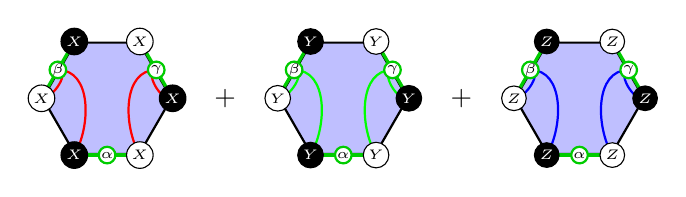
\begin{tikzpicture}
        
        \node[name= b5, regular polygon, regular polygon sides = 6, draw, inner sep = 0.5cm, fill=blue, fill opacity=0.25, thick] at (0, 0) {};

        \draw[-, red, thick] (b5.side 6) to[out=180, in=200] (b5.corner 6);
        \draw[-, red, thick] (b5.side 6) to[out=180, in=120] (b5.corner 5);

        \draw[-, red, thick] (b5.side 2) to[out=0, in=0] (b5.corner 3);
        \draw[-, red, thick] (b5.side 2) to[out=0, in=60] (b5.corner 4);
        
        \draw[-, green!80!black, very thick] (b5.corner 2) -- (b5.corner 3);
        \draw[-, green!80!black, very thick] (b5.corner 4) -- (b5.corner 5);
        \draw[-, green!80!black, very thick] (b5.corner 6) -- (b5.corner 1);

        \filldraw[fill=white, draw = green!80!black, thick] (b5.side 2) circle (3pt) node {\tiny{$\beta$}};
        \filldraw[fill=white, draw = green!80!black, thick] (b5.side 4) circle (3pt) node {\tiny{$\alpha$}};
        \filldraw[fill=white, draw = green!80!black, thick] (b5.side 6) circle (3pt) node {\tiny{$\gamma$}};

        \foreach \anchor/\placement/\n/\fill/\text/\op in
        {corner 1/below/1/white/black, corner 2/below/2/black/white, corner 3/right/3/white/black, corner 4/above/4/black/white, corner 5/above/5/white/black, corner 6/left/6/black/white}
        {
        \node[draw, circle, fill=\fill, inner sep = 1pt, text=\text] at (b5.\anchor) {\tiny{$X$}};
        }

        \node at (1.5, 0) {$+$};
        
        
        \node[name= b5, regular polygon, regular polygon sides = 6, draw, inner sep = 0.5cm, fill=blue, fill opacity=0.25, thick] at (3, 0) {};

        \draw[-, green, thick] (b5.side 6) to[out=180, in=200] (b5.corner 6);
        \draw[-, green, thick] (b5.side 6) to[out=180, in=120] (b5.corner 5);

        \draw[-, green, thick] (b5.side 2) to[out=0, in=0] (b5.corner 3);
        \draw[-, green, thick] (b5.side 2) to[out=0, in=60] (b5.corner 4);
        
        \draw[-, green!80!black, very thick] (b5.corner 2) -- (b5.corner 3);
        \draw[-, green!80!black, very thick] (b5.corner 4) -- (b5.corner 5);
        \draw[-, green!80!black, very thick] (b5.corner 6) -- (b5.corner 1);

        \filldraw[fill=white, draw = green!80!black, thick] (b5.side 2) circle (3pt) node {\tiny{$\beta$}};
        \filldraw[fill=white, draw = green!80!black, thick] (b5.side 4) circle (3pt) node {\tiny{$\alpha$}};
        \filldraw[fill=white, draw = green!80!black, thick] (b5.side 6) circle (3pt) node {\tiny{$\gamma$}};

        \foreach \anchor/\placement/\n/\fill/\text/\op in
        {corner 1/below/1/white/black, corner 2/below/2/black/white, corner 3/right/3/white/black, corner 4/above/4/black/white, corner 5/above/5/white/black, corner 6/left/6/black/white}
        {
        \node[draw, circle, fill=\fill, inner sep = 1pt, text=\text] at (b5.\anchor) {\tiny{$Y$}};
        }

        \node at (4.5, 0) {$+$};


        \node[name= b5, regular polygon, regular polygon sides = 6, draw, inner sep = 0.5cm, fill=blue, fill opacity=0.25, thick] at (6, 0) {};

        \draw[-, blue, thick] (b5.side 6) to[out=180, in=200] (b5.corner 6);
        \draw[-, blue, thick] (b5.side 6) to[out=180, in=120] (b5.corner 5);

        \draw[-, blue, thick] (b5.side 2) to[out=0, in=0] (b5.corner 3);
        \draw[-, blue, thick] (b5.side 2) to[out=0, in=60] (b5.corner 4);
        
        \draw[-, green!80!black, very thick] (b5.corner 2) -- (b5.corner 3);
        \draw[-, green!80!black, very thick] (b5.corner 4) -- (b5.corner 5);
        \draw[-, green!80!black, very thick] (b5.corner 6) -- (b5.corner 1);

        \filldraw[fill=white, draw = green!80!black, thick] (b5.side 2) circle (3pt) node {\tiny{$\beta$}};
        \filldraw[fill=white, draw = green!80!black, thick] (b5.side 4) circle (3pt) node {\tiny{$\alpha$}};
        \filldraw[fill=white, draw = green!80!black, thick] (b5.side 6) circle (3pt) node {\tiny{$\gamma$}};

        \foreach \anchor/\placement/\n/\fill/\text/\op in
        {corner 1/below/1/white/black, corner 2/below/2/black/white, corner 3/right/3/white/black, corner 4/above/4/black/white, corner 5/above/5/white/black, corner 6/left/6/black/white}
        {
        \node[draw, circle, fill=\fill, inner sep = 1pt, text=\text] at (b5.\anchor) {\tiny{$Z$}};
        }

        
    \end{tikzpicture}
    }
\end{equation}
\begin{equation}
    \raisebox{-30pt}{
    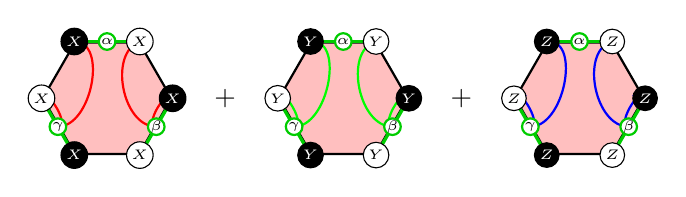
\begin{tikzpicture}


        \node[name= r, regular polygon, regular polygon sides = 6, draw, inner sep = 0.5cm, fill=red, fill opacity=0.25, thick] at (0, 0) {};

        \draw[-, red, thick] (r.side 5) to[out=180, in=200] (r.corner 1);
        \draw[-, red, thick] (r.side 5) to[out=180, in=120] (r.corner 6);

        \draw[-, red, thick] (r.side 3) to[out=0, in=0] (r.corner 2);
        \draw[-, red, thick] (r.side 3) to[out=0, in=60] (r.corner 3);
        
        \draw[-, green!80!black, very thick] (r.corner 1) -- (r.corner 2);
        \draw[-, green!80!black, very thick] (r.corner 3) -- (r.corner 4);
        \draw[-, green!80!black, very thick] (r.corner 5) -- (r.corner 6);

        \filldraw[fill=white, draw = green!80!black, thick] (r.side 1) circle (3pt) node {\tiny{$\alpha$}};
        \filldraw[fill=white, draw = green!80!black, thick] (r.side 3) circle (3pt) node {\tiny{$\gamma$}};
        \filldraw[fill=white, draw = green!80!black, thick] (r.side 5) circle (3pt) node {\tiny{$\beta$}};

        \foreach \anchor/\placement/\n/\fill/\text/\op in
        {corner 1/below/1/white/black, corner 2/below/2/black/white, corner 3/right/3/white/black, corner 4/above/4/black/white, corner 5/above/5/white/black, corner 6/left/6/black/white}
        {
        \node[draw, circle, fill=\fill, inner sep = 1pt, text=\text] at (r.\anchor) {\tiny{$X$}};
        }

        \node at (1.5, 0) {$+$};


        \node[name= r, regular polygon, regular polygon sides = 6, draw, inner sep = 0.5cm, fill=red, fill opacity=0.25, thick] at (3, 0) {};

        \draw[->, green, thick] (r.side 5) to[out=180, in=200] (r.corner 1);
        \draw[->, green, thick] (r.side 5) to[out=180, in=120] (r.corner 6);

        \draw[->, green, thick] (r.side 3) to[out=0, in=0] (r.corner 2);
        \draw[->, green, thick] (r.side 3) to[out=0, in=60] (r.corner 3);
        
        \draw[-, green!80!black, very thick] (r.corner 1) -- (r.corner 2);
        \draw[-, green!80!black, very thick] (r.corner 3) -- (r.corner 4);
        \draw[-, green!80!black, very thick] (r.corner 5) -- (r.corner 6);

        \filldraw[fill=white, draw = green!80!black, thick] (r.side 1) circle (3pt) node {\tiny{$\alpha$}};
        \filldraw[fill=white, draw = green!80!black, thick] (r.side 3) circle (3pt) node {\tiny{$\gamma$}};
        \filldraw[fill=white, draw = green!80!black, thick] (r.side 5) circle (3pt) node {\tiny{$\beta$}};

        \foreach \anchor/\placement/\n/\fill/\text/\op in
        {corner 1/below/1/white/black, corner 2/below/2/black/white, corner 3/right/3/white/black, corner 4/above/4/black/white, corner 5/above/5/white/black, corner 6/left/6/black/white}
        {
        \node[draw, circle, fill=\fill, inner sep = 1pt, text=\text] at (r.\anchor) {\tiny{$Y$}};
        }


        \node[name= r, regular polygon, regular polygon sides = 6, draw, inner sep = 0.5cm, fill=red, fill opacity=0.25, thick] at (6, 0) {};

        \draw[->, blue, thick] (r.side 5) to[out=180, in=200] (r.corner 1);
        \draw[->, blue, thick] (r.side 5) to[out=180, in=120] (r.corner 6);

        \draw[->, blue, thick] (r.side 3) to[out=0, in=0] (r.corner 2);
        \draw[->, blue, thick] (r.side 3) to[out=0, in=60] (r.corner 3);
        
        \draw[-, green!80!black, very thick] (r.corner 1) -- (r.corner 2);
        \draw[-, green!80!black, very thick] (r.corner 3) -- (r.corner 4);
        \draw[-, green!80!black, very thick] (r.corner 5) -- (r.corner 6);

        \filldraw[fill=white, draw = green!80!black, thick] (r.side 1) circle (3pt) node {\tiny{$\alpha$}};
        \filldraw[fill=white, draw = green!80!black, thick] (r.side 3) circle (3pt) node {\tiny{$\gamma$}};
        \filldraw[fill=white, draw = green!80!black, thick] (r.side 5) circle (3pt) node {\tiny{$\beta$}};

        \foreach \anchor/\placement/\n/\fill/\text/\op in
        {corner 1/below/1/white/black, corner 2/below/2/black/white, corner 3/right/3/white/black, corner 4/above/4/black/white, corner 5/above/5/white/black, corner 6/left/6/black/white}
        {
        \node[draw, circle, fill=\fill, inner sep = 1pt, text=\text] at (r.\anchor) {\tiny{$Z$}};
        }

        \node at (4.5, 0) {$+$};
        
    \end{tikzpicture}
    }
\end{equation}

The decorations correspond to the following controlled gates (here, $a$ is a qutrit edge ancilla, $b$ is a qubit of the original code):
\begin{equation}
\raisebox{-30pt}{
    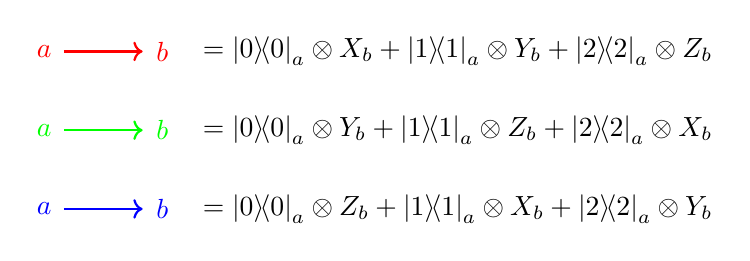
\begin{tikzpicture}
        \draw[->, red, thick] (0, 0) to (1, 0);
        \node[red] at (-0.25, 0) {$a$};
        \node[red] at (1.25, 0) {$b$};
        \node at (5, 0) {$= \dyad{0}_a \otimes X_b + \dyad{1}_a \otimes Y_b + \dyad{2}_a \otimes Z_b$};

        
        \draw[->, green, thick] (0, -1) to (1, -1);
        \node[green] at (-0.25, -1) {$a$};
        \node[green] at (1.25, -1) {$b$};
        \node at (5, -1) {$= \dyad{0}_a \otimes Y_b + \dyad{1}_a \otimes Z_b + \dyad{2}_a \otimes X_b$};


        \draw[->, blue, thick] (0, -2) to (1, -2);
        \node[blue] at (-0.25, -2) {$a$};
        \node[blue] at (1.25, -2) {$b$};
        \node at (5, -2) {$= \dyad{0}_a \otimes Z_b + \dyad{1}_a \otimes X_b + \dyad{2}_a \otimes Y_b$};
    \end{tikzpicture}
    }
    \label{eq:facet-commutators}
\end{equation}
Note that the gauged stabilizers are $\emph{not}$ unitary--- the qudit gauging procedure does not generically return unitary stabilizers. 

The self-dual version of the BB code introduced in examples above possesses the same transversal facet gate, although the logical action is more complicated, given the larger number of logical qubits. The physical implementation is the same however, and so the gauging procedure is very similar, up to modifying the connectivity of the gauging graph. The resultant stabilizers are pictured in Fig.~\ref{fig:facet-BB-stabilizers}. Again, since this self-dual BB code should be describable as a $\mathbb{Z}_2^{16}$ topological order, we conjecture this gauged model has $\mathbb{Z}_2^{16} \rtimes \mathbb{Z}_3$ topological order.

\begin{figure}[htbp]
    \centering
    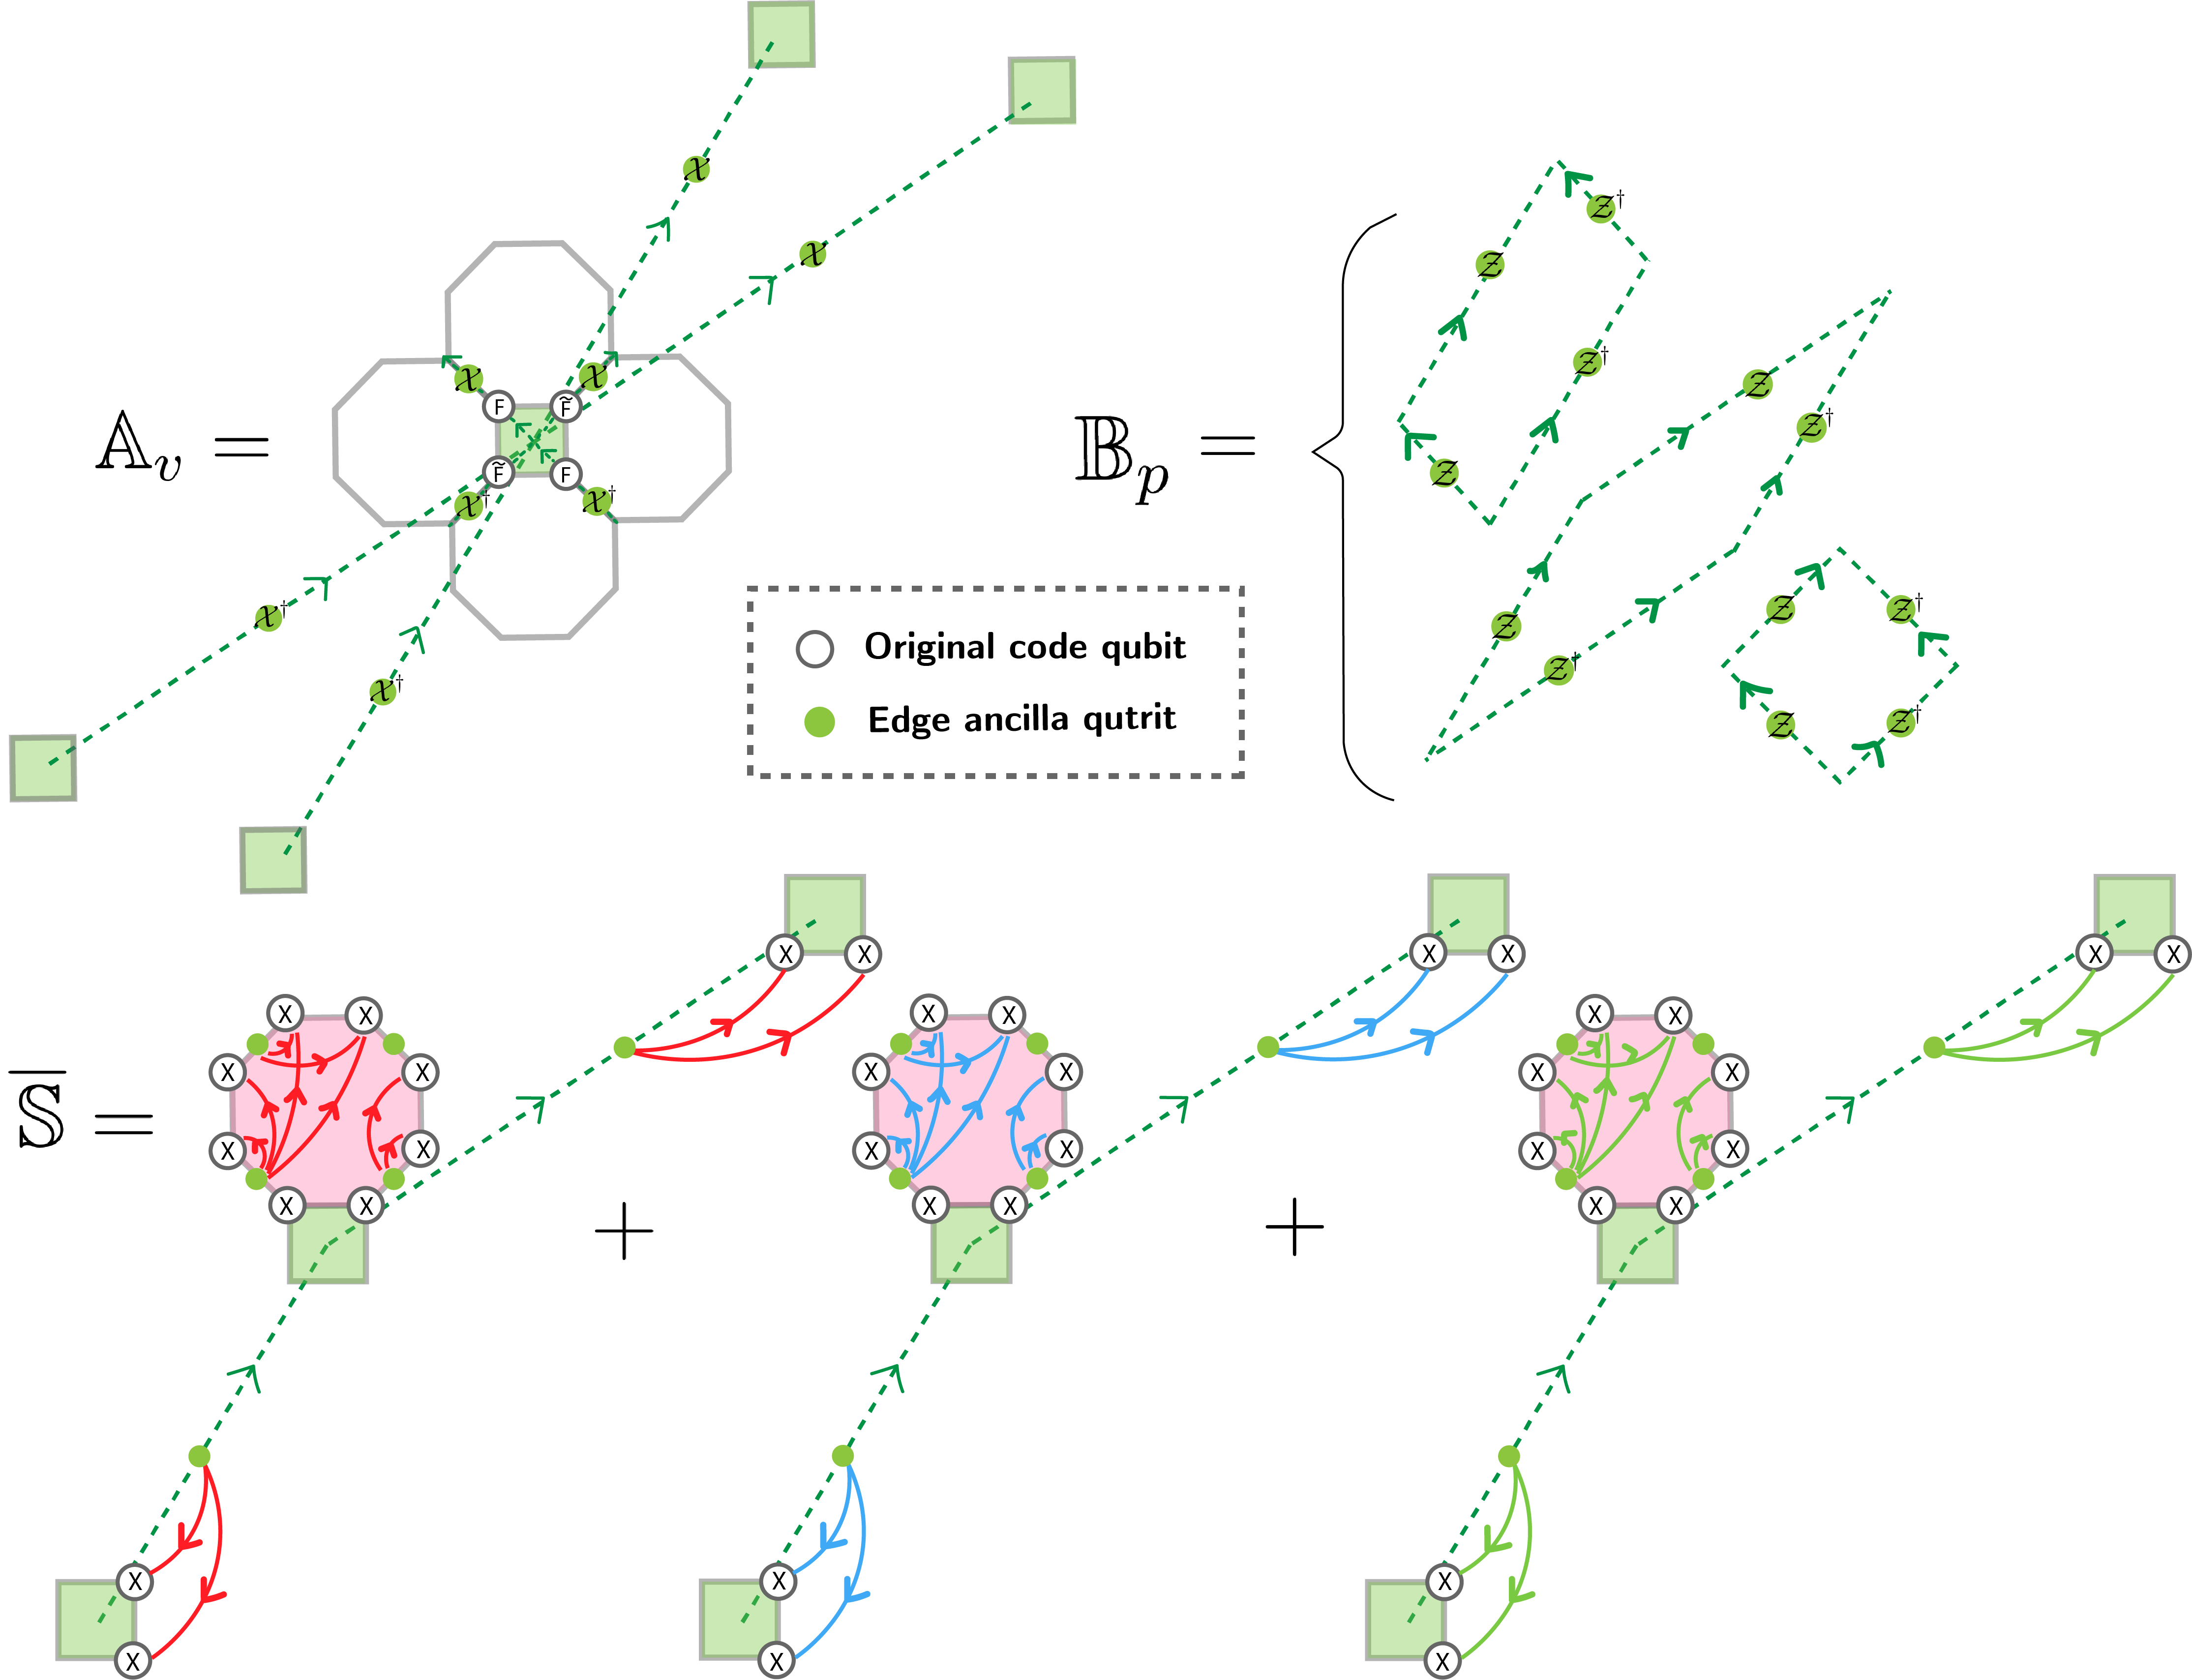
\includegraphics[width=1\linewidth]{figs/examples/hs-gauging-bb.png}
    \caption{\textbf{Gauging $HS$ on a Self-Dual BB Code:} We illustrate some of the stabilizers that result from gauging $HS$ on top of the self-dual BB code introduced at the beginning of the example section. The gauging graph is indicated by green dashed lines, while the grey lines denote the original lattice. The control gates used in $\gaugedS$ are defined in Eq.~\ref{eq:facet-commutators}.}
    \label{fig:facet-BB-stabilizers}
\end{figure}

\subsubsection{Charge conjugation on a qutrit BB code}
\begin{figure}[htbp]
    \centering
    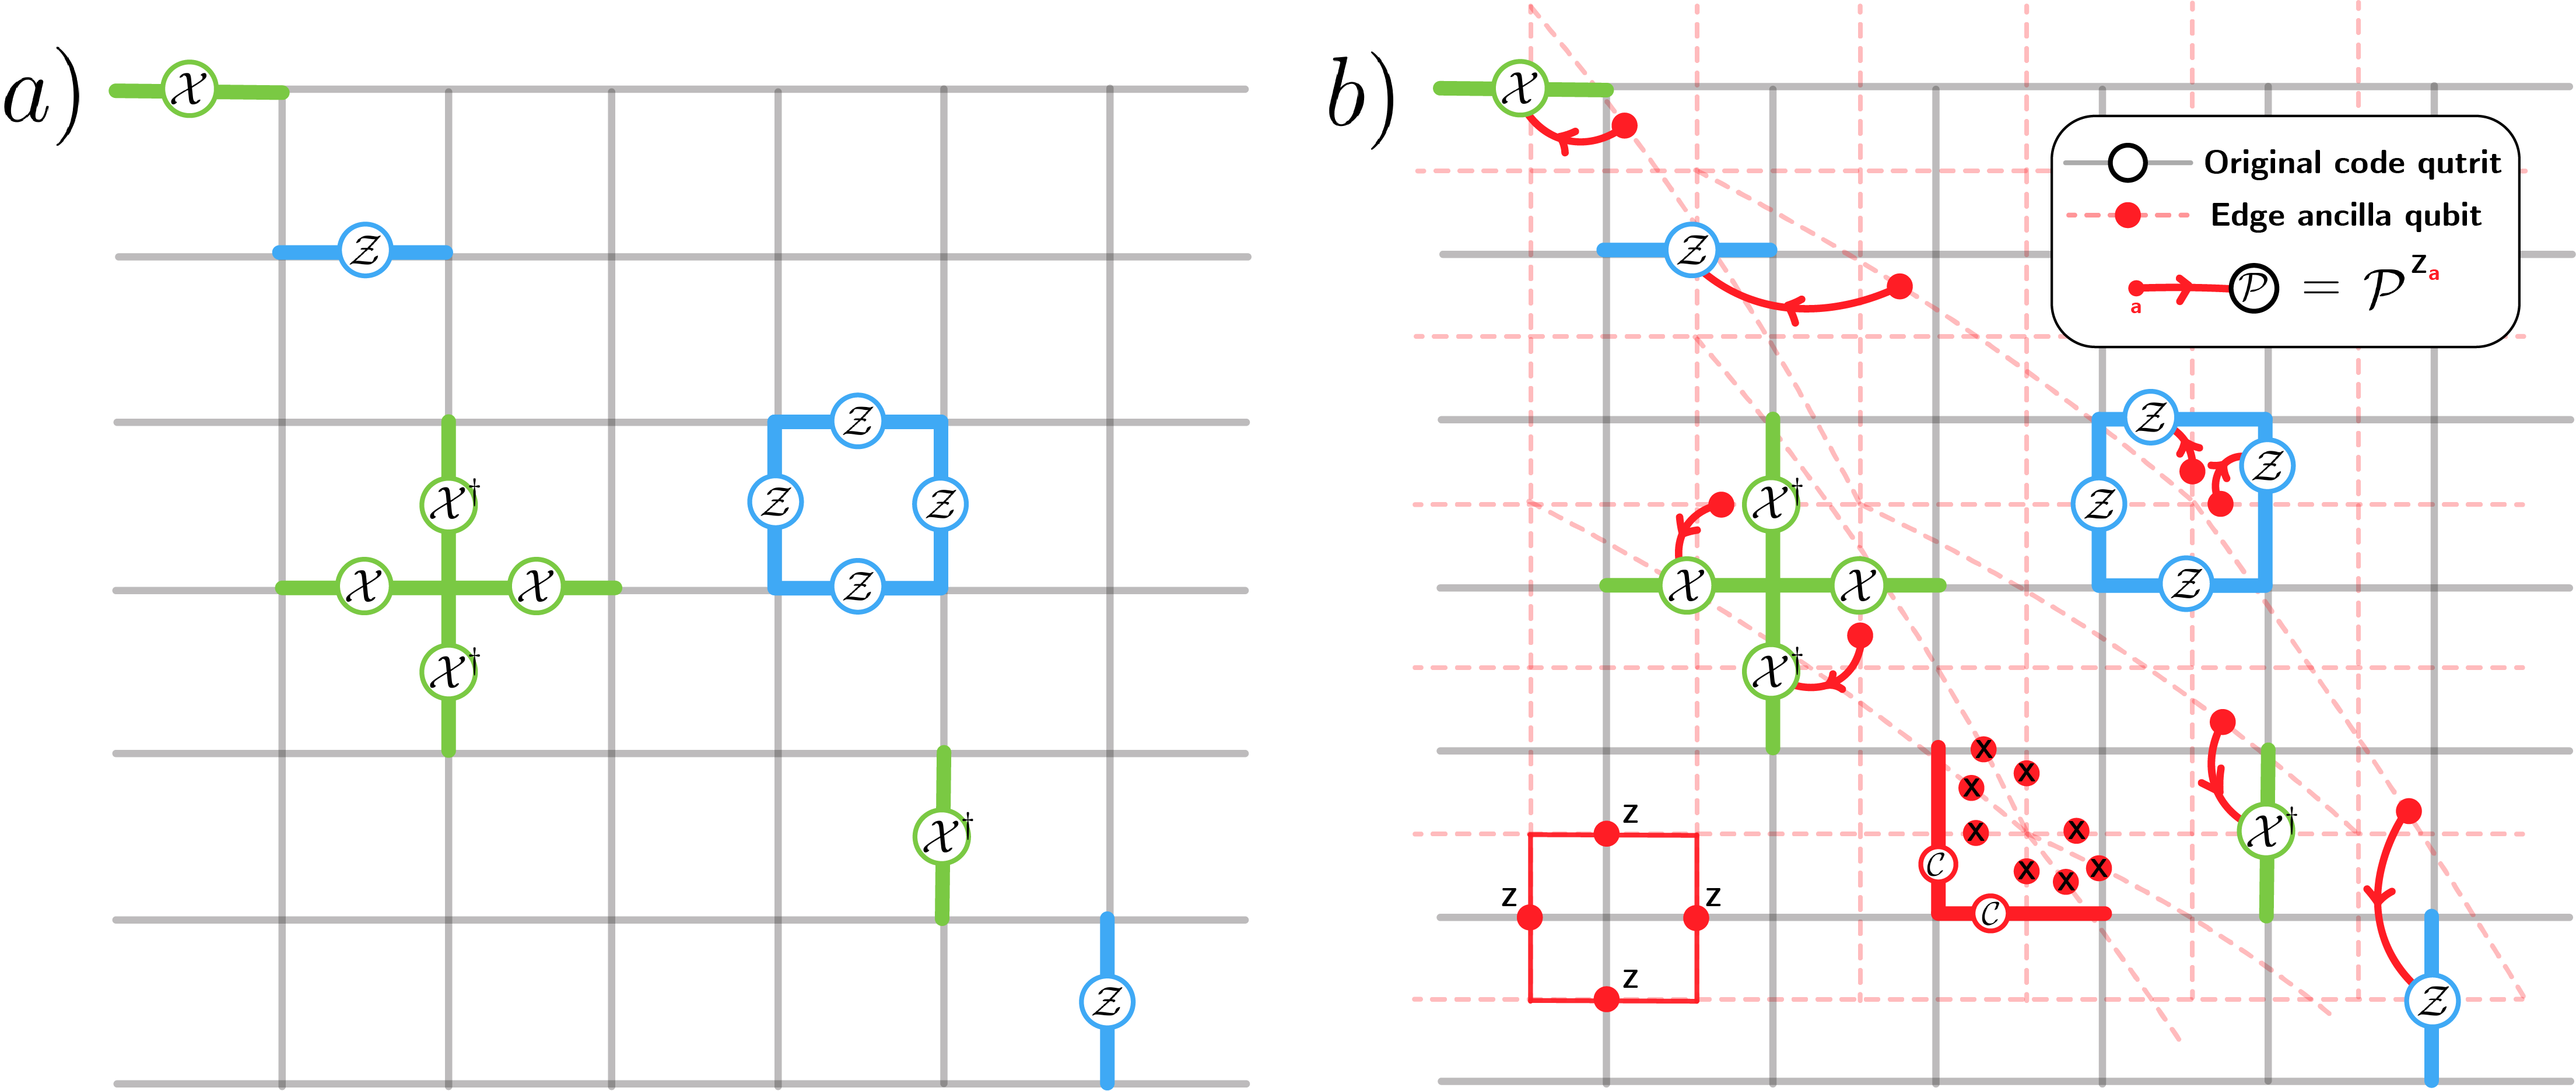
\includegraphics[width=1\linewidth]{figs/examples/S3-bb-example.png}
    \caption{\textbf{Gauging charge conjugation on the qutrit BB code:} a) Stabilizers for the initial qutrit code. b) Stabilizers for the code after gauging the $\mathbb{Z}_2$ symmetry. The gate $\mathcal{P}_i^{Z_j} = \dyad{0}_j \otimes \mathcal{P}_i + \dyad{1}_j \otimes \mathcal{P}^\dagger_i$ is a control gate with a \emph{qubit} control and a \emph{qutrit} target. Here, $\mathcal{P}$ is a tensor product of clock and shift operators. We have pictured unitary components of the decorated $\mathcal{X}$ and $\mathcal{Z}$ stabilizers (green and blue, respectively)--- note that the true stabilizers will be the sum of this component with its Hermitian conjugate. We also depict the vertex stabilizer $\av$ (bottom center) and an example cycle check $\bp$ (bottom left). }
    \label{fig:S3-BB-stabilizers}
\end{figure}

As an example starting with a non-qubit stabilizer code, consider the qutrit version of the $[[144, 12, 12]]$ Gross code. The Pauli operators are replaced with clock and shift operators: 
\begin{equation}
    \mathcal{ZX} = e^{2\pi i /3}\mathcal{XZ}, \mathcal{X}^3 = \mathcal{Z}^3 = \id
\end{equation}

The stabilizers are pictured in Fig.~\ref{fig:S3-BB-stabilizers}a. This model possesses a transversal charge conjugation gate, $\T = \prod \mathcal{C}$, where $\mathcal{C}$ acts as $\mathcal{C} \mathcal{X}^a \mathcal{Z}^b \mathcal{C} = \mathcal{X}^{-a} \mathcal{Z}^{-b}$. This is a $\mathbb{Z}_2$ symmetry. Choosing unit cells of the square lattice as our vertex set, the resultant stabilizers are pictured in Fig.~\ref{fig:S3-BB-stabilizers}b. 

Note that the logical action of $\T = \prod \mathcal{C}$ is to conjugate \emph{all} logical qutrits.

\subsubsection{Gauging qudit \texorpdfstring{$\CNOT$}{CNOT} on qudit CSS codes}
While the qudit gauging procedure generally returns non-unitary stabilizers, there are some special cases where we can find unitary stabilizers akin to the $\mathbb{Z}_2$ case. The structure of the resulting code is \emph{nilpotent}: in terms of the syndromes non-Abelian stabilizer violations always fuse to Abelian stabilizer violations. In terms of the stabilizers, we may always split the stabilizer group into two parts, one corresponding to (Abelian) stabilizers that only commute on the codespace, and the other to (non-Abelian) stabilizers that control those commutation relations. Essentially, the structure will always have the form of Corollary \ref{cor:z2-commutation-relations} in Sec. \ref{sec:gauging-procedure}.

Groups built from $\mathbb{Z}_2$ extensions of $\mathbb{Z}_2$ are always nilpotent, and so the qubit code/qubit symmetry case yields unitary stabilizers. Another class of nilpotent groups is $\mathbb{Z}_p^2 \rtimes \mathbb Z_p$; such a group would correspond to gauging a $\mathbb{Z}_q$ symmetry on two copies of a $q$-dimensional qudit code. A natural example of such a $\mathbb{Z}_p$ operator is qudit $\CNOT$ on two CSS qudit codes: 
\begin{equation}
    \CNOT_{a \to b} \ket{a} \ket{b} = \ket{a} \ket{b + a \text{ mod } q}
\end{equation}
The procedure to gauge this $\CNOT$ is the same as the qubit case, and results in much the same stabilizers, up to some daggers. See Fig.~\ref{fig:bb-qudit-CNOT} for the result of gauging qutrit $\CNOT$ on the qutrit BB code, using a single edge of the square lattice as a vertex set. It is instructive to compare this example to the earlier qubit BB code.

\begin{figure}[htbp]
    \centering
    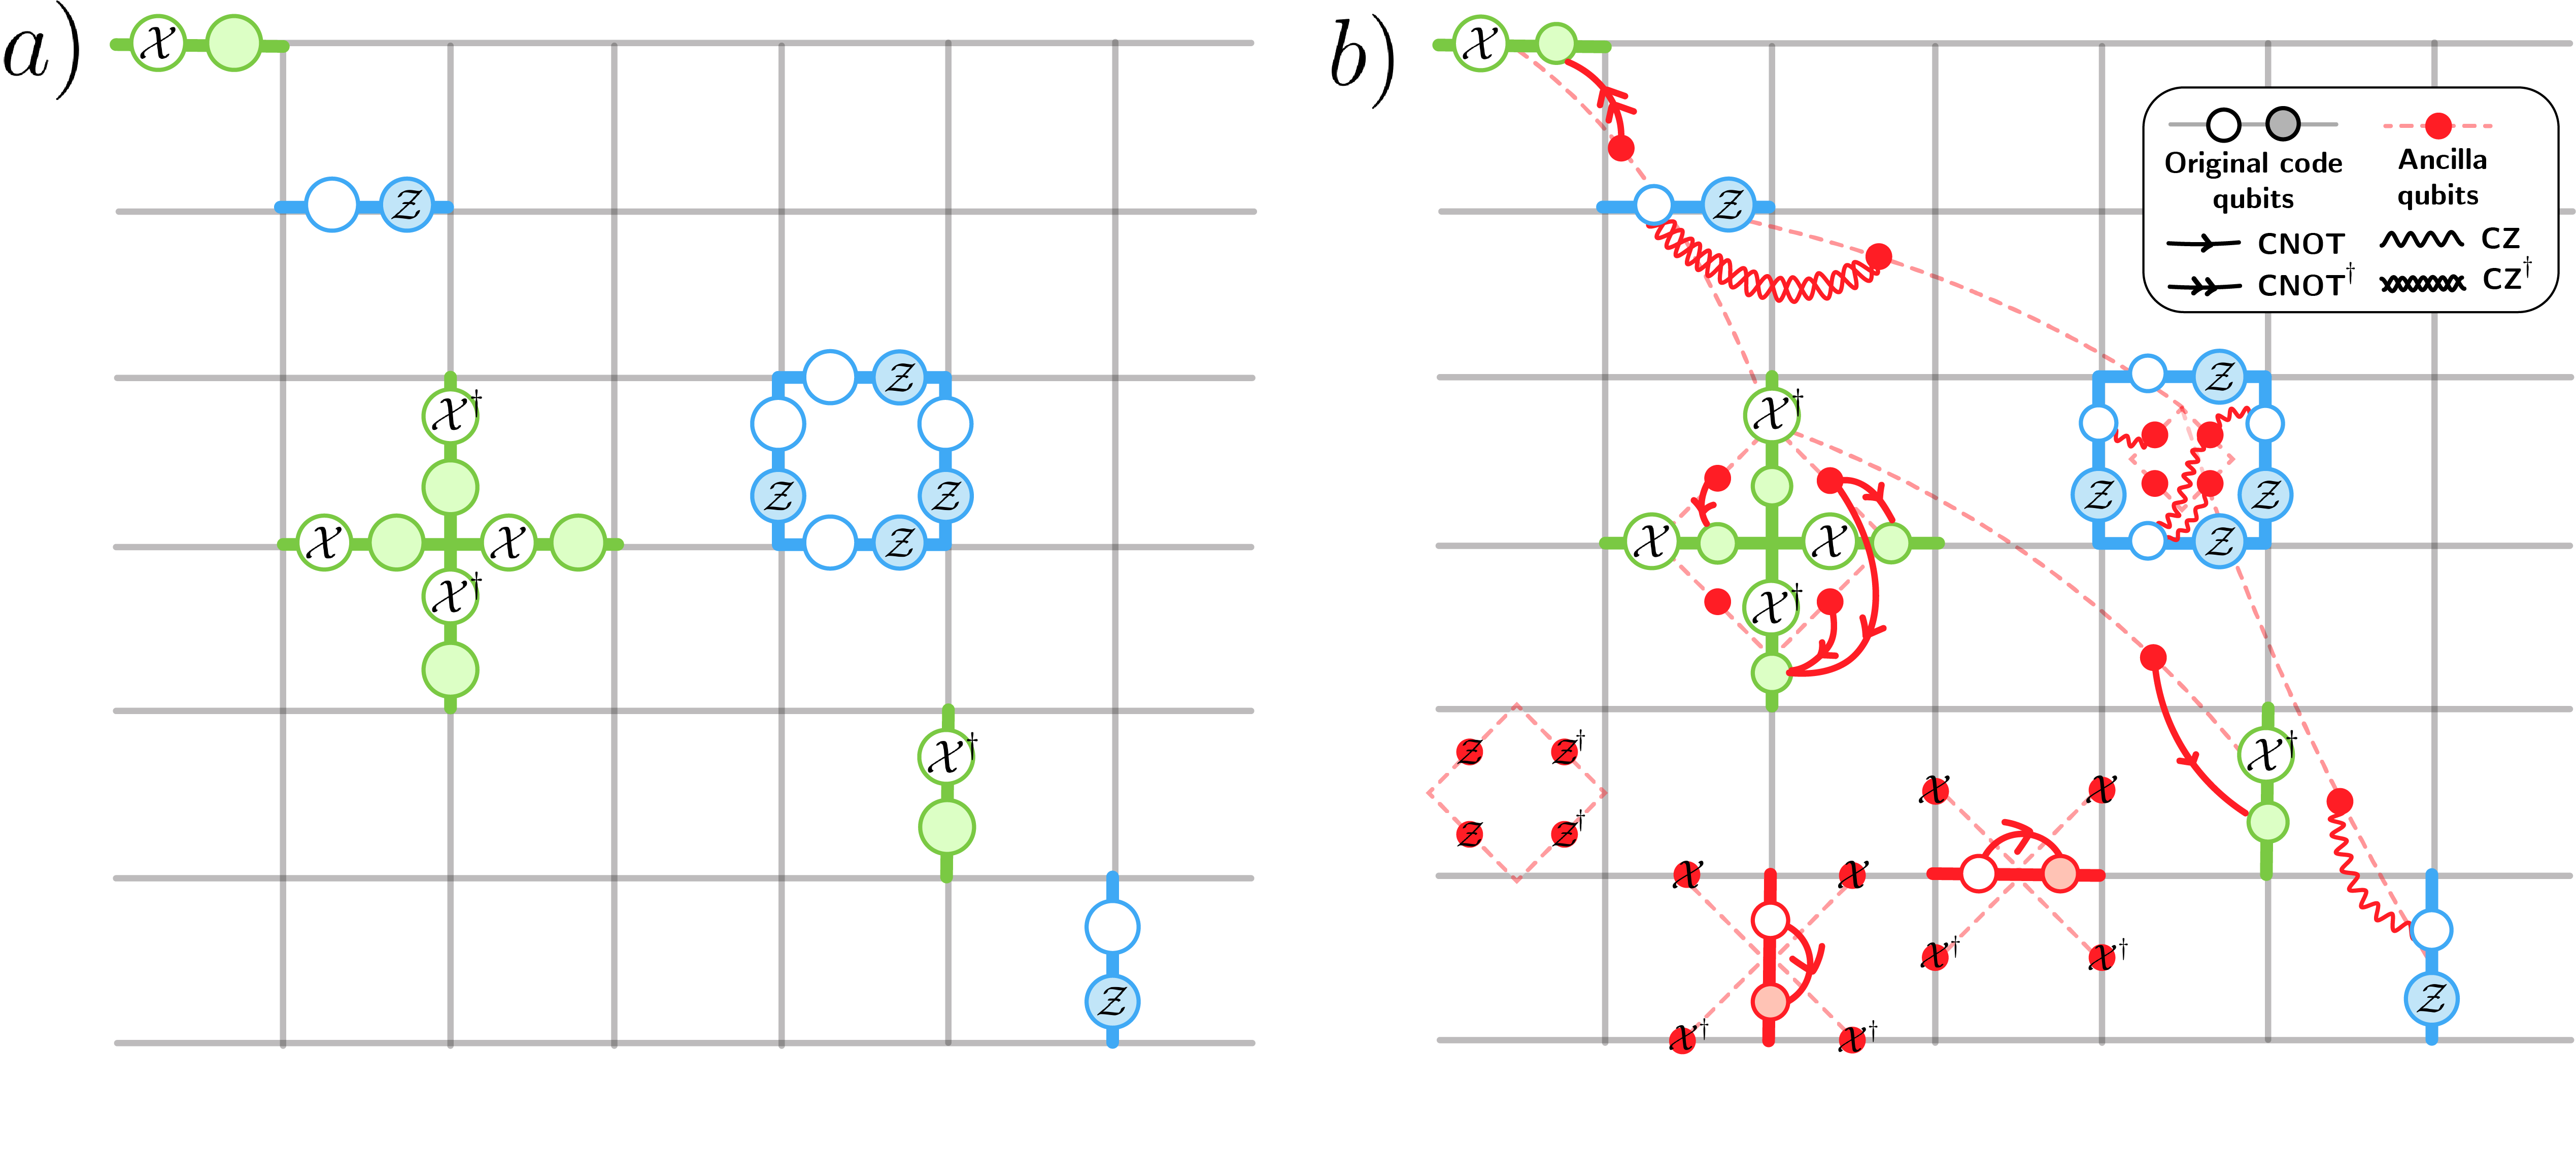
\includegraphics[width=1\linewidth]{figs/examples/bb-qutrit-cnot.png}
    \caption{\textbf{Gauging $\CNOT$ on the qutrit BB code:} a) Stabilizers for the initial qutrit code. We have only pictured the stabilizers that are affected by the gauging procedure. b) Stabilizers for the code after gauging transversal qutrit $\CNOT$. We have taken the pair of qutrits belonging to the same edge in the two codeblocks as a vertex set. We have omitted depicting the full gauging graph for visual clarity, but it has the same connectivity as in Fig.~\ref{fig:bb_cnot_gauging}.}
    \label{fig:bb-qudit-CNOT}
\end{figure}


\subsection{Fold-transversal gates on hypergraph product codes}

In this example we gauge a fold-transversal $\mathbb{Z}_2$ symmetry on a generic square hypergraph product (HGP) code \cite{Breuckmann2024, Quintavalle_2023}. We define a choice of vertex sets compatible with the structure of the fold transversal gates defined in Ref.~\cite{Breuckmann2024}, and derive the resulting gauged code.

Recall the hypergraph product of two classical codes $\mathcal{C}_1: C_1^{(1)}\overset{H_1}{\rightarrow} C_0^{(1)}$ and $\mathcal{C}_2:C_1^{(2)}\overset{H_2}{\rightarrow}C_0^{(2)}$ is the quantum code associated to the tensor product chain complex: 
\begin{equation}
    \mathcal{C} = \mathcal{C}_1 \otimes \mathcal{C}_2: C_1^{(1)} \otimes C_1^{(2)} \overset{H_X}{\rightarrow} C_0^{(1)} \otimes C_1^{(2)} \oplus C_1^{(1)} \otimes C_0^{(2)} \overset{H^T_Z}{\rightarrow} C_0^{(1)} \otimes C_0^{(2)}
\end{equation}
\begin{align}
    H_X = (H_1\otimes I_{n_2}\ |\ I_{n_1}\otimes H_2)\\
    H_Z = (I_{m_1}\otimes H^T_2\ |\ H_1^T\otimes I_{m_2})
\end{align}
If $\mathcal{C}_2 = \mathcal{C}_1^T$ is the dual classical code of $\mathcal{C}_1$, then the quantum code $\mathcal{C}$ is a \emph{square} HGP code. If the input classical code is self-dual, then $\mathcal{C}$ is a \emph{symmetric} HGP code.

Square codes may possess transversal Clifford gates of the following form \cite{Breuckmann2024}: 
\begin{equation}
    \T_\tau = \bigotimes_{\substack{i = 1, \dots, n \\ i < \tau(i)}} \text{SWAP}_{i, \tau(i)} \bigotimes_{i = 1}^n H_i
\end{equation}
where $\tau$ is a permutation on the labels of physical qubits. We assume $\tau^2 = \id$, which allows us to break the circuit of $\text{SWAP}$ gates into disjoint local actions, and ensures that $\T^2 = \id$. For a general permutation $\tau$, we must include the entire orbit of a given qubit in a vertex set, and the order of the gate $\T$ becomes larger than 2, necessitating gauge qudits.

We define vertex sets $\invvertexset{v_i} = \{i, \tau(i)\}$ for $i \leq \tau(i)$. The associated local action of $\T_\tau$ is 
\begin{equation}
    (\T_\tau)_{v_i} \equiv (\T_\tau)_i = \text{SWAP}_{i, \tau(i)} H_i H_{\tau(i)}, \quad \T_\tau = \bigotimes_{i < \tau(i)} (\T_\tau)_i.
\end{equation}
As $\tau^2 = \id$, we have at most order-2 orbits for each qubit, and also at most order-2 orbits for the stabilizers. In particular, each $Z$ stabilizer $S_Z$ is paired with an $X$ stabilizer $S_X = \tau(S_Z)$ to form the orbit $O(S_Z) = \{S_Z, \tau(S_Z)\}$. Thus, the commutation relation between any stabilizer and the local symmetry action is:
\begin{equation}
\ComGrp{S_Z}{(\T_\tau)_i} = \left [(\tau(S_Z))_i \prod_{j \neq i}(S_Z)_j \right ] S_Z = [\tau(S_Z)]_i (S_Z)_i 
\end{equation}
We require a short path connecting any two vertex ancillas whose vertex sets have support on the same stabilizer. Assuming we have constructed the gauging graph with such short paths, the gauged stabilizers are:\footnote{Due to the LDPCness of the initial HGP code, we can always construct this gauging graph while preserving bounded degree by simply adding an edge whenever a short path is missing.}
\begin{equation}
    \av = (\T_\tau)_i \prod_{e \in \delta v_i} X_e, \quad \bp = \prod_{\substack{e \in f \\ \partial f = 0}} Z_e,
\end{equation}
\begin{equation}
    \gaugedS = S \cdot \left ( \prod_{i \neq i_0} \prod_{e \in p(i, i_0)} C_e (\tau(S))_i C_e S_i \right ).
\end{equation}
See Fig.~\ref{fig:fold-transversal-gauging} for an illustration of these stabilizers in the simplest case of the fold transversal gate on the surface code \cite{Moussa_2016}.
We emphasize that this procedure applies to any square HGP code, but we choose to illustrate the surface code for the sake of clarity in the presentation of the figure.

\begin{figure}
    \centering 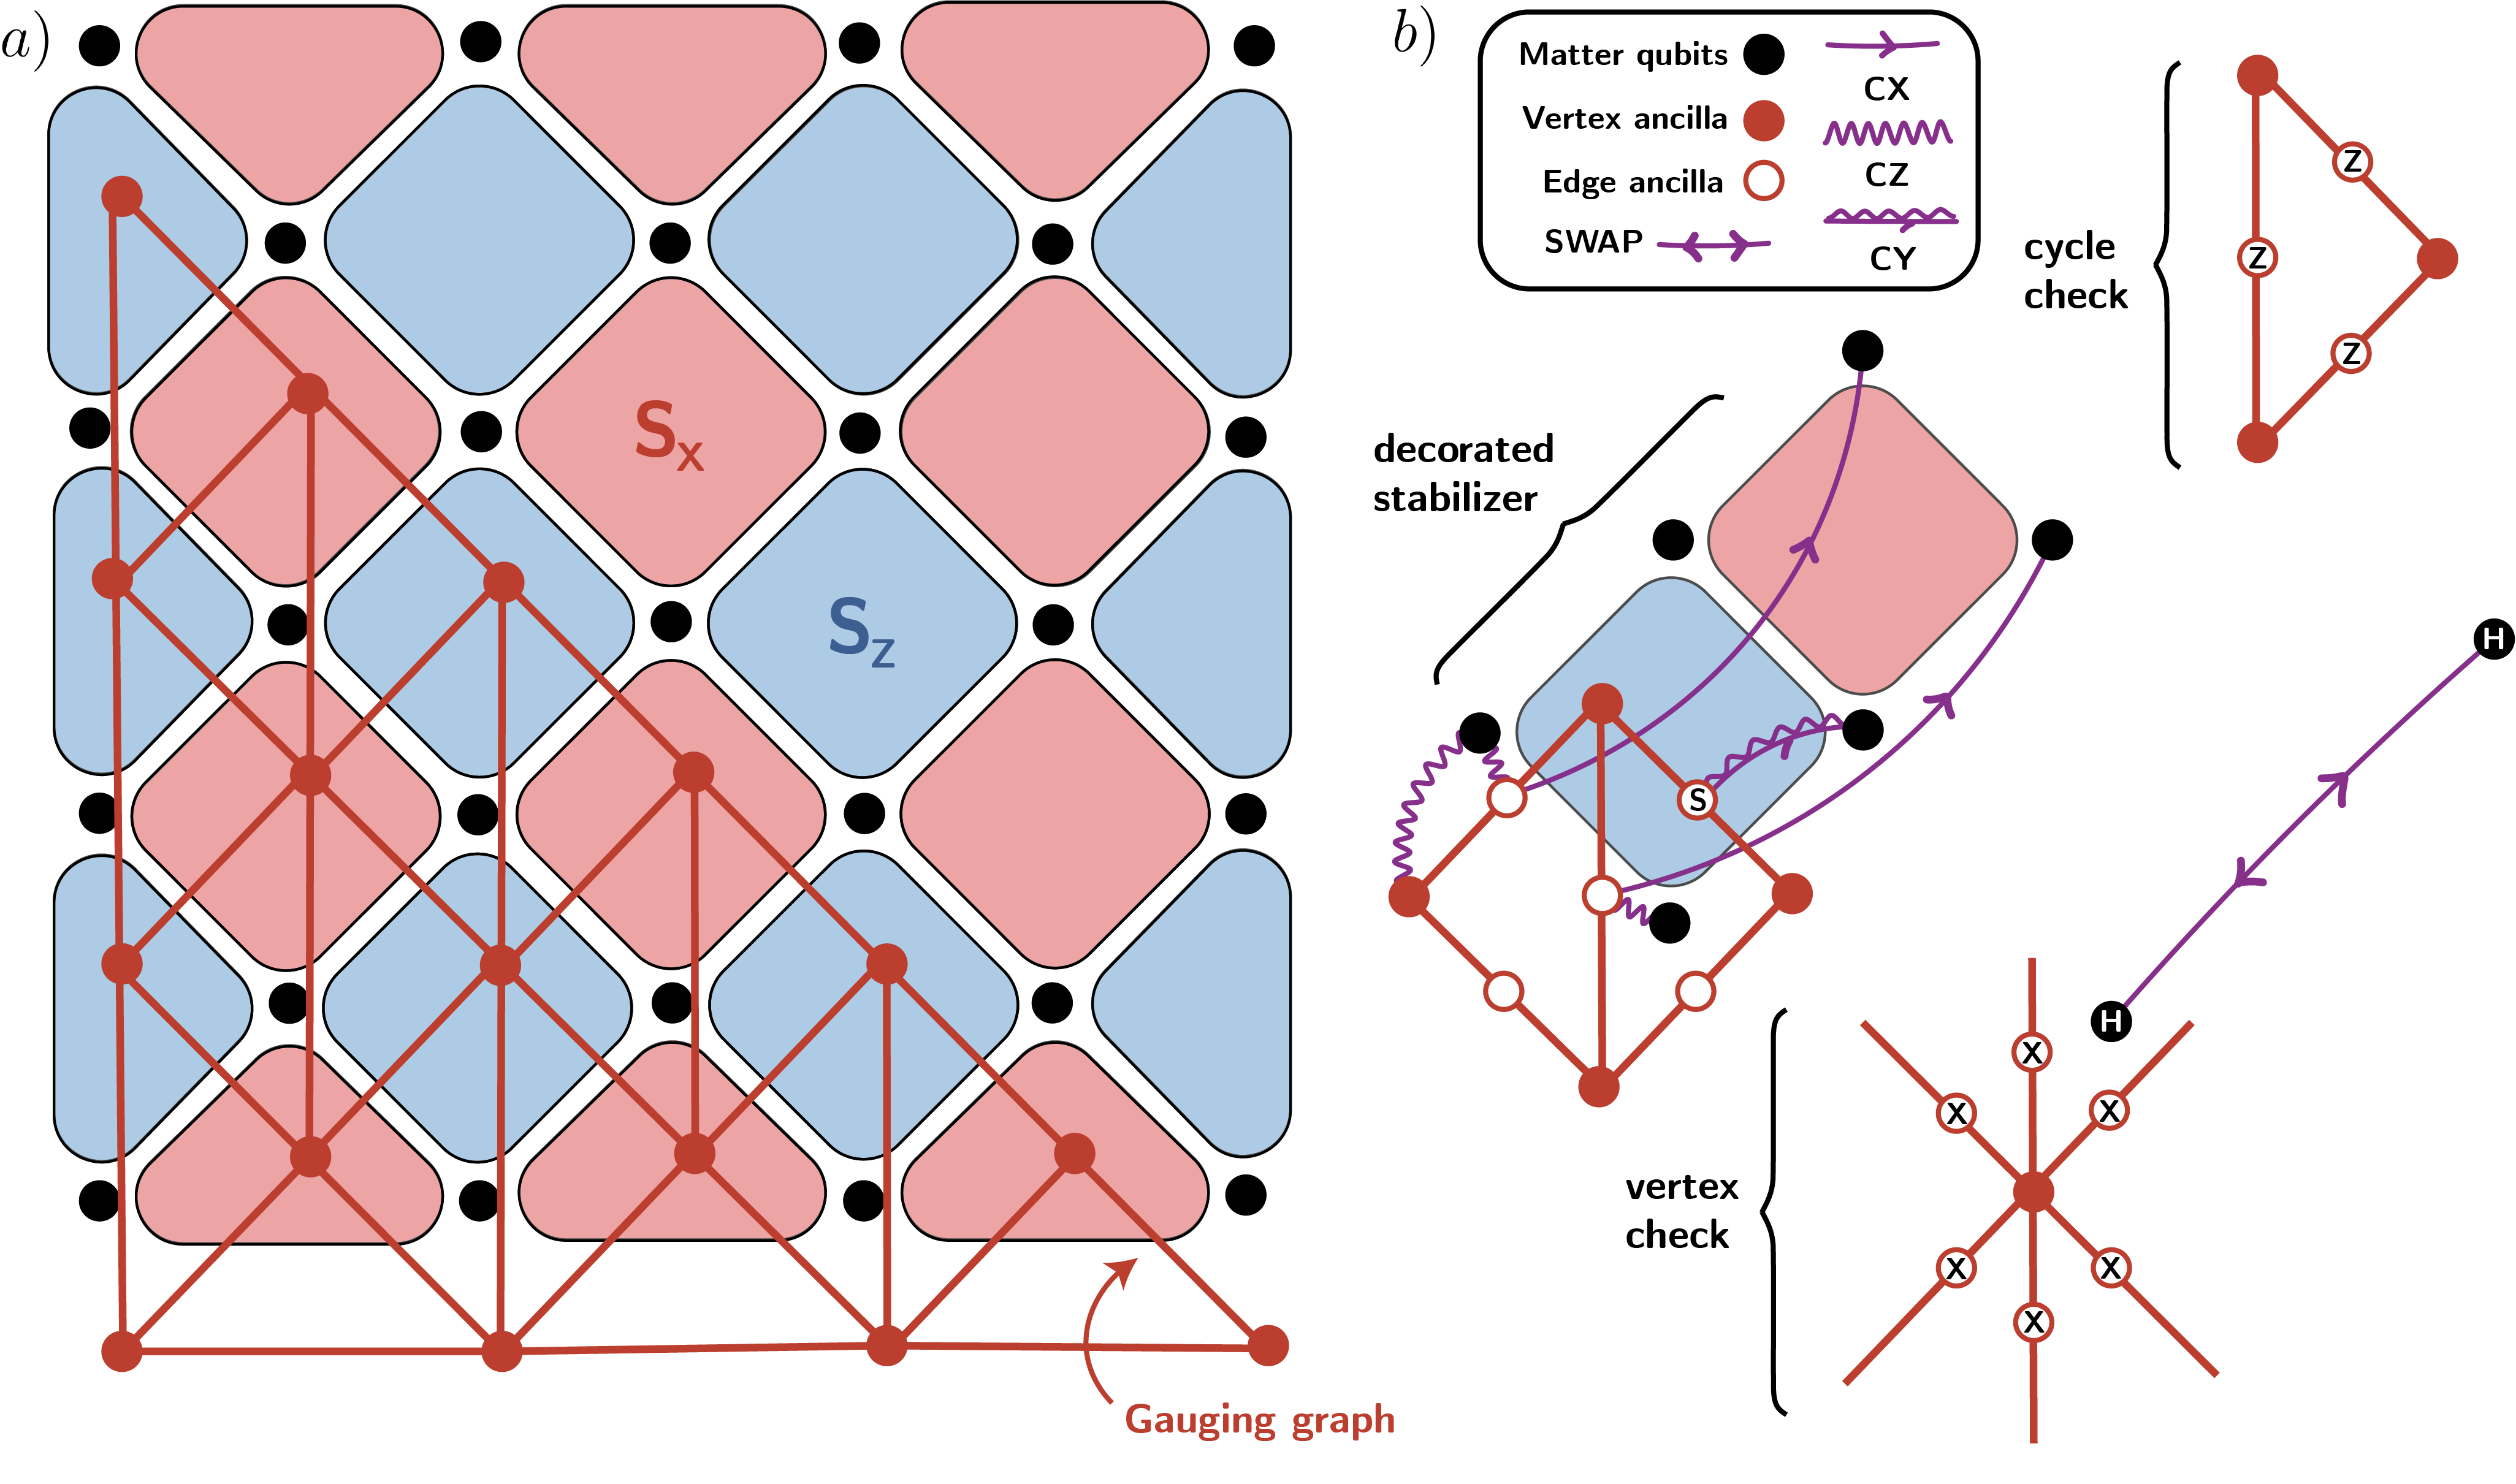
\includegraphics[width=0.75\linewidth]{figs/fold-transversal-gauging.png}
    \caption{a) Consider the fold transversal Hadamard gate on the surface code, which exchanges $S_X$ (pink) and $S_Z$ (blue) stabilizers along the diagonal running from the top left to the bottom right.  A convenient choice of gauging graph is given in the figure (red lines). b) The resulting gauged stabilizers. }
    \label{fig:fold-transversal-gauging}
\end{figure}


\ifdefined\ismainfile
\else
    \bibliography{bib}
    \end{document}
\fi
